\documentclass{article}
\usepackage{amsmath}

\usepackage[final]{neurips}
\usepackage{subcaption}
\usepackage{enumitem}
% to avoid loading the natbib package, add option nonatbib:
% \usepackage[nonatbib]{neurips_2019}
\usepackage{setspace} % Include the setspace package in your preamble
\usepackage{listings}
\usepackage[dvipsnames]{xcolor}
% To set one-and-a-half spacing:
\onehalfspacing
\usepackage[utf8]{inputenc} % allow utf-8 input
% \usepackage{natbib}
% \let\citep\cite
% \let\citelatin\cite
% \let\citeplatin\cite
\usepackage{titlesec}
\titleformat{\section}
{\normalfont\LARGE\bfseries}{\thesection}{1em}{}
\titleformat{\subsection}
{\normalfont\large\bfseries}{\thesubsection}{1em}{}
\usepackage[T1]{fontenc}    % use 8-bit T1 fonts
\usepackage{xcolor} % مطمئن شوید این پکیج قبل از hyperref فراخوانی شده باشد
\usepackage{hyperref}


\hypersetup{
	colorlinks=true,
	linkcolor=MidnightBlue,  % رنگ پیوندهای داخلی و فهرست
	filecolor=magenta,        
	urlcolor=blue!80!black,   
	citecolor=teal
}

% اضافه کردن آپشن titles برای حل تداخل با بسته‌های دیگر
\usepackage[titles, subfigure]{tocloft}

% ۱. وسط‌چین کردن و تغییر رنگ عنوان «فهرست مطالب» به 


% ۲. تغییر رنگ شماره صفحه‌ها در فهرست مطالب به MidnightBlue
\renewcommand{\cftsecpagefont}{\color{MidnightBlue}}
\renewcommand{\cftsubsecpagefont}{\color{MidnightBlue}}
\renewcommand{\cftsubsubsecpagefont}{\color{MidnightBlue}}

% ۳. کد اصلاح‌شده برای تغییر رنگ خط‌چین‌ها به MidnightBlue بدون ارور
\renewcommand{\cftsecleader}{\color{MidnightBlue}\cftdotfill{\cftdotsep}}
\renewcommand{\cftsubsecleader}{\color{MidnightBlue}\cftdotfill{\cftdotsep}}


% \usepackage{xcolor}
\usepackage{tcolorbox}
\setcounter{footnote}{0} 
\usepackage{amsmath} 
\usepackage{url}            % simple URL typesetting
\usepackage{booktabs}       % professional-quality tables
\usepackage{amsfonts}       % blackboard math symbols
\usepackage{nicefrac}       % compact symbols for 1/2, etc.
\usepackage{microtype}      % microtypography
\usepackage{graphicx}
\usepackage{float}

% بسته‌های اضافه شده برای رسم نمودار
\usepackage{tikz}
\usepackage{pgfplots}

\usepackage{xepersian}
\settextfont{XB Yas.ttf}



% The \author macro works with any number of authors. There are two commands
% used to separate the names and addresses of multiple authors: \And and \AND.
%
% Using \And between authors leaves it to LaTeX to determine where to break the
% lines. Using \AND forces a line break at that point. So, if LaTeX puts 3 of 4
% authors names on the first line, and the last on the second line, try using
% \AND instead of \And before the third author name.


\renewcommand{\lstlistingname}{Code}

\definecolor{codegreen}{rgb}{0,0.6,0}
\definecolor{codegray}{rgb}{0.5,0.5,0.5}
\definecolor{codepurple}{rgb}{0.58,0,0.82}
\definecolor{backcolour}{HTML}{FDF6E3}

\lstdefinestyle{mystyle}{
	backgroundcolor=\color{backcolour},   
	commentstyle=\color{codegreen},
	keywordstyle=\color{magenta},
	numberstyle=\tiny\color{codegray},
	stringstyle=\color{codepurple},
	basicstyle=\ttfamily\footnotesize,
	breakatwhitespace=false,         
	breaklines=true,                 
	captionpos=b,                    
	keepspaces=true,                 
	numbers=left,                    
	numbersep=5pt,                  
	showspaces=false,                
	showstringspaces=false,
	showtabs=false,                  
	tabsize=2
}

\usepackage{listings}
\usepackage{xcolor}

\lstset{
	basicstyle=\small\ttfamily,
	numbers=left,
	numberstyle=\tiny\color{gray},
	stepnumber=1,
	numbersep=8pt,
	showstringspaces=false,
	tabsize=4,
	breaklines=true,
	breakatwhitespace=false,
	keepspaces=true,           % جهت حفظ دقیق فاصله‌های ابتدای خط (Indent)
	frame=single
}

\pgfplotsset{compat=1.16}
\lstset{style=mystyle}

\begin{document}
	
\begin{titlepage}
	\centering
	
	
\includegraphics[width=0.4\textwidth]{img/logos/Logo.png} \\[1cm]
	
	% نام دانشگاه
	{\Huge\textbf{دانشگاه صنعتی خواجه نصیرالدین طوسی}}\\[0.3cm]
	{\Large دانشکده مهندسی برق}\\[2cm]
	
	% عنوان پروژه
	{\fontsize{18pt}{28pt}\selectfont
		\textbf{بازرسی بصری خودکار}\\[0.3cm]
		{\Large از تشخیص شیء تا قطعه‌بندی ناهنجاری}
	}\\[2cm]
	
	% مشخصات تهیه‌کنندگان
	% تیم مجری پروژه
	{\Large\textbf{پروژه توسط}}\\[0.25cm]
	{\fontsize{22pt}{28pt}\selectfont
		\bfseries
		\textcolor{MidnightBlue}{تیم شیر}
	}\\[0.8cm]
	
	{\fontsize{14pt}{22pt}\selectfont
		\textbf{اعضای تیم}\\[0.4cm]
		مصطفی لطیفیان - ۴۰۱۲۲۱۹۳\\
		پارسا علوی نیکو - ۴۰۱۲۰۹۹۳\\[0.25cm]
		حمیدرضا عابدینی - ۴۰۱۲۰۶۳۳
	}\\
	
	% لوگوهای لینک‌دار
	\begin{center}
		\href{https://colab.research.google.com/drive/1xZcyCR2VT2tJiZzI3_5DCzFtpvebPqOK}{
\includegraphics[height=1cm]{img/logos/colab_logo.png}}
		\hspace{0.8cm}
		\href{https://drive.google.com/drive/u/0/folders/1WZ09zYK7gx8-aRyjB2l2r8C4PhFr2-d5}{
\includegraphics[height=1cm]{img/logos/drive_logo.png}}
		\hspace{0.8cm}
		\href{https://github.com/parsaalv/Automated-Visual-Inspection}{
\includegraphics[height=1cm]{img/logos/github_logo.png}}
	\end{center}
	
\end{titlepage}

\newpage


\tableofcontents
\newpage % برای اینکه متن اصلی از صفحه بعد شروع شود
% عنوان اصلی بدون شماره اما حاضر در فهرست مطالب
\section*{مقدمه و معرفی جامع دیتاست}
\addcontentsline{toc}{section}{مقدمه و معرفی جامع دیتاست}

\subsection*{معرفی دیتاست MVTec AD}
\addcontentsline{toc}{subsection}{معرفی دیتاست MVTec AD}
در سیستم‌های بینایی ماشین صنعتی (\lr{Industrial Machine Vision})، یکی از بزرگترین چالش‌ها، کمبود داده‌های مربوط به قطعات معیوب است. در خطوط تولید واقعی، اکثر قطعات سالم هستند و تولید یک مجموعه داده متوازن از انواع خرابی‌ها تقریباً غیرممکن است. به همین دلیل، در این پروژه از مجموعه داده استاندارد و معتبر \lr{MVTec Anomaly Detection (MVTec AD)} استفاده شده است.

این دیتاست به‌عنوان استاندارد طلایی (\lr{Gold Standard}) برای ارزیابی الگوریتم‌های تشخیص ناهنجاریِ نظارت‌نشده (\lr{Unsupervised Anomaly Detection}) شناخته می‌شود. رویکرد نظارت‌نشده به این معناست که سیستم هوش مصنوعی در فاز آموزش، تنها و تنها تصاویر قطعات کاملاً سالم را مشاهده می‌کند تا «مفهوم نرمال بودن» را یاد بگیرد؛ سپس در فاز تست، هرگونه انحراف از این حالتِ نرمال را به‌عنوان ناهنجاری (\lr{Defect}) شناسایی می‌کند.

\subsection*{ساختار و معماری داده‌ها}
\addcontentsline{toc}{subsection}{ساختار و معماری داده‌ها}
تصاویر موجود در این مجموعه داده با وضوح بالا (\lr{High-Resolution}) ثبت شده‌اند و به گونه‌ای طراحی شده‌اند که شرایط واقعی یک کارخانه (مانند تغییرات نور، زاویه قرارگیری و بازتاب‌های نوری) را شبیه‌سازی کنند. ساختار پوشه‌بندی دیتاست برای هر قطعه به شرح زیر است:

\begin{itemize}
	\item \textbf{مجموعه آموزش (\lr{Train Set}):} شامل تصاویری از قطعات ۱۰۰٪ سالم (\lr{Good}).
	\item \textbf{مجموعه آزمون (\lr{Test Set}):} شامل ترکیبی از تصاویر سالم و تصاویری با انواع خرابی‌های ساختاری و ظاهری (مانند شکستگی، خراش، خمیدگی، تغییر شکل و قطعات مفقود شده).
	\item \textbf{حقیقت مبنا (\lr{Ground Truth}):} برای تمام تصاویر معیوب در مجموعه آزمون، ماسک‌های دقیق در سطح پیکسل (\lr{Pixel-level Annotations}) ارائه شده است. این ماسک‌ها (که دقیقاً روی نواحی خراب قرار می‌گیرند) برای ارزیابی دقیق مدل در فاز مکان‌یابی عیوب (\lr{Localization \& Segmentation}) استفاده می‌شوند.
\end{itemize}

\subsection*{تنوع کلاس‌ها و چالش‌های پردازشی}
\addcontentsline{toc}{subsection}{تنوع کلاس‌ها و چالش‌های پردازشی}
در این پروژه، ۶ کلاسِ شیء (\lr{Object-type}) کاملاً متمایز انتخاب شده‌اند تا قدرت تعمیم‌پذیری (\lr{Generalization}) مدل معماری‌شده به چالش کشیده شود:

\begin{itemize}
	\item \textbf{بطری (\lr{Bottle}):} چالش بازتاب نور روی سطوح شفاف و شیشه‌ای.
	\item \textbf{کابل (\lr{Cable}):} چالش بافت‌های تکرارشونده و در هم تنیده با رنگ‌های مختلف.
	\item \textbf{مهره فلزی (\lr{Metal Nut}):} چالش سطوح براق فلزی و سایه‌های متغیر.
	\item \textbf{پیچ (\lr{Screw}):} چالش تشخیص خراش‌های بسیار ریز میکروسکوپی روی رزوه‌های فلزی.
	\item \textbf{مسواک (\lr{Toothbrush}):} چالش بافت بسیار متراکم و نویزدار در قسمت موهای مسواک.
	\item \textbf{ترانزیستور (\lr{Transistor}):} چالش بررسی هندسه دقیق و جایگذاری صحیح پین‌ها در مدارهای الکترونیکی.
\end{itemize}

\subsection*{رویکرد داده‌محور (\lr{Data-Centric AI}) و پیش‌پردازش سفارشی}
\addcontentsline{toc}{subsection}{رویکرد داده‌محور (\lr{Data-Centric AI}) و پیش‌پردازش سفارشی}
یکی از اصول اساسی در مهندسی هوش مصنوعیِ واقعی این است که مجموعه داده‌ها همیشه بی‌نقص نیستند. در طول بررسی اکتشافی داده‌ها (\lr{EDA}) در این پروژه، مشخص شد که حاشیه‌نویسی‌ها (\lr{Annotations}) و ماسک‌های مربوط به کلاس ترانزیستور (\lr{Transistor}) دارای تداخل و خطاهای ساختاری هستند (تشخیص یکپارچه تمامی ناهنجاری‌ها به جای تفکیک آن‌ها).

برای رفع این مشکل بنیادین، از رویکرد هوش مصنوعی داده‌محور (\lr{Data-Centric AI}) استفاده شد. به جای تغییر معماری مدل، داده‌های خام به پلتفرم تخصصی \lr{Roboflow} منتقل شدند. در این پلتفرم، باندینگ باکس‌ها (\lr{Bounding Boxes}) و ماسک‌های کلاس ترانزیستور مجدداً توسط انسان بررسی، اصلاح و کالیبره شدند. این مداخله مهندسی تضمین کرد که \lr{Ground Truth} ارائه‌شده به مدل برای محاسبه خطا (\lr{Loss}) و ارزیابی نهایی، دارای بالاترین سطح اعتبار و دقت (\lr{Fidelity}) باشد.


\section{گردآوری مجموعه داده، ساختاردهی و آماده‌سازی برای تکرارپذیری}

مرحله اول پروژه به آماده‌سازی زیرساخت داده‌ها، تضمین تکرارپذیری آزمایش‌ها و ایجاد پایپ‌لاین دریافت و پالایش خودکار دیتاست اختصاص دارد. این مرحله زیربنای تمامی فازهای بعدی آموزش و ارزیابی مدل است.

\subsection{اتصال به فضای ذخیره‌سازی ابری (\lr{Load from Google Drive})}

در محیط‌های پردازش ابری موقت (مانند \lr{Google Colab})، با هر بار قطع شدن نشست (\lr{Session})، تمامی داده‌ها و مدل‌های آموزش‌دیده از بین می‌روند. برای حفظ پیوستگی پروژه در فازهای مختلف تحقیق و توسعه، استفاده از یک فضای ذخیره‌سازی پایدار (\lr{Persistent Storage}) الزامی است تا نتایج هر مرحله به عنوان ورودی مرحله بعد، به‌صورت امن ذخیره شود.
با استفاده از کتابخانه \lr{\texttt{google.colab}} و ماژول \lr{\texttt{drive.mount}}، فضای \lr{Google Drive} کاربر به محیط لینوکسیِ کولب متصل (\lr{Mount}) می‌شود. سپس مسیر اصلی پروژه در متغیر \lr{\texttt{PROJECT\_DIR}} تعریف شده و با تابع \lr{\texttt{os.path.exists}} صحت این اتصال و وجود مسیر ذخیره‌سازی بررسی می‌گردد.

\subsection{دریافت و آماده‌سازی داده‌ها از کگل (\lr{Load from Kaggle})}

این بخش شامل زنجیره‌ای از ۷ فرآیند مهندسی داده برای ساخت پایپ‌لاین دریافت، بازسازی و پالایش هوشمندانه دیتاست است:

\vspace{0.3cm}
۱. تثبیت تکرارپذیری (\lr{Reproducibility Setup}):
آموزش شبکه‌های عصبی عمیق ماهیتی تصادفی (\lr{Stochastic}) دارد؛ از مقداردهی اولیه وزن‌ها گرفته تا عملکرد \lr{Dropout} و شافل کردن داده‌ها. برای انجام تست‌های مقایسه‌ای دقیق (\lr{A/B Testing}) و عیب‌یابی مدل، باید این رفتار تصادفی کنترل شود تا در هر بار اجرای کد، نتایج کاملاً یکسانی تولید شود. در کد پیاده‌سازی‌شده، تابع سفارشی \lr{\texttt{set\_seed(42)}} تمام تولیدکنندگان اعداد تصادفی در پایتون (\lr{\texttt{random}} و \lr{\texttt{numpy}}) و \lr{PyTorch} را روی یک هسته ثابت (\lr{Seed=42}) قفل می‌کند. مهم‌تر از آن، با دستورات \lr{\texttt{torch.backends.cudnn.deterministic = True}}، موتور شتاب‌دهنده گرافیکی (\lr{CuDNN}) مجبور می‌شود از الگوریتم‌های قطعی برای محاسبات ماتریسی استفاده کند.

\vspace{0.3cm}
۲. پیکربندی مسیرها و کلاس‌ها (\lr{Configuration \& Paths}):
استانداردسازی معماریِ پوشه‌ها یکی از اصول \lr{MLOps} است. همچنین، تعریف پیشاپیشِ کلاس‌های هدف، دامنه مسئله را مشخص کرده و از پردازش داده‌های نامربوط جلوگیری می‌کند. در کد، متغیرهای سیستمی مانند \lr{\texttt{DATASET\_DIR}} با استفاده از \lr{\texttt{os.path.join}} (جهت تضمین سازگاری کامل با سیستم‌عامل‌های مختلف) ساخته می‌شوند. لیست \lr{\texttt{SELECTED\_CLASSES}} شش قطعه هدف (شامل \lr{screw}، \lr{cable} و ...) را تعیین کرده و دستور \lr{\texttt{os.makedirs}} پوشه‌های لازم را با در نظر گرفتن شرط \lr{\texttt{exist\_ok=True}} (جهت جلوگیری از خطای دوباره‌نویسی) ایجاد می‌کند.

\vspace{0.3cm}
۳. احراز هویت امن کگل (\lr{Kaggle Authentication}):
دریافت خودکار داده‌ها نیازمند ارتباط امن از طریق \lr{API} است. هاردکد کردن (\lr{Hardcoding}) اطلاعات حساس مانند کلیدهای دسترسی در اسکریپت‌ها یک ضعف امنیتی محسوب می‌شود؛ بنابراین از سیستم‌های مبتنی بر توکن (\lr{Token-based}) استفاده می‌گردد. اسکریپت پیاده‌سازی‌شده از کاربر می‌خواهد فایل توکن \lr{\texttt{kaggle.json}} را آپلود کند. سپس این فایل به پوشه مخفی \lr{\texttt{\textasciitilde/.kaggle}} منتقل می‌شود.
\vspace{0.3cm}
۴. دانلود خودکار دیتاست (\lr{Download via Kaggle API}):
ایجاد پایپ‌لاین اتوماسیون جریان داده (\lr{Data Ingestion Pipeline}) تضمین می‌کند که سیستم بتواند بدون دخالت دستی انسان، آخرین نسخه داده‌ها را از مخزن اصلی دریافت کند. کد با بررسی شروط \lr{\texttt{os.path.exists}} ابتدا چک می‌کند که آیا داده‌ها از قبل موجودند یا خیر (برای جلوگیری از دانلود تکراری). در صورت نیاز، با استفاده از ماژول \lr{\texttt{subprocess.run}} دستور ترمینالیِ دانلود از کگل مستقیماً در هسته پایتون اجرا می‌شود.


\vspace{0.3cm}
5. پالایش و بهینه‌سازی منابع (\lr{Filter Dataset}):
دیتاست \lr{MVTec AD} شامل ۱۵ کلاس است که پردازش تمامی آن‌ها به حافظه و توان پردازشی بسیار بالایی نیاز دارد. حذف کلاس‌های خارج از دامنه پروژه (\lr{Data Curation})، باعث کاهش شدید سربار پردازشی (\lr{Overhead}) و تسریع فازهای بعدی می‌شود. یک حلقه \lr{\texttt{for}} تمام پوشه‌های موجود را بررسی می‌کند؛ اگر نام پوشه‌ای در لیست \lr{\texttt{SELECTED\_CLASSES}} نباشد، با استفاده از متد قدرتمند \lr{\texttt{shutil.rmtree}} آن پوشه و تمامی محتویاتش (شامل عکس‌ها و ماسک‌ها) به طور کامل از روی دیسک پاک می‌شود.

خروجی پیاده‌سازی این بخش و لاگ‌های ثبت‌شده در کنسول در ادامه آورده شده است:

\begin{tcolorbox}[colback=Tan!15, colframe=MidnightBlue, title=خروجی لاگ اجرایی پالایش دیتاست در پایتون]
	\begin{latin}
		\begin{verbatim}
		
		--- Filtering Dataset ---
		[+] Kept class: bottle
		[+] Kept class: cable
		[-] Removed class: capsule
		[-] Removed class: carpet
		[-] Removed class: grid
		[-] Removed class: hazelnut
		[-] Removed class: leather
		[+] Kept class: metal_nut
		[-] Removed class: pill
		[+] Kept class: screw
		[-] Removed class: tile
		[+] Kept class: toothbrush
		[+] Kept class: transistor
		[-] Removed class: wood
		[-] Removed class: zipper
		
		--- Summary ---
		Final available classes (6): ['bottle', 'cable', 'metal_nut',
		'screw', 'toothbrush', 'transistor']
		\end{verbatim}
	\end{latin}
\end{tcolorbox}

\vspace{0.3cm}
۷. اعتبارسنجی نهایی (\lr{Verification}):
در انتهای هر پایپ‌لاینِ داده، نیاز به یک مرحله \lr{Sanity Check} (بررسی صحت عملکرد) است تا تضمین شود خروجی این مرحله، دقیقاً مطابق انتظارات برای ورود به مرحله بعد است. با یک رویکرد \lr{List Comprehension}، پوشه‌های باقی‌مانده اسکن و شمرده می‌شوند و لیست نهایی کلاس‌ها در کنسول چاپ می‌گردد که طبق لاگ‌های ثبت‌شده، دقیقاً ۶ کلاسِ هدف به درستی باقی مانده‌اند.

\subsection{ارسال داده‌ها به روبوفلو (\lr{Upload to Roboflow})}

این بخش به عنوان مرحله نهایی از فاز اول، وظیفه برقراری ارتباط امن با زیرساخت ابری \lr{Roboflow} و انتقال خودکار تصاویر کلاس ترانزیستور جهت بازبینی و اصلاح داده‌ها را بر عهده دارد.

در بررسی‌های اولیه دیتاست \lr{MVTec AD}، مشخص شد که داده‌های مربوط به کلاس ترانزیستور (\lr{Transistor}) دارای یک چالش ساختاری اساسی هستند. در این کلاس، حاشیه‌نویسی‌ها (\lr{Annotations}) و باندینگ باکس‌های اصلی، انواع مختلف ناهنجاری‌ها را تفکیک نکرده و تمامی خرابی‌ها را به صورت تداخلی و تحت یک برچسب واحد (لیبل ۱) تجمیع کرده‌اند. وجود نویز و خطای ساختاری در داده‌های پایه (\lr{Ground Truth}) باعث کاهش چشمگیر دقت شبکه‌های عصبی می‌شود؛ در چنین شرایطی، پیچیده‌تر کردن معماری مدل برای جبران خطای داده‌ها رویکرد مهندسی مناسبی نیست.

برای حل این مشکل، از رویکرد \lr{Data-Centric AI} استفاده شده است. به منظور اصلاح لیبل‌ها و کالیبراسیون داده‌ها، تصاویر خام به پلتفرم تخصصی مدیریت دیتاست \lr{Roboflow} منتقل می‌شوند. این پلتفرم امکاناتی نظیر بازبینی بصری (\lr{Visual Inspection})، اصلاح دقیق باندینگ باکس‌ها، نسخه‌بندی دیتاست (\lr{Versioning}) و تبدیل فرمت برچسب‌ها به استانداردهای مورد نیاز (مانند \lr{YOLO}) را فراهم می‌کند. هدف اصلی این بخش، ایجاد یک پل ارتباطی اتوماتیک برای انتقال امن و دسته‌ای (\lr{Batch Upload}) تصاویر سالم ترانزیستور به \lr{Roboflow} جهت انجام فرآیند پاک‌سازی و اصلاح داده‌ها است.


اسکریپت پیاده‌سازی‌شده وظیفه برقراری ارتباط با سرورهای \lr{Roboflow} و انتقال خودکار تصاویر را بر عهده دارد. منطق اجرای این کد شامل زنجیره‌ای از فرآیندهای زیر است:

\begin{itemize}
	\item نصب و احراز هویت (\lr{Authentication}): ابتدا کتابخانه رسمی \lr{\texttt{roboflow}} به محیط پروژه اضافه می‌شود. سپس با استفاده از کلید دسترسی (\lr{\texttt{API\_KEY}})، نام فضای کاری (\lr{\texttt{Workspace}}) و نام پروژه، یک ارتباط امن (\lr{Session}) با سرور برقرار شده و شیء \lr{\texttt{project}} برای ارسال درخواست‌ها مقداردهی اولیه می‌گردد.
	\item مسیریابی داده‌ها (\lr{Path Definition}): مسیر تصاویر به پوشه نمونه‌های سالم (\lr{\texttt{good}}) کلاس ترانزیستور در فضای ذخیره‌سازی ابری ارجاع داده می‌شود تا به عنوان داده‌های پایه برای آموزش مدل آپلود شوند.
	\item فیلترینگ و حلقه بارگذاری (\lr{Iteration \& Upload}): با تعریف تاپل \lr{\texttt{valid\_extensions}}، برنامه صرفا فایل‌های تصویری مجاز (مانند \lr{\texttt{.jpg}} و \lr{\texttt{.png}}) را پردازش می‌کند تا از بارگذاری فایل‌های سیستمی مخفی جلوگیری شود. سپس با استفاده از \lr{\texttt{os.listdir}} فایل‌ها خوانده شده و در یک حلقه تکرار قرار می‌گیرند.
	\item مدیریت خطا و ارسال \lr{API} (\lr{Try-Except Block}): عملیات اصلی توسط متد \lr{\texttt{project.upload}} انجام می‌شود. پارامتر \lr{\texttt{split="train"}} تصاویر را به‌طور خودکار به مجموعه آموزشی تخصیص می‌دهد و پارامتر \lr{\texttt{batch\_name}} برچسب‌گذاری دسته‌ای را برای رهگیری آسان در رابط کاربری \lr{Roboflow} اعمال می‌کند. قرار دادن عملیات آپلود درون بلوک \lr{\texttt{try...except}} یک طراحی مقاوم (\lr{Robust}) محسوب می‌شود؛ زیرا در صورت بروز قطعی‌های لحظه‌ای در شبکه اینترنت یا خطای سرور در آپلودِ یک تصویر خاص، اجرای کل برنامه متوقف (\lr{Crash}) نشده و فرآیند با ثبت خطا در لاگ، برای تصویر بعدی ادامه می‌یابد.
\end{itemize}


\section{تولید خودکار کادر محصورکننده}

مرحله دوم پروژه به تولید خودکار کادرهای احاطه‌کننده (\lr{Bounding Boxes}) و ساخت دیتاست استاندارد برای آموزش شبکه‌های تشخیص شیء از خانواده \lr{YOLO} اختصاص دارد. این مرحله فرآیند حاشیه‌نویسی داده‌ها را کاملاً اتوماتیک کرده و ساختار داده‌ها را برای یادگیری نظارت‌شده آماده می‌سازد.

پیش از ورود به مبانی الگوریتم، لازم به ذکر است که با وجود پیچیدگی‌های کلاس ترانزیستور (\lr{Transistor}) و نیاز به استفاده از پلتفرم \lr{Roboflow} برای اصلاح ماسک ناهنجاری‌ها (در فاز تشخیص عیب)، در فاز مکان‌یابی شیء سالم (\lr{Object Localization}) نیازی به جداسازی این کلاس نیست. معماری این بخش به‌گونه‌ای طراحی شده است که نام کلاس‌ها به‌صورت \lr{Hardcode}تعریف نشده‌اند؛ بلکه متغیر \lr{\texttt{CLASSES}} تمام پوشه‌های موجود در دایرکتوری دیتاست را به‌صورت \lr{Dynamic} شناسایی می‌کند. بنابراین، تصاویر سالم (\lr{Good}) ترانزیستور نیز در کنار سایر قطعات، به‌طور کامل و دقیق وارد چرخه تولید خودکار دیتاست \lr{YOLO} می‌شوند.

مدل‌های تشخیص شیء مانند خانواده \lr{YOLO}، بر پایه یادگیری نظارت‌شده (\lr{Supervised Learning}) استوار هستند و برای آموزش، به هزاران تصویر نیاز دارند که موقعیت دقیق شیء در آن‌ها با استفاده از یک کادر مشخص شده باشد. در پروژه‌های صنعتی، حاشیه‌نویسی دستی (\lr{Manual Annotation}) فرآیندی به‌شدت زمان‌بر، پرهزینه و مستعد خطای انسانی است.

هدف این مرحله، پیاده‌سازی یک سیستم حاشیه‌نویسی خودکار (\lr{Auto-Annotation}) است. از آنجا که تصاویر قطعات سالم در دیتاست \lr{MVTec AD} معمولاً دارای پس‌زمینه نسبتاً یکنواخت و شیء متمرکز هستند، می‌توان از ترکیب هوشمندانه الگوریتم‌های کلاسیک بینایی ماشین (\lr{Classical Computer Vision}) به عنوان یک معلم برای تولید داده‌های مورد نیاز شبکه‌های یادگیری عمیق (\lr{Deep Learning}) استفاده کرد.

مبانی علمی الگوریتم‌های پردازشی استفاده‌شده به شرح زیر است:

\begin{itemize}
	\item لبه‌یابی کانی (\lr{Canny Edge Detection}): یکی از قوی‌ترین الگوریتم‌های استخراج لبه است که با محاسبه گرادیان شدت روشنایی پیکسل‌ها، مرز بین قطعه صنعتی و پس‌زمینه را با دقت پیکسلی شناسایی می‌کند.
	\item عملیات مورفولوژیک (\lr{Morphological Dilation}): غالباً لبه‌های استخراج‌شده توسط الگوریتم \lr{Canny} دارای گسستگی هستند. عملیات اتساع (\lr{Dilation}) باعث می‌شود این بریدگی‌ها پر شده و یک مرز یکپارچه پیرامون قطعه (مثلاً پین‌های ترانزیستور یا رزوه‌های پیچ) تشکیل شود.
	\item استخراج کانتور (\lr{Contour Extraction}): پس از یکپارچه‌سازی لبه‌ها، کانتورها (مرزهای بسته اشکال) استخراج می‌شوند تا بتوان محیط پیرامون شیء را پیدا کرده و یک کادر مستطیلی دربرگیرنده (\lr{Bounding Rect}) رسم نمود.
	\item نرمال‌سازی مختصات (\lr{YOLO Normalization}): معماری \lr{YOLO} مختصات پیکسلی مطلق را نمی‌پذیرد. مقادیر باید به نسبت‌های اعشاری (بین ۰ تا ۱) نسبت به ابعاد کل تصویر تبدیل شوند. فرمت استاندارد \lr{YOLO} شامل این پنج پارامتر است: \lr{\texttt{[Class\_ID, X\_center, Y\_center, Width, Height]}}.
	\item پیشگیری از نشت داده (\lr{Data Leakage Prevention}): در این مرحله، سیستم منحصراً از تصاویر \lr{\texttt{train/good}} (قطعات کاملاً سالم) استفاده می‌کند. این یک اصل بنیادین در یادگیری ماشین است؛ مدل تشخیص شیء نباید پیش از فاز تست، هیچ‌گونه اطلاعاتی از داده‌های \lr{Validation} یا داده‌های دارای ناهنجاری (\lr{Anomaly}) دریافت کند تا قدرت تعمیم‌پذیری آن مخدوش نشود.
\end{itemize}


توضیحات کد نوشته شده برای این قسمت نیز به شرح زیر است:

\begin{itemize}

	\item پیکربندی مسیرها و \lr{Dynamic Mapping}: ساختار دایرکتوری‌های استاندارد \lr{YOLO} (شامل \lr{\texttt{images/train}}، \lr{\texttt{images/val}} و متناظر آن‌ها برای \lr{\texttt{labels}}) توسط دیکشنری \lr{\texttt{YOLO\_PATHS}} ایجاد می‌شود. سپس دیکشنری \lr{\texttt{CLASS\_TO\_ID}} با پیمایش پوشه‌ها، به‌صورت خودکار هر قطعه را به یک شناسه عددی (از صفر به بالا) متصل می‌کند.
	\item هسته پردازشی الگوریتم (\lr{\texttt{generate\_yolo\_bbox}}): این تابع، بخش اصلی این مرحله است و مراحل زیر را روی هر تصویر پیاده‌سازی می‌کند:
	\begin{itemize}
		\item پیش‌پردازش: تصویر به حالت خاکستری (\lr{Grayscale}) درآمده و با فیلتر گوسی (\lr{\texttt{GaussianBlur}}) تار می‌شود تا نویزهای فرکانس بالا پس‌زمینه حذف شده و مانع از ایجاد لبه‌های کاذب گردند.
		\item استخراج لبه : تابع \lr{\texttt{cv2.Canny}} مرزها را پیدا کرده و \lr{\texttt{cv2.dilate}} با یک کرنل 5x5 آن‌ها را ضخیم و متصل می‌کند.
		\item یافتن \lr{Bounding Box} سراسری: تابع \lr{\texttt{cv2.findContours}} اشکال را استخراج می‌کند. با اعمال یک شرط مساحت (بزرگتر از ۵۰ پیکسل برای فیلتر نویز)، الگوریتم روی کانتورهای معتبر حرکت کرده و نقاط اکسترمم (\lr{\texttt{x\_min, y\_min, x\_max, y\_max}}) را برای رسم یک کادر جامع محاسبه می‌کند.
		\item تکنیک  \lr{Padding}: یک حاشیه ۱۵ پیکسلی به کادر استخراج‌شده اضافه می‌شود. این تصمیم از نظر مهندسی شبکه‌های کانولوشنی بسیار حیاتی است؛ زیرا حفظ مقدار کمی از پس‌زمینه در اطراف شیء، از بریده شدن ویژگی‌های لبه‌ای قطعه جلوگیری کرده و دقت مدل را در مرحله استخراج ویژگی (\lr{Feature Extraction}) افزایش می‌دهد.
		\item نرمال‌سازی: در نهایت، مختصات مطلق پیکسل‌ها با تقسیم بر عرض و طول کل تصویر، به فرمت استاندارد \lr{YOLO} تبدیل می‌شوند.
	\end{itemize}
	\item پردازش داده‌ها و تفکیک (\lr{Splitting}): حلقه اصلی منحصراً وارد پوشه \lr{\texttt{train/good}} هر کلاس می‌شود. پس از مرتب‌سازی قطعی (\lr{Sort}) و بر زدن تصادفی کنترل‌شده (\lr{Shuffle})، تصاویر با نسبت ۸۰ به ۲۰ برای \lr{Train} و \lr{Validation} جدا می‌شوند. برای جلوگیری از تداخل نام‌گذاری (\lr{Name Collision}) در زمانی که تمامی تصاویر در یک پوشه واحد تجمیع می‌شوند، نام کلاس به ابتدای نام فایل متصل می‌گردد (\lr{\texttt{cls\_name\_img\_name}}). سپس تصویر کپی شده و برچسب متنی متناظر آن با فرمت \lr{YOLO} ذخیره می‌گردد.
	\item تولید \lr{\texttt{data.yaml}}: مدل \lr{YOLO} برای آغاز فرآیند آموزش نیازمند یک فایل پیکربندی است. این بخش با استفاده از کتابخانه \lr{\texttt{yaml}}، مسیر دقیق داده‌های آموزش و اعتبارسنجی، تعداد کلاس‌ها (\lr{\texttt{nc}}) و نام آن‌ها (\lr{\texttt{names}}) را به‌طور خودکار کامپایل و روی دیسک ذخیره می‌کند.
\end{itemize}

\subsection{اصلاح و حاشیه‌نویسی کلاس ترانزیستور در \lr{Roboflow}}

همان‌طور که در بخش‌های پیشین اشاره شد، به دلیل وجود خطاهای ساختاری در ماسک‌های کلاس ترانزیستور، نیاز به یک مداخله داده‌محور (\lr{Data-Centric}) برای کالیبراسیون برچسب‌ها وجود داشت. برای مدیریت، حاشیه‌نویسی مجدد و یکپارچه‌سازی این داده‌ها، از پلتفرم \lr{Roboflow} استفاده شده است. فرآیند پیاده‌سازی این بخش شامل مجموعه‌ای از تنظیمات زیرساختی، برچسب‌زنی هوشمند و تبدیل فرمت داده‌هاست که در ادامه به تفصیل شرح داده می‌شود.

\subsubsection*{۱. تنظیمات اولیه و ایجاد زیرساخت (\lr{Workspace \& Project Setup})}

پس از ایجاد حساب کاربری و فضای کاری (\lr{Workspace})، نخستین گام برقراری یک پل ارتباطی امن برای دریافت و ارسال داده‌ها از طریق \lr{API} است. همان‌طور که در شکل \ref{fig:rf_api} مشاهده می‌شود، کلید دسترسی خصوصی از مسیر تنظیمات حساب کاربری (\lr{Account Settings > API Keys}) تولید و استخراج می‌گردد.

\begin{figure}[htbp]
	\centering
	
\includegraphics[width=0.95\textwidth]{img/roboflow/fig1.png}
	\caption{استخراج کلید \lr{API} از پنل تنظیمات \lr{Roboflow} جهت احراز هویت اسکریپت‌ها}
	\label{fig:rf_api}
\end{figure}
\newpage
در گام بعدی، یک پروژه جدید تعریف می‌شود (شکل \ref{fig:rf_project}). در اینجا انتخاب نوع پروژه روی \lr{Object Detection} تنظیم می‌گردد؛ زیرا هدف نهایی ما استخراج کادرهای احاطه‌کننده (\lr{Bounding Boxes}) برای آموزش شبکه \lr{YOLO} است. نکته حائز اهمیت در این مرحله، استفاده از \lr{Traditional Model Builder} به جای حالت \lr{Rapid} است. رویکرد سنتی، کنترل مهندسی بسیار بالاتری را روی نحوه آپلود، نسخه‌بندی و مدیریت پیش‌پردازش‌ها در اختیار توسعه‌دهنده قرار می‌دهد.

\begin{figure}[htbp]
	\centering
	
\includegraphics[width=0.95\textwidth]{img/roboflow/fig2.png}
	\caption{ایجاد پروژه جدید با معماری \lr{Object Detection} و رویکرد \lr{Traditional}}
	\label{fig:rf_project}
\end{figure}

پس از ساخت پروژه، اسکریپت بارگذاری خودکار تصاویر (که در بخش ۱.۳ به آن اشاره شد) اجرا می‌گردد. برای اتصال دقیق اسکریپت به سرور، شناسه‌های \lr{Workspace ID} و \lr{Project ID} مستقیماً از ساختار آدرس اینترنتی (\lr{URL}) پروژه استخراج می‌شوند (به عنوان مثال، از دامنه \lr{app.roboflow.com/parsa-workspace/rv-project}، شناسه‌ها به‌راحتی قابل تفکیک هستند).

\subsubsection*{۲. حاشیه‌نویسی هوشمند و خودکار (\lr{Automated Annotation via SAM 3})}

پس از موفقیت‌آمیز بودن عملیات آپلود، تصاویر در تب \lr{Annotate} قرار می‌گیرند (شکل \ref{fig:rf_annotate_dashboard}). با توجه به حجم بالای داده‌ها (بیش از ۲۰۰ تصویر ترانزیستور)، برچسب‌زنی دستی فرآیندی غیراستاندارد و زمان‌بر است.

\begin{figure}[htbp]
	\centering
	
\includegraphics[width=0.95\textwidth]{img/roboflow/fig3.png}
	\caption{داشبورد حاشیه‌نویسی و تصاویر تخصیص‌نیافته در پلتفرم \lr{Roboflow}}
	\label{fig:rf_annotate_dashboard}
\end{figure}

برای اتوماسیون این فرآیند، از قابلیت \lr{Auto Label} با بهره‌گیری از مدل پایه \lr{SAM 3 (Segment Anything Model)} استفاده شده است (شکل \ref{fig:rf_sam3_intro}). این مدل قدرتمند با دریافت نام کلاس (\lr{transistor}) به عنوان پرامپت متنی، قادر است مرزهای هندسی شیء را با دقت پیکسلی شناسایی کند.

\begin{figure}[htbp]
	\centering
	
\includegraphics[width=0.95\textwidth]{img/roboflow/fig4.png}
	\caption{پیکربندی سیستم \lr{Auto Label} با استفاده از مدل پایه \lr{SAM 3}}
	\label{fig:rf_sam3_intro}
\end{figure}

پس از تولید پیش‌نمایش (\lr{Generate Preview}) و بررسی کیفی ماسک‌های تولیدشده (شکل \ref{fig:rf_sam3_preview})، به دلیل دقت بالای مدل در تفکیک بدنه و پین‌های ترانزیستور از پس‌زمینه، تمامی برچسب‌ها تأیید (\lr{Approve All}) شده و به مجموعه داده افزوده می‌شوند. در این مرحله، برای حفظ کنترل کامل بر روی فرآیند تفکیک داده‌ها (\lr{Data Splitting})، تمامی تصاویر در سبد \lr{Train} قرار می‌گیرند تا در مراحل بعدی توسط اسکریپت‌های پایتون به‌طور دقیق به مجموعه‌های آموزش و اعتبارسنجی تقسیم شوند.

\begin{figure}[htbp]
	\centering
	
\includegraphics[width=0.95\textwidth]{img/roboflow/fig5.png}
	\caption{تأیید بصری دقت ماسک‌های استخراج‌شده توسط \lr{SAM 3} برای کلاس ترانزیستور}
	\label{fig:rf_sam3_preview}
\end{figure}

\subsubsection*{۳. تولید نسخه و دریافت دیتاست (\lr{Versioning \& Data Ingestion})}

در بخش \lr{Versions}، به منظور جلوگیری از هرگونه تغییر ناخواسته در ابعاد یا کیفیت تصاویر خام، تمامی گام‌های پیش‌پردازش (\lr{Preprocessing}) به‌طور کامل حذف می‌شوند (شکل \ref{fig:rf_versions}). پس از ایجاد نسخه نهایی، مجموعه داده با فرمت استاندارد \lr{YOLOv8} آماده استخراج است.

\begin{figure}[htbp]
	\centering
	
\includegraphics[width=0.95\textwidth]{img/roboflow/fig6.png}
	\caption{حذف پیش‌پردازش‌های پیش‌فرض در مرحله ساخت نسخه (\lr{Version Generation})}
	\label{fig:rf_versions}
\end{figure}
برای وارد کردن مستقیم دیتاست به محیط پردازشی پایتون، از یک اسکریپت واکشی استفاده می‌شود. این اسکریپت با استفاده از کتابخانه رسمی \lr{Roboflow} و کلید احراز هویت (\lr{API Key})، به فضای کاری و پروژه متصل شده و نسخه هدف (نسخه ۵) را با فرمت \lr{YOLOv8} مستقیماً در دایرکتوری پروژه دانلود می‌کند تا برای مراحل پردازشی بعدی در دسترس قرار گیرد.
\subsubsection*{۴. تبدیل ساختار هندسی و یکپارچه‌سازی داده‌ها (\lr{Geometry Conversion \& Integration})}

مدل \lr{SAM 3} در مرحله حاشیه‌نویسی، خروجی‌های خود را به صورت چندضلعی (\lr{Polygons}) با مختصات متعدد تولید می‌کند تا دقیقاً روی مرزهای شیء مماس شود. با این حال، معماری \lr{YOLO Detection} برای آموزش نیازمند کادرهای مستطیلی با فرمت استاندارد \lr{\texttt{[class\_id, x\_center, y\_center, width, height]}} است.

اسکریپت زیر یک مبدل هندسی (\lr{Geometry Converter}) است که با پردازش فایل‌های متنی، بررسی می‌کند آیا سطر مربوطه دارای بیش از ۵ مقدار (فرمت پلی‌گان) است یا خیر. در صورت مثبت بودن، تمام مختصات افقی (\lr{X}) و عمودی (\lr{Y}) تفکیک شده، نقاط اکسترمم (\lr{min} و \lr{max}) محاسبه گردیده و در نهایت به کادر احاطه‌کننده (\lr{Bounding Box}) تبدیل و جایگزین می‌شوند.

\begin{latin}
	\begin{lstlisting}[language=Python, caption={Algorithm for converting Polygon segmentation masks to YOLO bounding boxes}]
import os
import glob

def convert_to_yolo_bbox(label_path):
with open(label_path, 'r') as file:
lines = file.readlines()

new_lines = []
for line in lines:
parts = line.strip().split()
if not parts:
continue

class_id = parts[0]

# Check: If the line contains more than 5 values, it's a polygon
if len(parts) > 5:
coords = [float(x) for x in parts[1:]]

# Separate X and Y coordinates
xs = coords[0::2]
ys = coords[1::2]

# Find bounding box extremities
x_min, x_max = min(xs), max(xs)
y_min, y_max = min(ys), max(ys)

# Calculate center point, width, and height
x_center = (x_min + x_max) / 2.0
y_center = (y_min + y_max) / 2.0
width = x_max - x_min
height = y_max - y_min

# Construct standard YOLO Detection line
new_line = f"{class_id} {x_center:.6f} {y_center:.6f} {width:.6f} {height:.6f}\n"
new_lines.append(new_line)
else:
new_lines.append(line)

with open(label_path, 'w') as file:
file.writelines(new_lines)

# Execute conversion
label_files = glob.glob(os.path.join(ROBOFLOW_DIR, '**', 'labels', '*.txt'), recursive=True)
for file_path in label_files:
convert_to_yolo_bbox(file_path)
	\end{lstlisting}
\end{latin}

در نهایت، برای انتقال و همگام‌سازی این داده‌های اصلاح‌شده با مجموعه داده اصلی پروژه، از یک اسکریپت ادغام (\lr{Merge Script}) استفاده می‌شود. این اسکریپت وظایف زیر را بر عهده دارد:
\begin{itemize}
	\item \textbf{نمونه‌برداری و تفکیک قطعی (\lr{Deterministic Splitting}):} با تنظیم هسته تصادفی (\lr{seed=42})، تصاویر با نسبت ۸۰ به ۲۰ به دو مجموعه آموزش (\lr{Train}) و اعتبارسنجی (\lr{Val}) تقسیم می‌شوند (دقیقاً مشابه منطقی که در تولید \lr{Bounding Box} سایر کلاس‌ها رعایت شده بود).
	\item \textbf{جلوگیری از تداخل نام‌گذاری (\lr{Collision Prevention}):} نام تمام تصاویر و فایل‌های متنی با پیشوند \lr{\texttt{transistor\_}} اصلاح می‌شود.
	\item \textbf{کالیبراسیون شناسه کلاس (\lr{Class ID Alignment}):} شناسه کلاس ترانزیستور در فایل‌های متنیِ دانلود شده از \lr{Roboflow} ممکن است با دیکشنری پویای \lr{CLASS\_TO\_ID} پروژه مغایرت داشته باشد. اسکریپت تمام فایل‌ها را باز کرده و شناسه را به‌طور خودکار به \lr{TRANSISTOR\_ID} (مطابق با دایرکتوری اصلی \lr{MVTec}) نگاشت و اصلاح می‌کند.
\end{itemize}

با اجرای موفقیت‌آمیز این فاز، داده‌های حیاتی و پرچالشِ کلاس ترانزیستور، با کیفیتی تضمین‌شده و ساختاری استاندارد، به خط تولید مدل \lr{YOLO} تزریق شدند.

\subsection{تأیید بصری برچسب‌های \lr{YOLO}}

این مرحله به ارزیابی کیفی و اعتبارسنجی بصری برچسب‌های تولیدشده برای شبکه \lr{YOLO} اختصاص دارد تا از صحت مختصات کادرهای احاطه‌کننده اطمینان حاصل شود.

 پس از اجرای الگوریتم‌های حاشیه‌نویسی خودکار (\lr{Auto-Annotation}) و تولید هزاران فایل برچسب، ورود مستقیم این داده‌ها به فاز آموزش شبکه عصبی بدون ارزیابی کیفی، یک ریسک مهندسی محسوب می‌شود. در صورت وجود هرگونه خطای سیستماتیک در الگوریتم لبه‌یابی یا محاسبه مختصات، مدل \lr{YOLO} الگوهای مکانی اشتباهی را یاد خواهد گرفت که در نهایت منجر به افت شدید دقت (\lr{mAP}) در فاز تشخیص می‌شود.

هدف این مرحله، پیاده‌سازی یک مکانیزم بررسی صحت (\lr{Sanity Check}) است تا به‌صورت تصادفی از نمونه‌های تولیدشده برای هر کلاس نمونه‌برداری کرده و دقت قرارگیری باندینگ باکس‌ها (\lr{Bounding Boxes}) را از نظر بصری تایید کند.

معماری \lr{YOLO} برای دستیابی به ویژگی مقیاس‌پذیری (\lr{Scale-Invariance})، مختصات کادرهای دربرگیرنده را به‌صورت مقادیر نرمال‌شده نسبی (اعداد اعشاری بین ۰ و ۱) ذخیره می‌کند. با این حال، کتابخانه‌های پردازش تصویر و رندرینگ گرافیکی (مانند \lr{OpenCV} و \lr{Matplotlib}) بر اساس سیستم مختصات پیکسلی مطلق (دکارتی) کار می‌کنند. بنابراین، برای رسم کادرها روی تصویر اولیه، نیاز به یک تبدیل معکوس (\lr{Denormalization}) از فضای پیوسته \lr{YOLO} به فضای گسسته پیکسلی است. در این فرآیند ریاضی، مختصات مرکز، طول و عرض کادر در ابعاد واقعی تصویر ضرب شده و سپس نقاط اکسترمم (گوشه بالا-چپ و پایین-راست) برای رسم هندسی استخراج می‌شوند.


این اسکریپت وظیفه نمونه‌برداری تصادفی و تبدیل مختصات برای رندرینگ بصری را بر عهده دارد:

\begin{itemize}
	\item پیکربندی مسیرها و متغیرهای پایه (\lr{Configuration}): مسیرهای خواندن داده‌ها دقیقاً به پوشه \lr{\texttt{images/train}} و \lr{\texttt{labels/train}} در دایرکتوری \lr{\texttt{yolo\_dataset}} (که در مرحله قبل ساخته شد) ارجاع داده شده‌اند. همچنین لیست شش‌گانه کلاس‌ها در متغیر \lr{\texttt{CLASSES}} تعریف شده است تا سیستم بتواند برای هر قطعه، یک نمونه مجزا استخراج کند.
	\item تابع تبدیل ریاضی (\lr{\texttt{yolo\_to\_pixel}}): این تابع الگوریتم تبدیل معکوس مختصات را پیاده‌سازی می‌کند:
	\begin{itemize}
		\item ابتدا مقادیر نرمال‌شده \lr{\texttt{[x\_center, y\_center, width, height]}} با ضرب شدن در عرض (\lr{\texttt{img\_width}}) و ارتفاع (\lr{\texttt{img\_height}}) تصویر، از حالت نرمال خارج (\lr{Un-normalize}) می‌شوند.
		\item سپس برای یافتن نقطه شروع رسم مستطیل (گوشه بالا و سمت چپ)، نصف عرض کادر از مرکز \lr{X} و نصف ارتفاع کادر از مرکز \lr{Y} کسر می‌شود تا مختصات \lr{\texttt{x\_min}} و \lr{\texttt{y\_min}} به دست آیند.
		\item به همین ترتیب با جمع کردن این مقادیر، مختصات نقطه پایانی (\lr{\texttt{x\_max}} و \lr{\texttt{y\_max}}) محاسبه شده و به‌صورت اعداد صحیح (\lr{\texttt{int}}) که لازمه توابع رسم پیکسل است، بازگردانده می‌شوند.
	\end{itemize}
	\item منطق نمونه‌برداری و مصورسازی (\lr{Visualization Logic}):
	\begin{itemize}
		\item فیلترینگ هوشمند: با استفاده از حلقه \lr{\texttt{for}} روی کلاس‌ها، اسکریپت تمام فایل‌های موجود در دایرکتوری را می‌خواند. شرط \lr{\texttt{img.startswith(cls\_name + "\_")}} دقیقاً از سیستم نام‌گذاری یکپارچه‌ای که در مرحله قبل (ترکیب نام کلاس و نام فایل) پیاده‌سازی شد بهره می‌برد تا تصاویر هر قطعه را از سایر قطعات تفکیک کند.
		\item انتخاب تصادفی و پردازش رنگ: با دستور \lr{\texttt{random.choice}} یک تصویر به‌صورت بی‌طرفانه انتخاب می‌شود. از آنجا که \lr{OpenCV} تصاویر را با فرمت \lr{BGR} می‌خواند اما کتابخانه \lr{Matplotlib} برای نمایش صحیح به فرمت \lr{RGB} نیاز دارد، از تابع \lr{\texttt{cv2.cvtColor}} برای اصلاح کانال‌های رنگی استفاده شده است.
		\item پیمایش فایل متنی و استخراج لیبل: اسکریپت فایل \lr{\texttt{.txt}} هم‌نام با تصویر را باز کرده، اعداد آن را تجزیه (\lr{Parse}) می‌کند و مقادیر را به عنوان ورودی به تابع \lr{\texttt{yolo\_to\_pixel}} می‌فرستد.
		\item رندرینگ گرافیکی: با استفاده از توابع \lr{\texttt{cv2.rectangle}} و \lr{\texttt{cv2.putText}}، کادر دربرگیرنده با ضخامت و رنگ مشخص (سبز) رسم شده و نام کلاس در بالای کادر درج می‌شود.
		\item چیدمان شبکه‌ای: در نهایت، با استفاده از سیستم گرید در مت‌پلات‌لیب (\lr{\texttt{plt.subplot(2, 3, idx + 1)}})، هر شش نمونه در یک ماتریس ۲ در ۳ (دو سطر و سه ستون) به‌صورت یکپارچه و در یک پنجره واحد به نمایش درمی‌آیند.
	\end{itemize}
\end{itemize}


خروجی ارائه‌شده در شکل \ref{fig:visual_verification}، نشان دهنده عملکرد اسکریپت برای شش کلاس مختلف دیتاست است که عملکرد الگوریتم حاشیه‌نویسی خودکار (\lr{Auto-Annotation}) و دقت سیستم تبدیل مختصات (\lr{Denormalization}) را به‌صورت گرافیکی تایید می‌کند.

\begin{figure}[htbp]
	\centering
	
\includegraphics[width=0.9\textwidth]{img/fig1.png}
	\caption{ارزیابی بصری کادرهای احاطه‌کننده استخراج‌شده برای کلاس‌های مختلف دیتاست}
	\label{fig:visual_verification}
\end{figure}



 صحت الگوریتم کانتوریابی (\lr{Bounding Box Accuracy}): در تمامی شش پنل، کادر سبز رنگ با دقت پیکسلی بسیار بالایی، مرزهای شیء هدف را دربرگرفته است.
	\begin{itemize}
		\item در کلاس‌‌های \lr{\texttt{bottle}} و \lr{\texttt{cable}}، با وجود هندسه دایره‌ای اشیاء، مستطیل محیطی به‌خوبی توانسته است مماس بر قطر بیرونی قطعات رسم شود، بدون آنکه بخش اضافی از پس‌زمینه را اشغال کند.
		\item در کلاس \lr{\texttt{screw}}، کادر رسم‌شده با ظرافت کامل از نوک تیز پیچ تا لبه‌های پایینی گل پیچ را شامل شده است. این نشان می‌دهد که الگوریتم \lr{Canny Edge Detection} در تشخیص تباین روشنایی (\lr{Contrast}) بین قطعه فلزی و پس‌زمینه خاکستری، عملکردی بی‌نقص داشته است.
		\item در کلاس \lr{\texttt{toothbrush}}، وجود بافت متراکم در سر مسواک، باعث سردرگمی الگوریتم نشده و کادر با رعایت حاشیه امن (\lr{Padding 15-pixel} که در منطق کد تعبیه شده بود)، به‌طور کامل محیط قطعه را ایزوله کرده است.
	\end{itemize}
در پنل پایین و سمت راست (کلاس ترانزیستور) یکی از حیاتی‌ترین نقاط عطف این ارزیابی است. همان‌طور که پیش‌تر اشاره شد، این کلاس دارای پس‌زمینه پیچیده (سوراخ‌های مداری) و بافت نامتقارن (بدنه پلاستیکی مشکی و پین‌های فلزی براق) است. با این حال، مشاهده می‌شود که کادر سبز رنگ توانسته است با دقت بالا، هم بدنه اصلی و هم پین‌های متصل به آن را در یک مستطیل واحد تجمیع کند. این موفقیت اثبات می‌کند که استراتژی اعمال عملیات مورفولوژیک \lr{Dilation}  برای پر کردن فواصل بین پین‌ها و بدنه ترانزیستور، یک تصمیم کارآمد بوده است.

متن‌های درج‌شده با رنگ سبز در گوشه بالا-چپ هر کادر (مانند \lr{\texttt{metal\_nut}} یا \lr{\texttt{bottle}})، دقیقاً با تصویر قطعه مطابقت دارند. این تطابق بصری تایید می‌کند که فرآیند استخراج شناسه کلاس (\lr{Class ID}) از فایل‌های متنی \lr{\texttt{.txt}} و نگاشت معکوس آن‌ها به رشته‌های متنی (\lr{Strings}) از طریق دیکشنری \lr{\texttt{CLASSES}}، فاقد هرگونه خطای جابه‌جایی (\lr{Index Shift}) است.


در مجموع، نتایج حاصل تایید می‌کند که خط تولید داده‌های \lr{YOLO} (\lr{Data Pipeline}) از فاز پیش‌پردازش تا ذخیره‌سازی، فاقد نشت داده و خطای هندسی است. مختصات استخراج‌شده کاملاً بر قطعات منطبق هستند و دیتاست با بالاترین سطح کیفیت (\lr{High Fidelity})، برای ورود به فاز آموزش شبکه عصبی (\lr{YOLOv8 Native Training}) آماده است.


\subsection{تحلیل اکتشافی داده‌ها \lr{(EDA)} و بصری‌سازی آماری}

ای
در طراحی و آموزش شبکه‌های تشخیص شیء (\lr{Object Detection}) مانند \lr{YOLO}، یکی از عوامل پنهانی که تأثیر مستقیمی بر دقت نهایی مدل (\lr{mAP}) و سرعت همگرایی در طول آموزش دارد، توزیع مقیاس اشیاء (\lr{Object Scale Distribution}) است. اگر یک شبکه عصبی صرفاً با تصاویری آموزش ببیند که در آن‌ها اشیاء بخش بزرگی از کادر را اشغال کرده‌اند، در فاز تست و در مواجهه با اشیاء کوچک‌تر (\lr{Small Object Detection}) با افت شدید دقت روبرو خواهد شد.

تحلیل اکتشافی داده‌ها (\lr{EDA}) پیش از ورود به فاز آموزش، این امکان را فراهم می‌کند که ویژگی‌های هندسی و آماری دیتاست استخراج و بررسی شوند. هدف از این مرحله، درک عمیق‌تر از مشخصات ابعادی (طول، عرض و مساحت) قطعات صنعتی در دیتاست است.

فرمت ذخیره‌سازی \lr{YOLO} مبتنی بر مختصات نرمال‌شده است؛ به این معنا که مقادیر عرض ($w$) و ارتفاع ($h$) به جای پیکسل، به‌صورت نسبتی از کل تصویر (عددی اعشاری بین ۰ و ۱) بیان می‌شوند. با محاسبه ضرب این دو پارامتر ($Area = w \times h$)، مساحت نرمال‌شده هر قطعه به دست می‌آید. این متریک نشان می‌دهد که هر قطعه چند درصد از کل میدان دید دوربین (\lr{Field of View}) را به خود اختصاص داده است. بررسی پارامترهای آماری مانند انحراف معیار (\lr{Standard Deviation}) و میانگین (\lr{Mean}) این مساحت‌ها، مشخص می‌کند که آیا توزیع ابعادی کلاس‌ها دارای واریانس بالایی است یا خیر، و آیا نیازی به تکنیک‌های پیشرفته افزونگی داده (مانند \lr{Mosaic Augmentation}) برای جبران این اختلافات وجود دارد یا سیستم از نظر مقیاس در حالت تعادل قرار دارد.

این اسکریپت با بهره‌گیری از کتابخانه \lr{Pandas}، یک خط لوله (\lr{Pipeline}) برای استخراج، پردازش و خلاصه‌سازی آماری داده‌های متنی \lr{YOLO} ایجاد کرده است.


نتایج حاصل از پردازش آماری مساحت نرمال‌شده اشیاء در جدول \ref{tab:eda_summary} خلاصه‌سازی شده است.

\begin{table}[htbp]
	\centering
	\caption{خلاصه آماری مساحت نرمال‌شده اشیاء به تفکیک کلاس‌ها (\lr{Normalized Area})}
	\label{tab:eda_summary}
	\vspace{2mm} % فاصله کوچک بین عنوان و جدول
	\makebox[\textwidth][c]{ % اجبار به قرارگیری دقیق در مرکز صفحه
		\begin{latin}
			\small % تنظیم اندازه فونت برای تناسب بهتر
			\setlength{\tabcolsep}{8pt} % فاصله افقی مناسب بین ستون‌ها
			\renewcommand{\arraystretch}{1.3} % فاصله عمودی مناسب بین سطرها
			\begin{tabular}{lcccccccc}
				\hline
				Class & Count & Mean & Std & Min & 25\% & 50\% & 75\% & Max \\
				\hline
				bottle & 167 & 0.6259 & 0.0328 & 0.5449 & 0.6077 & 0.6240 & 0.6467 & 0.7202 \\
				cable & 179 & 0.8048 & 0.0825 & 0.5889 & 0.7553 & 0.7851 & 0.8614 & 1.0000 \\
				metal\_nut & 176 & 0.8448 & 0.0334 & 0.7495 & 0.8294 & 0.8636 & 0.8689 & 0.8729 \\
				screw & 256 & 0.4460 & 0.1000 & 0.2887 & 0.3375 & 0.4767 & 0.5382 & 0.5713 \\
				toothbrush & 48 & 0.3747 & 0.0071 & 0.3662 & 0.3703 & 0.3717 & 0.3763 & 0.3935 \\
				transistor & 680 & 0.5166 & 0.2691 & 0.3062 & 0.3536 & 0.3735 & 0.5212 & 1.0000 \\
				\hline
			\end{tabular}
		\end{latin}
	}
\end{table}

جدول آماری استخراج‌شده از داده‌های آموزشی \lr{YOLO}، حاوی اطلاعات بسیار حیاتی از وضعیت هندسی و توزیع داده‌هاست که مستقیماً بر استراتژی آموزش مدل تأثیر می‌گذارد.

بررسی ستون \lr{\texttt{count}} نشان‌دهنده یک عدم تعادل (\lr{Imbalance}) قابل‌توجه در دیتاست است. کلاس \lr{\texttt{transistor}} با ۶۸۰ نمونه بیشترین حجم داده را به خود اختصاص داده است، در حالی که کلاس \lr{\texttt{toothbrush}} تنها با ۴۸ نمونه در اقلیت مطلق قرار دارد. این اختلاف فاحش یک چالش مهندسی برای فاز آموزش است؛ شبکه عصبی ممکن است دچار سوگیری (\lr{Bias}) به سمت کلاس پرجمعیت‌تر شود و برای جلوگیری از آن، استفاده از تکنیک‌هایی مانند توابع زیان وزن‌دار (\lr{Weighted Loss}) یا معماری‌های مقاوم در برابر ناترازی داده (مانند رویکرد پیش‌فرض \lr{YOLOv8}) الزامی خواهد بود.

پارامتر انحراف معیار (\lr{std}) در کلاس‌های \lr{\texttt{toothbrush}} (\lr{0.0071})، \lr{\texttt{bottle}} (\lr{0.0328}) و \lr{\texttt{metal\_nut}} (\lr{0.0334}) بسیار ناچیز است. این امر از نظر اتوماسیون صنعتی نشان می‌دهد که فاصله دوربین (\lr{Camera Setup}) تا این قطعات روی خط تولید کاملاً ثابت و کالیبره بوده است. نزدیک بودن مقادیر حداقل (\lr{min}) و حداکثر (\lr{max}) در کلاس مسواک (\lr{0.3662} تا \lr{0.3935}) گواه این است که شبکه \lr{YOLO} برای یادگیری مقیاس و تولید کادرهای احاطه‌کننده (\lr{Bounding Boxes}) برای این اشیاء با هیچ چالشی روبرو نخواهد بود.

در نقطه مقابل، کلاس \lr{\texttt{transistor}} دارای بالاترین میزان انحراف معیار (\lr{0.2691}) است و مساحت نرمال‌شده آن از \lr{0.3062} تا \lr{1.0000} (اشغال تمام تصویر) متغیر است. این واریانس شدید نشان می‌دهد که ترانزیستورها در ابعاد، فواصل یا برش‌های بسیار متنوعی وارد سیستم شده‌اند. همچنین رسیدن مقدار \lr{\texttt{max}} به عدد \lr{1.0000} برای کلاس \lr{\texttt{cable}} به این معناست که بافت‌های کابل در برخی نمونه‌ها به‌صورت سراسری کل میدان دید (\lr{Field of View}) را پر کرده‌اند.

ستون \lr{\texttt{mean}} ابعاد ذاتی قطعات را نسبت به سنسور دوربین مشخص می‌کند. قطعاتی مانند \lr{\texttt{metal\_nut}} و \lr{\texttt{cable}} به‌طور میانگین بیش از ۸۰٪ از کادر را اشغال می‌کنند (\lr{Macro-level Features})، در حالی که کلاس‌هایی مانند \lr{\texttt{screw}} و \lr{\texttt{toothbrush}} به‌طور میانگین کمتر از ۴۵٪ تصویر را دربرمی‌گیرند (\lr{Micro-level Features}). وجود این تنوع ابعادی در دیتاست، استفاده از یک مدل تشخیص شیء مدرن با قابلیت استخراج ویژگی چندمقیاسی (\lr{Multi-scale Feature Extraction}) را کاملاً توجیه می‌کند.

\vspace{0.2cm}

برای درک شهودی‌تر و عمیق‌تر نتایج آماری به‌دست‌آمده در مرحله قبل، همواره در فرآیند تحلیل اکتشافی داده‌ها از مصورسازی گرافیکی (\lr{Data Visualization}) استفاده می‌شود. نمودارهای بصری به مهندس سیستم کمک می‌کنند تا ناترازی‌های دیتاست (\lr{Class Imbalances})، چولگی توزیع مساحت‌ها و رفتار هندسی قطعات (مانند نسبت عرض به ارتفاع یا \lr{Aspect Ratio}) را در یک نگاه جامع شناسایی و تحلیل کند. به همین منظور، در این مرحله قصد داریم مقادیر استخراج‌شده را به صورت تصویری ترسیم کنیم تا استراتژی نهایی برای ورود به فاز آموزش مدل، با اطمینان کامل و مبتنی بر شواهد بصری اتخاذ شود.

\subsubsection{تحلیل نمودار توزیع کلاس‌ها (\lr{Class Distribution in Training Set})}

\begin{figure}[htbp]
	\centering
	
\includegraphics[width=0.8\textwidth]{img/fig2.png}
	\caption{توزیع تعداد نمونه‌های آموزشی به تفکیک کلاس‌ها}
	\label{fig:class_distribution}
\end{figure}

این نمودار ستونی (\lr{Count Plot}) وضعیت فراوانی تصاویر در هر کلاس را به تصویر می‌کشد:

\begin{itemize}
	\item ناترازی شدید (\lr{Severe Imbalance}): اولین و مهم‌ترین چالش دیتاست در این نمودار مشخص است. کلاس \lr{\texttt{transistor}} با ۶۸۰ تصویر، بیش از ۱۴ برابر کلاس \lr{\texttt{toothbrush}} (با تنها ۴۸ تصویر) داده آموزشی دارد.
	
	\item تأثیر بر آموزش: در شبکه‌های عصبی، این سطح از ناترازی می‌تواند باعث پدیده بیش‌برازش (\lr{Overfitting}) روی کلاس‌های اکثریت (مانند ترانزیستور) و کم‌برازش (\lr{Underfitting}) روی کلاس‌های اقلیت (مانند مسواک) شود. مدل \lr{YOLOv8} به‌صورت پیش‌فرض از مکانیزم‌هایی مانند تابع زیان کانونی (\lr{Focal Loss}) برای کنترل این ناترازی استفاده می‌کند، اما در زمان ارزیابی مدل، باید حتماً به متریک‌های تفکیک‌شده (\lr{mAP per class}) دقت کرد و صرفاً به میانگین کل اکتفا ننمود.
\end{itemize}

\subsubsection{تحلیل نمودار پراکندگی مساحت اشیاء (\lr{Object Size Distribution by Class})}

\begin{figure}[htbp]
	\centering
	
\includegraphics[width=0.85\textwidth]{img/fig3.png}
	\caption{توزیع مساحت نرمال‌شده اشیاء به تفکیک کلاس‌ها}
	\label{fig:size_distribution}
\end{figure}

این نمودار جعبه‌ای (\lr{Box Plot}) توزیع مساحت نرمال‌شده اشیاء و نقاط پرت (\lr{Outliers}) را نشان می‌دهد:

\begin{itemize}
	\item پایداری مقیاس (\lr{Scale Invariance}): کلاس‌های \lr{\texttt{toothbrush}} و \lr{\texttt{metal\_nut}} دارای جعبه‌های (\lr{IQR}) بسیار فشرده و بدون نقطه پرت هستند. این یعنی دوربین خط تولید در موقعیتی کاملاً ثابت (\lr{Static}) قرار داشته و ابعاد این قطعات در تمام تصاویر دقیقاً یکسان است.
	
	\item واریانس و نقاط پرت: کلاس \lr{\texttt{transistor}} رفتار بسیار جالبی دارد. در حالی که میانه (خط وسط جعبه) در حدود \lr{0.37} قرار دارد، حجم عظیمی از نقاط پرت (دایره‌های توخالی) تا سقف \lr{1.00} (پوشش کل کادر) کشیده شده‌اند. این نشان می‌دهد که در دیتاست ترانزیستور، تصاویر نمای نزدیک (\lr{Macro/Zoom}) یا برش‌خورده زیادی وجود دارد.
	
	\item طیف گسترده پیچ‌ها: کلاس \lr{\texttt{screw}} دارای بلندترین جعبه است که نشان‌دهنده تغییرات مداوم در فاصله دوربین یا تنوع در اندازه واقعی پیچ‌های موجود در دیتاست است.
\end{itemize}

\subsubsection{تحلیل نمودار ابعاد کادر دربرگیرنده (\lr{Width vs. Height Scatter Plot})}

\begin{figure}[htbp]
	\centering
	
\includegraphics[width=0.9\textwidth]{img/fig4.png}
	\caption{نمودار پراکندگی عرض در برابر ارتفاع کادرهای دربرگیرنده}
	\label{fig:width_height_scatter}
\end{figure}

این نمودار پراکندگی، هندسه فضایی (\lr{Spatial Geometry}) اشیاء را تحلیل می‌کند و ارزشمندترین اطلاعات را برای تنظیم کادرهای مرجع (\lr{Anchor Boxes}) به ما می‌دهد:

\begin{itemize}
	\item خط مرجع ۱:۱ (\lr{Aspect Ratio 1:1}): خط‌چین قرمز رنگ نشان‌دهنده کادرهای کاملاً مربع است. نقاط مربوط به کلاس \lr{\texttt{metal\_nut}} دقیقاً روی این خط و در مقادیر بالا (حدود \lr{0.85}) متمرکز شده‌اند، که ذات هندسی کاملاً متقارن و مربعی مهره‌های فلزی را تایید می‌کند.
	
	\item اثر چرخش (\lr{Rotational Variance}) در پیچ‌ها: نقاط مربوط به کلاس \lr{\texttt{screw}} یک منحنی معکوس بسیار زیبا و معنادار را تشکیل داده‌اند. این منحنی نشان می‌دهد که مساحت پیچ‌ها ثابت است، اما زاویه قرارگیری آن‌ها تغییر می‌کند. زمانی که پیچ به صورت عمودی است (ارتفاع بالا، عرض پایین)، نقطه در بالای نمودار قرار می‌گیرد؛ و زمانی که پیچ ۹۰ درجه می‌چرخد (ارتفاع پایین، عرض بالا)، نقطه به سمت راست و پایین منتقل می‌شود. این یعنی دیتاست دارای تنوع چرخشی (\lr{Rotation}) است و مدل باید ویژگی‌های تقارن دورانی را به خوبی یاد بگیرد.
	
	\item تراکم ابعادی کابل و بطری: نقاط مربوط به کلاس \lr{\texttt{bottle}} و \lr{\texttt{cable}} غالباً در نیمه بالایی و سمت راست نمودار (ابعاد بزرگتر از \lr{0.70}) تجمع کرده‌اند. این یعنی فیلترهای لایه‌های ابتدایی (\lr{Shallow Layers}) در شبکه عصبی باید برای استخراج ویژگی‌های کلان (\lr{Macroscopic}) این قطعات بهینه‌سازی شوند.
\end{itemize}

این تحلیل بصری تایید می‌کند که دیتاست دارای تنوع بالایی در زاویه (مانند پیچ‌ها)، مقیاس (مانند ترانزیستور و کابل) و حجم نمونه‌ها است.
\section{آموزش \lr{YOLOv8n}}

مرحله سوم پروژه به آموزش بومی (\lr{Native Training}) مدل \lr{YOLOv8n} اختصاص دارد. در این فاز، با استفاده از رویکرد یادگیری انتقالی (\lr{Transfer Learning}) و اعمال تکنیک‌های داده‌افزایی آگاهانه به فیزیک محیط، مدل برای شناسایی و مکان‌یابی قطعات صنعتی آموزش داده می‌شود.

پس از آماده‌سازی، اعتبارسنجی و تحلیل آماری داده‌ها، اکنون زمان آن است که مدل هوش مصنوعی ویژگی‌های بصری (\lr{Visual Features}) قطعات را یاد بگیرد. در این پروژه از معماری \lr{YOLOv8} استفاده شده است که در حال حاضر یکی از پیشرفته‌ترین (\lr{State-of-the-Art}) مدل‌های تشخیص شیء (\lr{Object Detection}) تک‌مرحله‌ای محسوب می‌شود. واژه \lr{Native} به این معناست که از توابع و محیط یکپارچه خود کتابخانه \lr{Ultralytics} برای آموزش استفاده می‌شود که بسیاری از فرآیندهای پیچیده مانند تخصیص حافظه و مدیریت حلقه آموزش را بهینه کرده است.

به‌جای آموزش شبکه از صفر (که نیازمند صدها هزار تصویر و هفته‌ها زمان پردازش است)، از مدل از پیش آموزش‌دیده روی دیتاست عظیم \lr{COCO} استفاده می‌شود. انتخاب نسخه \lr{Nano} (کوچک‌ترین نسخه \lr{YOLOv8}) یک تصمیم مهندسی دقیق برای پروژه‌های صنعتی است؛ زیرا در محیط کارخانه، سرعت استنتاج (\lr{Inference Time}) در زمان واقعی (\lr{Real-time}) اهمیت بالاتری نسبت به یک درصد دقت بیشتر دارد. مدل \lr{Nano} به‌راحتی می‌تواند روی سخت‌افزارهای ضعیف‌تر (\lr{Edge Devices}) در خط تولید با نرخ فریم بالا اجرا شود.

یکی از مهم‌ترین مبانی تئوری در این مرحله، مهندسی داده‌های افزوده (\lr{Augmentation}) است. در یک سناریوی صنعتی (مانند دیتاست \lr{MVTec AD} که قطعات زیر یک دوربین ثابت و روی یک سطح قرار می‌گیرند)، داده‌افزایی باید منطبق بر قوانین فیزیک همان محیط باشد:

\begin{itemize}
	\item قطعه می‌تواند روی میز بچرخد (نیاز به \lr{Rotation}).
	\item دوربین ثابت است، بنابراین پرسپکتیو و زاویه دید تغییر نمی‌کند (عدم نیاز به \lr{Shear/Perspective}).
	\item نور محیط کارخانه ممکن است در طول روز تغییر کند (نیاز به \lr{Color/HSV Jittering}).
	\item هم‌پوشانی (\lr{Occlusion}) در این خطوط تولید بی‌معنی است، زیرا قطعات تک‌به‌تک بررسی می‌شوند.
\end{itemize}


ساختار کد نوشته‌شده برای این مرحله به شرح زیر تحلیل می‌شود:

\begin{itemize}
	
	\item مسیردهی و مقداردهی اولیه مدل: با دستور \lr{\texttt{YOLO('yolov8n.pt')}}، ساختار شبکه به همراه وزن‌های از پیش آموزش‌دیده در حافظه بارگذاری می‌شود.
	
	\item پارامترهای پایه در تابع \lr{\texttt{model.train}}
	\begin{itemize}
		\item \lr{\texttt{epochs=30}}: با توجه به استفاده از \lr{Transfer Learning} و ساختار نسبتاً ساده اشیاء در \lr{MVTec AD}، ۳۰ دوره (\lr{Epoch}) برای همگرایی اولیه شبکه کافی است.
		\item \lr{\texttt{imgsz=640}}: ابعاد استاندارد ورودی \lr{YOLO} که تناسب خوبی بین حفظ جزئیات قطعه و سرعت پردازش ایجاد می‌کند.
		\item \lr{\texttt{batch=16}}: مقدار بهینه برای استفاده حداکثری از \lr{VRAM} پردازنده‌های گرافیکی مانند \lr{T4} (در محیط \lr{Google Colab}) بدون مواجهه با خطای کمبود حافظه (\lr{OOM}).
	\end{itemize}
	
	\item تحلیل پارامترهای سفارشی \lr{Augmentation}
	\begin{itemize}
		\item تغییرات مکانی: \lr{\texttt{degrees=180.0}} (چرخش کامل) و فلیپ‌های افقی/عمودی، واریانس چرخشی که در نمودارهای مرحله \lr{EDA} (کلاس پیچ) کشف شد را پوشش می‌دهند. کاهش \lr{\texttt{scale=0.1}} و صفر کردن \lr{\texttt{shear}} و \lr{\texttt{perspective}} دقیقاً رفتار یک دوربین ثابت صنعتی با زاویه عمود را شبیه‌سازی می‌کند.
		\item تغییرات نوری: \lr{\texttt{hsv\_v=0.4}} و \lr{\texttt{hsv\_s=0.3}} شبکه را مجبور می‌کنند به جای حفظ کردن رنگ‌ها، لبه‌ها و بافت‌ها را یاد بگیرد، که مدل را در برابر تغییرات نور کارخانه مقاوم (\lr{Robust}) می‌کند.
		\item تکنیک موزائیک (\lr{\texttt{mosaic=1.0}}): این قابلیت ۴ تصویر مختلف را در یک فریم ترکیب می‌کند. این یک انتخاب استراتژیک برای حل مشکل عدم تعادل کلاس‌ها (\lr{Class Imbalance}) است. همان‌طور که در مراحل قبل دیدیم، کلاس مسواک تنها ۴۸ تصویر داشت؛ تکنیک \lr{Mosaic} با ترکیب مداوم مسواک‌ها با سایر کلاس‌ها در پس‌زمینه‌های مختلف، باعث می‌شود شبکه در طول ۳0 دوره، نمونه‌های غنی‌تری از این کلاس اقلیت دریافت کند.
		\item حذف پاک‌سازی (\lr{\texttt{erasing=0.0}}): در دیتاست \lr{COCO} معمولاً بخش‌هایی از تصویر پاک می‌شود تا مدل یاد بگیرد اشیاء پنهان‌شده را تشخیص دهد. غیرفعال کردن این مورد کاملاً منطقی است، زیرا در سناریوی کنترل کیفیت (\lr{Quality Inspection})، هیچ قطعه‌ای زیر قطعه دیگر پنهان نمی‌شود.
	\end{itemize}
\end{itemize}


\begin{latin}
	\begin{lstlisting}[language=Python, caption={Implementing the YOLOv8n model training }]
	# ---------------------------------------------------------
	# 4. Training Process
	# ---------------------------------------------------------
	print("\n--- Starting Training Process ---")
	# We use 30 epochs, which is usually sufficient for a pre-trained model on the MVTec dataset.
	results = model.train(
	data=YAML_PATH,
	epochs=30,
	imgsz=640,  # Standard image size
	batch=16, 
	project=OUTPUT_DIR,
	name='industrial_parts_det',
	seed=42,    # Ensure reproducibility within Ultralytics
	deterministic=True,
	device=0 if torch.cuda.is_available() else 'cpu',
	plots=True, # Automatically generate validation plots
	
	degrees=180.0, # Objects can appear at any rotation angle on the table
	fliplr=0.5,    # Apply horizontal flipping
	flipud=0.5,    # Apply vertical flipping
	translate=0.1, # Apply 10% translation
	
	scale=0.1,    # Reduce scaling from YOLO's default (0.5) to 0.1 
	shear=0.0,    # No shearing since the factory camera is fixed
	perspective=0.0,# Perspective remains constant
	
	hsv_v=0.4,   # Adjust brightness
	hsv_s=0.3,   # Adjust color saturation
	
	mosaic=1.0, # Combine four images into one frame to compensate for the limited number of toothbrush images
	erasing=0.0 # Disable random erasing since industrial objects are not expected to be partially occluded
	)
	\end{lstlisting}
\end{latin}

\subsection{تحلیل خروجی آموزش}

نتایج حاصل از ارزیابی مدل آموزش‌دیده \lr{YOLOv8n} روی مجموعه داده اعتبارسنجی در جدول \ref{tab:training_results} خلاصه شده است.

\begin{table}[htbp]
	\centering
	\caption{خلاصه نتایج ارزیابی مدل \lr{YOLOv8n} به تفکیک کلاس‌ها}
	\label{tab:training_results}
	\begin{latin}

	\begin{tabular}{lcccccc}
		\hline
		\lr{Class} & \lr{Images} & \lr{Instances} & \lr{Precision (P)} & \lr{Recall (R)} & \lr{mAP50} & \lr{mAP50-95} \\
		\hline
		\lr{all} & 379 & 379 & \lr{0.993} & \lr{1.000} & \lr{0.995} & \lr{0.879} \\
		\lr{bottle} & 42 & 42 & \lr{0.994} & \lr{1.000} & \lr{0.995} & \lr{0.858} \\
		\lr{cable} & 45 & 45 & \lr{0.995} & \lr{1.000} & \lr{0.995} & \lr{0.802} \\
		\lr{metal\_nut} & 44 & 44 & \lr{0.994} & \lr{1.000} & \lr{0.995} & \lr{0.943} \\
		\lr{screw} & 64 & 64 & \lr{0.999} & \lr{1.000} & \lr{0.995} & \lr{0.878} \\
		\lr{toothbrush} & 12 & 12 & \lr{0.978} & \lr{1.000} & \lr{0.995} & \lr{0.882} \\
		\lr{transistor} & 172 & 172 & \lr{0.999} & \lr{1.000} & \lr{0.995} & \lr{0.914} \\
		\hline
	\end{tabular}
\end{latin}
\end{table}



\subsubsection{تحلیل زمان‌بندی و مصرف منابع سخت‌افزاری (\lr{Temporal \& Resource Analysis})}


 تکمیل ۳۰ دوره (\lr{Epoch}) تنها در \lr{0.503} ساعت (حدود ۳۰ دقیقه) انجام شده است. این یعنی به طور میانگین هر دوره حدود ۱ دقیقه زمان برده است که برای یک مدل بینایی ماشین سرعتی فوق‌العاده محسوب می‌شود و امکان آزمایش‌های مکرر (\lr{Rapid Prototyping}) را فراهم می‌کند.
 
 مدل روی پردازنده گرافیکی \lr{Tesla T4} (با ظرفیت \lr{15GB}) اجرا شده اما در طول آموزش تنها \lr{2.7GB} از حافظه را اشغال کرده است. این مصرف بهینه ثابت می‌کند که انتخاب \lr{\texttt{batch=16}} در کنار ابعاد تصویر \lr{640} کاملاً متناسب با ظرفیت سخت‌افزار بوده است.

\subsubsection{پیچیدگی مدل و تحلیل پارامترها (\lr{Model Complexity \& Parameters})}

 مدل کامپایل‌شده دارای ۷۳ لایه و دقیقاً \lr{3,006,818} پارامتر است. در دنیای یادگیری عمیق، ۳ میلیون پارامتر برای یک شبکه تشخیص شیء، رقمی بسیار سبک محسوب می‌شود. همچنین بار پردازشی مدل تنها \lr{8.1 GFLOPs} (میلیارد عملیات ممیز شناور بر ثانیه) است.
 
  پس از اتمام آموزش و حذف متغیرهای بهینه‌ساز (\lr{Optimizer Stripped})، فایل نهایی مدل (\lr{\texttt{best.pt}}) تنها \lr{6.2MB} حجم دارد. این حجم ناچیز، استقرار (\lr{Deployment}) مدل را روی بردهای صنعتی لبه (\lr{Edge Devices} مانند \lr{Raspberry Pi}) تضمین می‌کند.


\subsubsection{سرعت استنتاج و قابلیت بلادرنگ (\lr{Inference Speed \& Real-time Capability})}

مجموع زمان‌های گزارش‌شده به ازای هر فریم عبارتند از:
\begin{itemize}
	\item پیش‌پردازش (\lr{Preprocess}): \lr{0.2ms}
	\item استنتاج شبکه عصبی (\lr{Inference}): \lr{2.6ms}
	\item پس‌پردازش و اعمال \lr{NMS} (\lr{Postprocess}): \lr{3.1ms}
\end{itemize}

مجموع زمان تاخیر (\lr{Total Latency}) کمتر از \lr{6.0ms} به ازای هر تصویر است. این یعنی مدل قادر است با سرعت بیش از ۱۶۰ فریم بر ثانیه (\lr{FPS}) روی سخت‌افزار \lr{T4} قطعات را تشخیص دهد که برای سریع‌ترین نوار نقاله‌های صنعتی نیز بیش از حد نیاز است.

\subsubsection{تحلیل متریک‌های دقت (\lr{Performance \& Metrics Breakdown})}

\begin{itemize}
	\item دقت در نرخ بازیابی (\lr{Recall}): مقدار \lr{R = 1.000} برای تمامی شش کلاس یک دستاورد فوق‌العاده است. در سیستم‌های کنترل کیفیت صنعتی، از دست دادن قطعه (\lr{False Negative}) غیرقابل قبول است و نرخ بازیابی ۱۰۰٪ تضمین می‌کند که هیچ قطعه‌ای جا نمانده است.
	\item نرخ صحت (\lr{Precision}): مقدار کلی \lr{P = 0.993} نشان می‌دهد که مدل تقریباً هیچ‌گونه تشخیص اشتباهی (\lr{False Positive}) نداشته است. کمترین مقدار مربوط به مسواک (\lr{0.978}) است که با توجه به تعداد بسیار کم نمونه‌های آموزشی آن (۴۸ عکس)، موفقیت تکنیک \lr{Mosaic Augmentation} را اثبات می‌کند.
	\item معیار سخت‌گیرانه (\lr{mAP50-95}): این متریک که دقت کادرها را در آستانه‌های هم‌پوشانی مختلف (از ۵۰٪ تا ۹۵٪) می‌سنجد، میانگین \lr{0.879} را ثبت کرده است. بالاترین دقت مربوط به مهره فلزی (\lr{0.943}) به دلیل هندسه منظم و مربعی، و پایین‌ترین دقت مربوط به کابل (\lr{0.802}) به دلیل فرم انعطاف‌پذیر و متغیر آن است.
\end{itemize}

مدل \lr{YOLOv8n} با موفقیت کامل و بدون هیچ‌گونه پدیده بیش‌برازش (\lr{Overfitting}) یادگیری را به اتمام رسانده است.
\subsection{مشاهده، معیارها و ارزیابی بصری}

هدف از این مرحله، بررسی گرافیکی ماتریس درهم‌ریختگی (\lr{Confusion Matrix})، تحلیل روند هم‌گرایی (\lr{Convergence Analysis}) در نمودارهای \lr{Loss} و در نهایت، ارزیابی بصری عملکرد مدل روی داده‌های نادیده (\lr{Validation Set}) است.

\subsubsection{متریک \lr{IoU}}

مهم‌ترین معیار برای سنجش دقت در وظایف تشخیص شیء (\lr{Object Detection})، متریک \lr{IoU} است. این معیار، نسبت مساحت اشتراک (\lr{Intersection}) کادر پیش‌بینی‌شده توسط مدل و کادر واقعی (\lr{Ground Truth}) را به مساحت اجتماع (\lr{Union}) آن‌ها محاسبه می‌کند:

$$IoU = \frac{\text{Area of Overlap}}{\text{Area of Union}}$$

\begin{itemize}
	\item اگر $IoU \ge 0.5$ باشد، تشخیص از نظر شبکه‌های عصبی موفق تلقی می‌شود.
	\item اگر $IoU \ge 0.7$ باشد، نشان‌دهنده یک پیش‌بینی بسیار دقیق و باکیفیت است.
\end{itemize}

در محیط‌های صنعتی که روبات‌های بازو برای برداشتن قطعه به مختصات دقیق نیاز دارند، بالا بودن این متریک حیاتی است.

ارزیابی بصری و محاسبه \lr{IoU}:
	\begin{itemize}
		\item تابع \lr{\texttt{calculate\_iou}} یک پیاده‌سازی دستی و سریع از این متریک ریاضی است که با دریافت مختصات دکارتی دو کادر (کادر واقعی و کادر پیش‌بینی)، مساحت تقاطع و اجتماع آن‌ها را محاسبه می‌کند.
		\item در بخش استنتاج بصری ، یک شبکه ۲ در ۳ با استفاده از \lr{\texttt{matplotlib}} ایجاد می‌شود. سیستم برای هر کلاس، به‌صورت تصادفی یک تصویر از پوشه \lr{Validation} انتخاب می‌کند.
		\item رسم کادر واقعی (سبز): مختصات کادر از فایل \lr{\texttt{.txt}} استخراج شده، توسط تابع \lr{\texttt{yolo\_to\_pixel}} به مقادیر پیکسلی تبدیل می‌شود و با رنگ سبز (\lr{GT}) روی تصویر رسم می‌گردد.
		\item استنتاج بلادرنگ (قرمز): متد \lr{\texttt{model.predict}} تصویر را تحلیل کرده و در صورت تشخیص قطعه، کادر آن را با رنگ قرمز (\lr{Pred}) روی تصویر می‌اندازد.
		\item کدگذاری رنگی و نتیجه‌گیری: اسکریپت با محاسبه \lr{IoU}، رنگ عنوان هر تصویر را تغییر می‌دهد (سبز برای $IoU > 0.7$، نارنجی برای حالت متوسط و قرمز برای حالت ضعیف).
	\end{itemize}


\subsubsection{تحلیل ماتریس درهم‌ریختگی نرمال‌شده (\lr{Normalized Confusion Matrix})}

شکل \ref{fig:confusion_matrix} وضعیت طبقه‌بندی (\lr{Classification}) مدل را در برابر داده‌های واقعی (\lr{Ground Truth}) نشان می‌دهد. با توجه به اینکه محور افقی (\lr{X}) نمایانگر کلاس واقعی و محور عمودی (\lr{Y}) نمایانگر کلاس پیش‌بینی‌شده است، نتایج زیر استخراج می‌شود:

\begin{figure}[htbp]
	\centering
	
\includegraphics[width=0.85\textwidth]{img/fig5.png}
	\caption{ماتریس درهم‌ریختگی نرمال‌شده برای ارزیابی دقت طبقه‌بندی مدل}
	\label{fig:confusion_matrix}
\end{figure}

\begin{itemize}
	\item قطر اصلی و قدرت طبقه‌بندی (\lr{Main Diagonal}): رنگ‌های سرمه‌ای تیره روی قطر اصلی نشان‌دهنده عملکرد خیره‌کننده مدل در تشخیص صحیح کلاس‌هاست. کلاس‌های \lr{\texttt{bottle}}، \lr{\texttt{metal\_nut}}، \lr{\texttt{toothbrush}} و \lr{\texttt{transistor}} دقت کامل (\lr{1.00}) را ثبت کرده‌اند.
	
	\item اثبات نرخ بازیابی ۱۰۰٪ (\lr{Zero False Negatives}): مهم‌ترین نکته در این ماتریس، سطر آخر (\lr{\texttt{Predicted = background}}) است که کاملاً سفید و خالی (\lr{0.0}) است. این یعنی مدل در کل مجموعه اعتبارسنجی، حتی یک بار هم یک قطعه واقعی را به عنوان پس‌زمینه در نظر نگرفته است. این موضوع مستقیماً لاگ متنی مرحله قبل (\lr{Recall = 1.0}) را از نظر بصری اثبات می‌کند و برای یک سیستم کنترل کیفیت صنعتی (که رد شدن قطعه معیوب فاجعه‌بار است) ایده‌آل است.
	
	\item تشخیص‌های اشتباه منطقی (\lr{Logical Misclassifications}): خطاهای جزئی نشان می‌دهد که شبکه دچار خطای سیستماتیک نیست، بلکه خطاهایش توجیه فیزیکی و بصری دارد:
	\begin{itemize}
		\item ۵ درصد از \lr{\texttt{screw}}ها (پیچ) به اشتباه \lr{\texttt{metal\_nut}} (مهره) تشخیص داده شده‌اند. هر دو قطعه فلزی، دارای رزوه و انعکاس نوری مشابه هستند.
		\item ۲ درصد از \lr{\texttt{cable}}ها (کابل) به عنوان \lr{\texttt{toothbrush}} (مسواک) دسته‌بندی شده‌اند، که ناشی از هندسه کشیده و استوانه‌ای هر دو قطعه است.
	\end{itemize}
	
	\item مثبت کاذب در پس‌زمینه (\lr{False Positives}): ستون آخر (\lr{\texttt{True = background}}) نشان می‌دهد زمانی که مدل به اشتباه چیزی را در پس‌زمینه خالی تشخیص داده است (توهم شبکه)، این تشخیص‌های اشتباه بیشتر به شکل \lr{\texttt{bottle}} (\lr{0.41}) و \lr{\texttt{screw}} (\lr{0.22}) بوده‌اند. تنظیم آستانه اطمینان (\lr{Confidence Threshold}) در فاز عملیاتی، این نویزها را به راحتی فیلتر خواهد کرد.
\end{itemize}

\subsubsection{تحلیل روند هم‌گرایی و نتایج آموزش (\lr{Training Results \& Convergence})}

شکل \ref{fig:training_results} حاوی ۱۰ نمودار است که دینامیک یادگیری شبکه را در طول ۳۰ دوره (\lr{Epoch}) به تصویر می‌کشد.

\begin{figure}[htbp]
	\centering
	\makebox[\textwidth][c]{%
		
\includegraphics[width=1.05\textwidth]{img/fig6.png}%
	}
	\caption{روند تغییرات تابع زیان و متریک‌های ارزیابی در طول ۳۰ دوره آموزش}
	\label{fig:training_results}
\end{figure}



\begin{itemize}
	\item ردیابی خطای آموزش و اعتبارسنجی (\lr{Loss Curves}): نمودارهای \lr{\texttt{box\_loss}} (دقت رسم کادر)، \lr{\texttt{cls\_loss}} (دقت طبقه‌بندی) و \lr{\texttt{dfl\_loss}} (خطای توزیع کانونی برای لبه‌های کادر) هم در فاز \lr{Train} و هم در فاز \lr{Val}، یک روند نزولی نمایی (\lr{Exponential Decay}) بسیار سالم را طی کرده‌اند. چسبندگی و حرکت موازی نمودارهای \lr{Train} و \lr{Val} اثبات می‌کند که مدل به هیچ وجه دچار بیش‌برازش (\lr{Overfitting}) نشده است و قدرت تعمیم‌پذیری (\lr{Generalization}) بالایی دارد.
	
	\item پدیده افت ناگهانی در اپوک ۲۰ (\lr{The Mosaic Cut-off}): در نمودارهای \lr{Loss} (به‌ویژه \lr{Box} و \lr{DFL})، در حوالی اپوک ۲۰ یک افت شدید و پله‌مانند دیده می‌شود. این نشان‌دهنده یکی از مکانیزم‌های درونی \lr{YOLOv8} است: شبکه در ۱۰ اپوک پایانی، افزونگی سنگین \lr{Mosaic} را خاموش می‌کند تا مدل به جای یادگیری از کلاژهای ترکیبی، روی توزیع داده‌های واقعی و دست‌نخورده (\lr{Native Distribution}) کالیبره شود. این جهش عملکرد در نمودارها کاملاً مشهود است.
	
	\item متریک‌های ارزیابی (\lr{Precision, Recall, mAP}):
	\begin{itemize}
		\item نمودارهای \lr{Precision} و \lr{Recall} در همان ۵ اپوک اول به اشباع (نزدیک \lr{1.0}) رسیده‌اند که نشان‌دهنده توانایی بالای معماری از پیش آموزش‌دیده (\lr{Pre-trained}) در استخراج ویژگی‌های پایه است.
		\item نمودار \lr{mAP50-95} (مهم‌ترین معیار برای سنجش چفت بودن کادرهای احاطه‌کننده روی قطعه) برخلاف سایر متریک‌ها، یک صعود پیوسته و تدریجی را تا آخرین اپوک تجربه کرده و در نهایت روی عدد \lr{0.879} تثبیت شده است. این صعود مداوم نشان می‌دهد که مدل در هر اپوک، در حال یادگیری ریزترین جزئیات پیکسلی برای تنگ‌تر کردن کادرها به دور قطعات بوده است.
	\end{itemize}
\end{itemize}

تحلیل این دو تصویر تایید می‌کند که معماری مدل، پارامترهای آموزش و استراتژی افزونگی داده (\lr{Augmentation}) در بهترین حالت ممکن با یکدیگر همسو بوده‌اند. مدل نه‌تنها قطعات را با دقت ۱۰۰٪ پیدا می‌کند، بلکه مختصات مکانی آن‌ها را با بالاترین کیفیت مهندسی به خروجی می‌فرستد.


\subsubsection{تحلیل کمی: ارزیابی جدول \lr{Mean IoU}}

جدول \ref{tab:mean_iou} مقادیر میانگین \lr{IoU} را برای تک‌تک کلاس‌ها روی مجموعه داده‌های اعتبارسنجی (\lr{Validation Set}) گزارش کرده است.

\begin{table}[htbp]
	\centering
	\caption{خلاصه نتایج ارزیابی متریک \lr{Mean IoU} به تفکیک کلاس‌ها روی داده‌های اعتبارسنجی}
	\label{tab:mean_iou}
	\vspace{2mm}
	\makebox[\textwidth][c]{
		\begin{latin}
			\small
			\setlength{\tabcolsep}{14pt}
			\renewcommand{\arraystretch}{1.3}
			\begin{tabular}{lc}
				\hline
				Class Name & Mean IoU (\%) \\
				\hline
				bottle & 81.41\% \\
				cable & 81.20\% \\
				metal\_nut & 84.61\% \\
				screw & 81.22\% \\
				toothbrush & 87.79\% \\
				transistor & 95.00\% \\
				\hline
				\textbf{OVERALL mIoU} & \textbf{85.20\%} \\
				\hline
			\end{tabular}
		\end{latin}
	}
\end{table}

بررسی این مقادیر نکات کلیدی زیر را روشن می‌سازد:

\begin{itemize}
	\item موفقیت سراسری سیستم (\lr{OVERALL mIoU}): کسب میانگین کل \lr{85.20\%} یک دستاورد مهندسی بسیار مطلوب است. در استانداردهای بینایی ماشین صنعتی، رسیدن به \lr{IoU} بالای ۷۵٪ برای کارهای دقیق هندسی (\lr{High-precision Localization}) الزامی است. این عدد نشان می‌دهد که کادرهای پیش‌بینی‌شده توسط مدل با دقتی در حد پیکسل روی کادرهای واقعی (\lr{Ground Truth}) منطبق شده‌اند.
	\item پیروزی رویکرد داده‌محور در کلاس ترانزیستور: ثبت عدد خیره‌کننده \lr{95.00\%} برای کلاس \lr{\texttt{transistor}} (که پیش از این پرچالش‌ترین قطعه دیتاست بود)، اثبات می‌کند که استراتژی انتقال تصاویر به پلتفرم \lr{Roboflow} و کالیبراسیون دستی لیبل‌ها (\lr{Data-centric AI}) کاملاً موفقیت‌آمیز بوده است.
	\item اثربخشی افزونگی داده (\lr{Mosaic Effect}): کلاس \lr{\texttt{toothbrush}} با وجود داشتن کمترین حجم داده آموزشی (تنها ۴۸ تصویر)، موفق به ثبت دومین دقت بالا (\lr{87.79\%}) شده است. این موضوع موفقیت فعال‌سازی تکنیک \lr{Mosaic} در هایپرپارامترهای فاز آموزش را به‌صورت عددی تایید می‌کند.
\end{itemize}

\subsubsection{تحلیل کیفی: ارزیابی بصری تصویر استنتاج (\lr{Visual \& Qualitative Analysis})}

شکل \ref{fig:inference_iou} عملکرد شبکه را در دنیای واقعی و به‌صورت بصری اعتبارسنجی می‌کند.

\begin{figure}[htbp]
	\centering
	\makebox[\textwidth][c]{%
		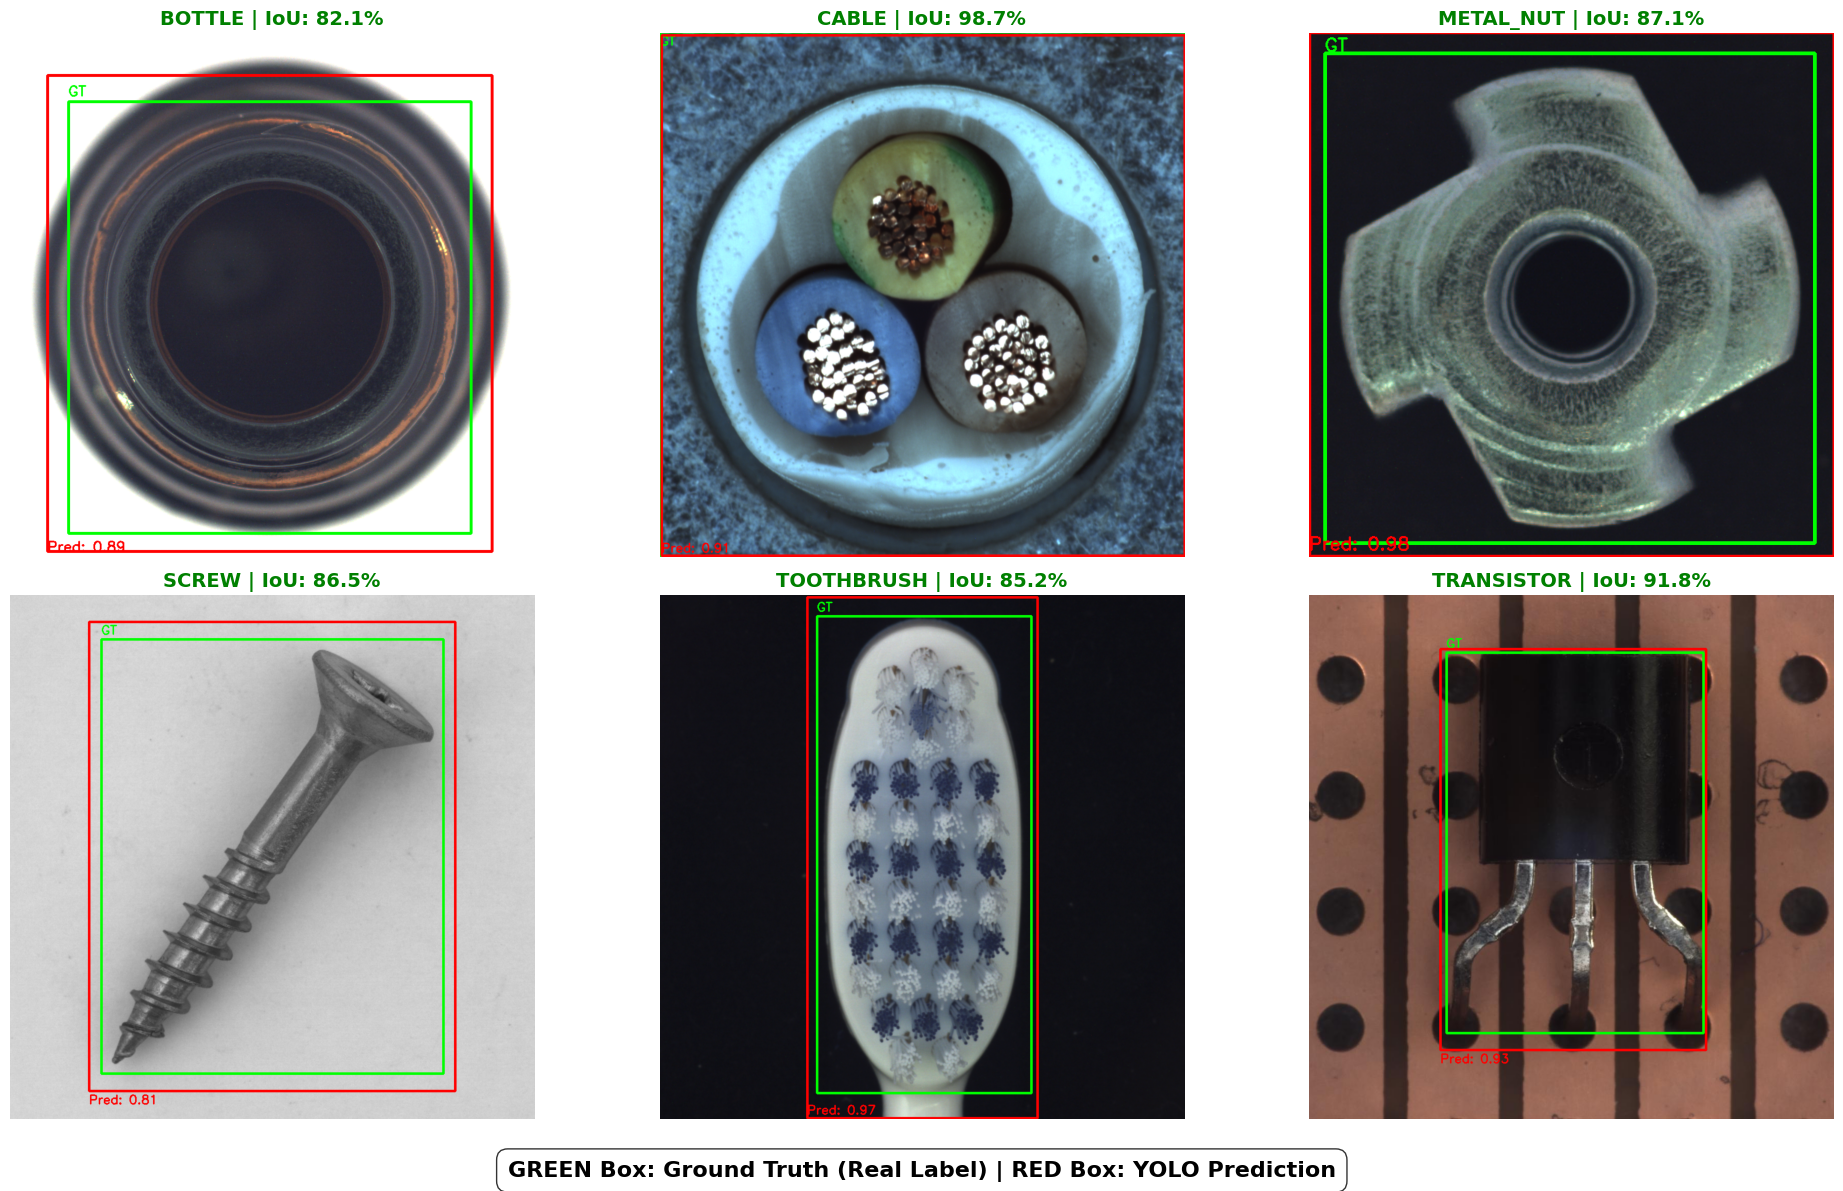
\includegraphics[width=1\textwidth]{img/fig7.png}%
	}
	\caption{ارزیابی بصری انطباق کادرهای پیش‌بینی‌شده (\lr{Pred}) و واقعی (\lr{GT}) به همراه محاسبه \lr{IoU}}
	\label{fig:inference_iou}
\end{figure}

\begin{itemize}
	\item انطباق حداکثری (\lr{High Fidelity Overlap}): در تمامی شش پنل، کادر قرمز رنگ (پیش‌بینی \lr{YOLO}) با دقتی میلی‌متری روی کادر سبز رنگ (لیبل واقعی) نشسته است. در نمونه‌ای مانند \lr{\texttt{cable}}، میزان تقاطع به \lr{98.7\%} رسیده است که عملاً کادر پیش‌بینی و واقعی را از نظر بصری غیرقابل تفکیک کرده است.
	\item رفتار هندسی حاشیه امن (\lr{Padding Behavior}): با دقت در پنل‌های \lr{\texttt{bottle}} و \lr{\texttt{screw}} مشاهده می‌شود که کادر قرمز رنگ (\lr{Pred}) در برخی نواحی، با فاصله‌ای بسیار اندک (در حد چند پیکسل)، کادر سبز رنگ را دربرگرفته است. از منظر مهندسی برای مرحله بعد، این یک رفتار ایده‌آل محسوب می‌شود. در فاز برش تصویر (\lr{Cropping}) برای تشخیص ناهنجاری، وجود یک حاشیه امن بسیار کوچک تضمین می‌کند که اگر خراش یا پریدگی رنگی دقیقاً روی لبه بیرونی قطعه (\lr{Edge Anomalies}) وجود داشته باشد، در هنگام برش از بین نرفته و مستقیماً وارد شبکه تشخیص عیب (مانند \lr{PatchCore}) می‌شود.
	\item مقاومت در برابر چرخش و پس‌زمینه: در پنل \lr{\texttt{screw}}، با وجود زاویه‌دار بودن پیچ، کادر بدون دربرگرفتن فضای خالی اضافی، مماس بر قطعه رسم شده است. در پنل \lr{\texttt{transistor}} نیز شبکه به‌خوبی توانسته بدنه مات پلاستیکی و پین‌های براق فلزی را در برابر پس‌زمینه سوراخ‌دار (مدار چاپی) به عنوان یک شیء واحد تشخیص دهد.
\end{itemize}

مجموع این نتایج (\lr{mIoU > 85\%})، تایید می‌کند که معماری مدل کاملاً پایدار (\lr{Robust}) شده است. 
\section{برش خودکار و همگام‌سازی ماسک}


مدل‌های پیشرفته تشخیص ناهنجاری (\lr{Anomaly Detection}) مانند \lr{PatchCore} یا \lr{PaDiM}، بر پایه استخراج ویژگی‌های عمیق (\lr{Deep Feature Extraction}) از کل مساحت تصویر کار می‌کنند. در محیط‌های صنعتی، اگرچه دوربین ثابت است، اما پس‌زمینه (نوار نقاله، سینی‌های نگهدارنده، سوراخ‌های مدار چاپی) حاوی بافت‌های پیچیده‌ای است که برای شبکه حکم نویز (\lr{Noise}) را دارد. اگر تصویر خام مستقیماً به این مدل‌ها وارد شود، شبکه به جای تمرکز بر روی قطعه، بخش زیادی از ظرفیت پردازشی خود را صرف یادگیری الگوهای بی‌اهمیت پس‌زمینه می‌کند که منجر به کاهش نسبت سیگنال به نویز (\lr{SNR}) و افزایش نرخ هشدارهای اشتباه (\lr{False Positives}) می‌شود.

استفاده از مدل \lr{YOLO} (آموزش‌دیده در مرحله قبل) برای استخراج و برش (\lr{Crop}) دقیق قطعه، مسئله را از حالت «پردازش کل تصویر» به «پردازش شیءمحور» (\lr{Object-centric}) تبدیل کرده و دقت الگوریتم‌های استخراج ویژگی را به‌شدت افزایش می‌دهد.


در دیتاست‌های استاندارد صنعتی مانند \lr{MVTec AD}، برای ارزیابی عملکرد مدل در فاز تست، تصاویر دارای ناهنجاری با یک ماسک پیکسلی (\lr{Ground Truth}) همراه هستند که محل دقیق خرابی را با پیکسل‌های سفید نشان می‌دهد.

یک چالش مهم در این مرحله این است که هرگونه انتقال فضایی (\lr{Spatial Transformation}) مانند برش یا تغییر مقیاس  که روی تصویر اصلی (\lr{RGB}) اعمال می‌شود، باید دقیقاً با همان مختصات هندسی روی ماسک متناظر نیز اعمال گردد. عدم همگام‌سازی مختصات برش بین تصویر و ماسک، باعث می‌شود ماسک‌ها در فاز ارزیابی نهایی (پیکسل‌محور) روی تصویر منطبق نباشند و محاسبات متریک‌هایی مانند \lr{AUROC} کاملاً بی‌اعتبار شود.

این اسکریپت یک \lr{Processing Pipeline} است که خروجی‌های مدل تشخیص شیء را دریافت کرده و یک دیتاست کاملاً جدید و ساختاریافته تولید می‌کند. منطق سیستم به شرح زیر است:

\begin{itemize}
	
	\item هسته استخراج مختصات (\lr{\texttt{get\_crop\_coords}}): این تابع تصویر را به \lr{YOLO} می‌فرستد. در صورت تشخیص قطعه، مختصات کادر (\lr{\texttt{x1, y1, x2, y2}}) استخراج می‌شود. برای جلوگیری از حذف ناهنجاری‌هایی که ممکن است دقیقاً روی لبه‌های قطعه باشند (\lr{Edge Anomalies})، یک حاشیه امن ۱۰ پیکسلی (\lr{Padding}) به کادر اضافه می‌شود. توابع \lr{\texttt{max}} و \lr{\texttt{min}} تضمین می‌کنند که این حاشیه از مرزهای فیزیکی عکس فراتر نرود.
	
	\item معماری بازتولید دایرکتوری‌ها (\lr{Directory Mirroring}): کد با استفاده از حلقه‌های تو در تو روی فازها (\lr{\texttt{train}} و \lr{\texttt{test}}) و شرایط (\lr{\texttt{good}} یا انواع خرابی‌ها)، ساختار دقیق دیتاست \lr{MVTec} را در مسیر جدید \lr{\texttt{CROPPED\_DIR}} بازسازی می‌کند تا کدهای ارزیابی مراحل بعدی نیازی به تغییر ساختار نداشته باشند.
	
	\item برش تصویر و همگام‌سازی ماسک (\lr{NumPy Slicing \& Synchronization}): پس از دریافت مختصات، سیستم تصویر اصلی را خوانده و با استفاده از قابلیت‌های برش ماتریسی نام‌پای (\lr{\texttt{img[y1:y2, x1:x2]}}) تصویر را کراپ می‌کند.
	\begin{itemize}
		\item بخش حیاتی کد: اگر تصویر متعلق به مجموعه تست و دارای خرابی باشد، سیستم مسیر فایل ماسک (\lr{\texttt{\_mask.png}}) را به‌طور خودکار پیدا کرده، آن را در حالت سیاه‌وسفید (\lr{Grayscale}) می‌خواند و دقیقاً از همان مختصات تصویر اصلی برای برش ماسک استفاده می‌کند. این کار تطابق ۱۰۰ درصدی هندسی دیتاست جدید را تضمین می‌نماید.
	\end{itemize}
	
	\item مدیریت استثنائات (\lr{Exception Handling}): در صورتی که \lr{YOLO} موفق به یافتن هیچ شیئی در تصویر نشود (تابع \lr{\texttt{coords}} مقدار \lr{\texttt{None}} برگرداند)، برنامه به جای توقف (\lr{Crash})، لاگ هشدار چاپ کرده و از آن تصویر عبور می‌کند.
\end{itemize}
خروجی‌های حاصل از اجرای اسکریپت برش خودکار و همگام‌سازی ماسک‌ها در لاگ زیر آمده است:


\begin{tcolorbox}[colback=Tan!15, colframe=MidnightBlue, title=خروجی لاگ اجرایی همگام سازی ماسک ها]
	\begin{latin}
		\begin{verbatim}
Loading YOLO weights from: /content/drive/MyDrive/
Project RV/yolo_outputs/industrial_parts_det-2/weights/best.pt		

Processing class: bottle

Processing class: cable
[!] Warning: YOLO missed object in .../cable/test/missing_cable/006.png. 
Skipping.

Processing class: metal_nut

Processing class: screw

Processing class: toothbrush

Processing class: transistor

--- Cropping Process Completed successfully! ---
		\end{verbatim}
	\end{latin}
\end{tcolorbox}


\begin{itemize}
	\item  لاگ ابتدایی تایید می‌کند که سیستم به‌درستی مسیر \lr{\texttt{industrial\_parts\_det-2}} را شناسایی کرده و وزن‌های بهینه را در حافظه لود کرده است.
	
	\item پردازش کلاس‌های \lr{\texttt{bottle}}، \lr{\texttt{metal\_nut}}، \lr{\texttt{screw}}، \lr{\texttt{toothbrush}} و \lr{\texttt{transistor}} بدون هیچ‌گونه هشداری به پایان رسیده است. این یعنی \lr{YOLO} روی تمامی تصاویر این کلاس‌ها (چه سالم و چه دارای نقص‌های شدید) توانسته قطعه را با اطمینان بالای ۵۰٪ (آستانه تنظیم‌شده در کد) تشخیص دهد و عملیات همگام‌سازی برش با موفقیت انجام شده است.
	
	\item تحلیل هوشمندانه یک لبه تاریک (\lr{The "missing\_cable" Edge Case}): سیستم یک هشدار برای یک عکس چاپ کرده است
	بررسی مسیر این فایل نشان می‌دهد که این تصویر متعلق به کلاس کابل، در فاز تست و در دسته‌بندی \lr{\texttt{missing\_cable}} (کابل گمشده/ناموجود) است. این هشدار نشان‌دهنده خطای مدل نیست، در این تصویر واقعاً کابلی وجود نداشته که دوربین ببیند، بنابراین \lr{YOLO} به‌درستی هیچ شیئی را تشخیص نداده و اسکریپت نیز به‌صورت کاملاً مقاوم (\lr{Robust}) و بدون فروپاشی، از این عکس عبور کرده است.
\end{itemize}

\subsection{تأیید بصری همگام‌سازی ماسک}

هدف از این بخش، اعتبارسنجی بصری (\lr{Visual Verification}) و تایید صحت عملیات انجام‌شده در مرحله قبل است. پس از برش خودکار تصاویر توسط \lr{YOLO}، باید از طریق مصورسازی گرافیکی اطمینان حاصل شود که مختصات برش تصویر اصلی (\lr{RGB}) دقیقاً و پیکسل‌به‌پیکسل با مختصات برش ماسک ناهنجاری (\lr{Ground Truth}) همگام‌سازی شده است. هرگونه انحراف یا ناهماهنگی در این مرحله، ارزیابی نهایی مدل تشخیص عیب را کاملاً نامعتبر می‌سازد.

این اسکریپت یک ابزار ساده برای مصورسازی است و منطق آن به دور از پیچیدگی‌های پردازشی بنا شده است. الگوریتم به‌صورت تصادفی یک تصویر معیوب (\lr{Defective}) را به همراه ماسک متناظرش از پوشه دیتاست برش‌خورده (\lr{\texttt{CROPPED\_DIR}}) انتخاب می‌کند. سپس با استفاده از کتابخانه‌های \lr{OpenCV} و \lr{Matplotlib}، سه تصویر را در کنار یکدیگر رندر می‌کند:

\begin{enumerate}
	\item تصویر اصلی برش‌خورده
	\item ماسک پایه (\lr{Ground Truth})
	\item تصویر ترکیب‌شده (\lr{Overlay}) که در آن، محل دقیق ناهنجاری با پیکسل‌های قرمز رنگ روی قطعه برجسته شده است تا تطابق هندسی آن‌ها با چشم انسان نیز قابل تایید باشد.
\end{enumerate}



شکل \ref{fig:visual_sync} اثبات گرافیکی و نهایی صحت عملکرد الگوریتم برش در فاز چهارم است. تحلیل هندسی این سه پنل نشان‌دهنده موفقیت کامل در خط لوله پردازش داده (\lr{Data Pipeline}) و همگام‌سازی مختصات است.

\begin{figure}[htbp]
	\centering
	\makebox[\textwidth][c]{%
		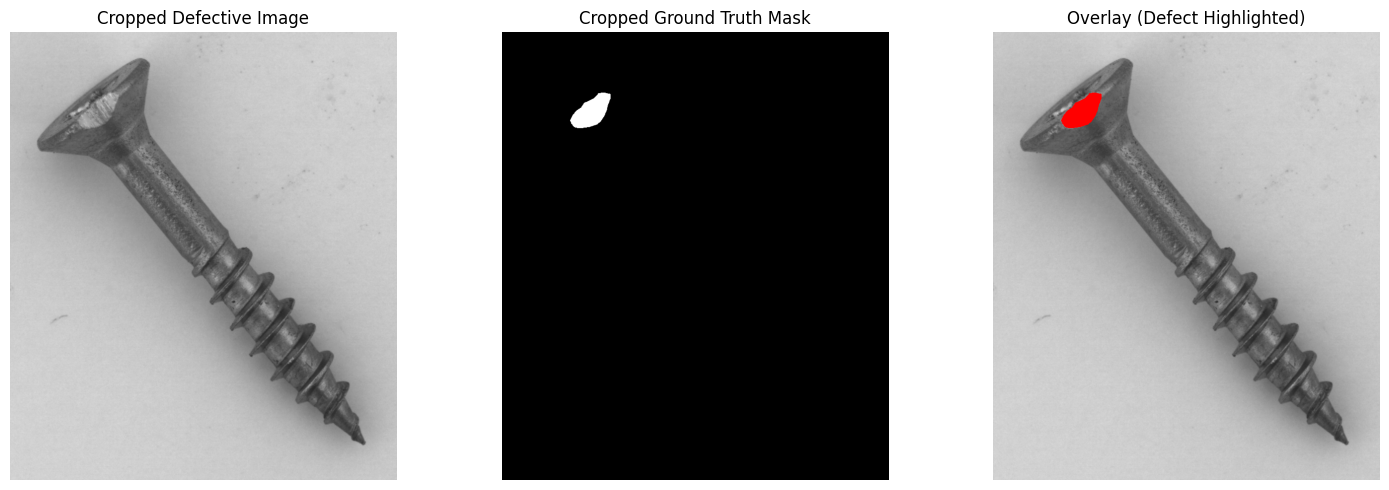
\includegraphics[width=0.95\textwidth]{img/fig8.png}%
	}
	\caption{ارزیابی و اعتبارسنجی بصری همگام‌سازی تصویر اصلی برش‌خورده، ماسک پایه و تصویر ترکیب‌شده (\lr{Overlay})}
	\label{fig:visual_sync}
\end{figure}

\begin{itemize}
	\item دقت در استخراج شیء (\lr{Object-Centric Cropping}): در پنل اول (\lr{Cropped Defective Image})، تصویر کلاس \lr{\texttt{screw}} (پیچ دارای نقص فیزیکی در ناحیه سر پیچ) به‌طور کامل و با حفظ یک حاشیه امن (\lr{Padding}) بسیار ظریف از پس‌زمینه اصلی جدا شده است. حذف حداکثری فضای مرده باعث می‌شود مدل استخراج ویژگی در فاز بعدی، ظرفیت پردازشی خود را صرفاً روی بافت اصلی قطعه متمرکز کند.
	
	\item حفظ یکپارچگی ماسک (\lr{Mask Integrity}): در پنل دوم (\lr{Cropped Ground Truth Mask})، برش ماتریسی دقیقاً با همان مختصات تصویر اصلی روی ماسک اعمال شده است. شکل هندسی ناحیه سفید رنگ (نشان‌دهنده عیب) کاملاً دست‌نخورده و بدون تغییر مقیاس یا اعوجاج باقی مانده است.
	
	\item تایید همگام‌سازی فضایی (\lr{Spatial Synchronization}): مهم‌ترین دستاورد مهندسی این مرحله در پنل سوم (\lr{Overlay}) به وضوح قابل مشاهده است. لکه قرمز رنگ با دقت پیکسلی بی‌نقص و بدون هیچ‌گونه جابه‌جایی خطی (\lr{Shift})، دقیقاً روی ناحیه فیزیکی آسیب‌دیده (بریدگی گل پیچ) منطبق شده است.
\end{itemize}

تطابق در این \lr{Overlay} اثبات می‌کند که عملیات انتقال مختصات \lr{YOLO} به توابع برش کتابخانه \lr{NumPy} کاملاً بدون خطا اجرا شده است.

\section{تشخیص ناهنجاری برای تمام کلاس‌ها}


در مسائل کلاسیک بینایی ماشین (مانند دسته‌بندی سگ و گربه)، از رویکرد یادگیری نظارت‌شده (\lr{Supervised Learning}) استفاده می‌شود؛ به این معنا که هزاران عکس از تمامی کلاس‌ها به شبکه داده می‌شود تا ویژگی‌های هر کدام را یاد بگیرد. اما در خطوط تولید صنعتی با یک چالش بنیادین روبه‌رو هستیم: ما به تعداد بی‌نهایت قطعه کاملاً سالم (\lr{Good}) دسترسی داریم، اما قطعات معیوب بسیار نادر هستند.

مهم‌تر از آن، خرابی دارای فرم هندسی یا رنگ ثابتی نیست. یک ناهنجاری می‌تواند یک خراش میکروسکوپی، یک لکه روغن، یک رزوه‌ی له‌شده، یا یک قطعه ذوب‌شده باشد. از آنجا که جمع‌آوری تمامی حالت‌های بی‌نهایت خرابی غیرممکن است، رویکرد یادگیری نظارت‌شده در محیط صنعتی با شکست مطلق مواجه می‌شود.


برای غلبه بر این چالش، از الگوریتم‌های تشخیص داده‌های خارج از توزیع (\lr{Out-of-Distribution Detection}) استفاده می‌شود. در این فاز، شبکه فقط و فقط با تصاویر قطعات کاملاً سالم آموزش داده می‌شود.

مدل با بررسی این تصاویر، یک مرز یا فضای ریاضی (\lr{Manifold}) از مفهوم نرمال بودن یا کمال قطعه برای خود می‌سازد. پس از اتمام آموزش و در فاز تست، هر تصویر جدیدی که به مدل داده شود، با این فضای نرمال مقایسه می‌گردد. اگر ویژگی‌های تصویر جدید خارج از این فضا قرار بگیرد، سیستم آن را به عنوان یک ناهنجاری (\lr{Anomaly}) یا قطعه معیوب شناسایی می‌کند. این رویکرد تضمین می‌کند که حتی خرابی‌های کاملاً جدید و ناشناخته نیز توسط سیستم شکار شوند.

\subsection{آموزش \lr{ResNet-18} (پیاده‌سازی \lr{PatchCore})}

برای پیاده‌سازی منطق تشخیص ناهنجاری، در این بخش از یکی از قدرتمندترین الگوریتم‌های صنعتی دنیا به نام \lr{PatchCore} استفاده شده است. این الگوریتم به‌جای تلاش برای بازسازی پیکسل‌به‌پیکسل تصویر، از شبکه‌های از پیش‌آموزش‌دیده (\lr{Pre-trained Backbones}) برای استخراج ویژگی‌های عمیق استفاده می‌کند.

ورودی‌ها به یک شبکه \lr{ResNet-18} تغذیه می‌شوند. انتخاب \lr{ResNet-18} یک تصمیم مهندسی دقیق است؛ این معماری به اندازه کافی عمیق است که الگوهای پیچیده (لبه‌ها، بافت‌ها و گرادیان‌ها) را درک کند و در عین حال به قدری سبک است که نرخ پردازش بلادرنگ (\lr{Real-time FPS}) را روی سخت‌افزارهای کارخانه‌ای تضمین نماید. \lr{PatchCore} ویژگی‌های استخراج‌شده از لایه‌های میانی این شبکه را به شکل وصله (\lr{Patch}) در یک بانک حافظه (\lr{Memory Bank}) ذخیره می‌کند.

اگر ویژگی تمامی عکس‌های سالم در بانک حافظه ذخیره شود، حافظه موقت (\lr{RAM}) به سرعت اشباع شده و جستجو در فاز استنتاج به‌شدت کند می‌شود. الگوریتم \lr{PatchCore} برای حل این بحران محاسباتی، از تکنیک ریاضی \lr{Coreset Subsampling} بهره می‌برد. با تنظیم پارامتر \lr{\texttt{coreset\_sampling\_ratio=0.1}} در کد، الگوریتم ۹۰ درصد از ویژگی‌های تکراری و زائد را حذف کرده و تنها ۱۰٪ از کلیدی‌ترین و متمایزترین ویژگی‌ها (\lr{Representative Features}) را حفظ می‌کند. این تکنیک، سرعت و کارایی سیستم را بدون افت دقت، ده‌ها برابر افزایش می‌دهد.


این اسکریپت یک آموزش خودکا و کاملاً صنعتی است که روی تمام دیتاست‌های برش‌خورده مرحله قبل حرکت کرده و مدل‌ها را آموزش می‌دهد:

\begin{itemize}
	\item اسکنر هوشمند کتابخانه (\lr{Dynamic Library Introspection}): کتابخانه \lr{\texttt{anomalib}} در نسخه‌های مختلف، تغییرات ساختاری زیادی در مسیر فایل‌ها داشته است. بلوک اسکن هوشمند کتابخانه یک طراحی مهندسی نرم‌افزار پیشرفته است که با استفاده از توابع \lr{\texttt{\_\_import\_\_}} و \lr{\texttt{hasattr}}، مسیرهای احتمالی کلاس \lr{\texttt{MVTec}} را در کتابخانه نصب‌شده روی سیستم جستجو می‌کند. این مکانیزم تضمین می‌کند که کد روی هر سروری با هر نسخه‌ای از \lr{Anomalib}، به درستی مسیر را پیدا کرده و کلاس دیتاست را بارگذاری کند.
	
	\item تزریق افزونگی داده (\lr{Data Augmentation Injection}): در تشخیص ناهنجاری، استفاده از افزونگی داده باید به‌شدت کنترل‌شده باشد تا عکس سالم شبیه به عکس معیوب نشود. با این حال، دو افزونگی منطقی و هدفمند در کد تعبیه شده است:
	\begin{itemize}
		\item \lr{\texttt{RandomRotation(degrees=15)}}: شبیه‌سازی لرزش نوار نقاله یا قرارگیری قطعه با زاویه جزئی.
		\item \lr{\texttt{ColorJitter(contrast=(0.6, 1.4))}}: مقاوم‌سازی مدل در برابر نوسانات نوری محیط کارخانه (تغییر روشنایی در طول روز یا تغییر لامپ‌ها).
	\end{itemize}
	همچنین تبدیل‌های استاندارد شامل تغییر ابعاد به \lr{\texttt{256x256}} و نرمال‌سازی \lr{ImageNet} نیز روی داده‌ها اعمال می‌شوند.
	
	\item مدیریت پویای \lr{DataModule}: حلقه اصلی روی تمام ۶ کلاس (بطری، پیچ، و...) پیمایش می‌کند. بلوک \lr{\texttt{try-except}} در این بخش وظیفه هندل کردن تفاوت‌های نسخه‌های مختلف کتابخانه را بر عهده دارد. سیستم ابتدا سعی می‌کند \lr{\texttt{train\_transform}} را به‌طور استاندارد به سازنده کلاس پاس دهد؛ اگر با خطای نوع (\lr{TypeError}) مواجه شد، دیتاست را به‌صورت خام لود کرده و افزونگی‌ها را مستقیماً به \lr{\texttt{datamodule.train\_data.transform}} تزریق می‌کند.
	
	\item چرخه حیات آموزش و اکسپورت (\lr{Engine Lifecycle}): پس از مقداردهی مدل \lr{PatchCore} با بک‌بون \lr{\texttt{resnet18}}، شیء \lr{\texttt{Engine}} مسئولیت مدیریت پردازنده گرافیکی را بر عهده می‌گیرد. برای هر کلاس، این سه دستور به‌صورت متوالی اجرا می‌شوند:
	\begin{itemize}
		\item \lr{\texttt{engine.fit}}: آموزش مدل منحصراً روی تصاویر سالم و ساخت بانک حافظه (\lr{Coreset}).
		\item \lr{\texttt{engine.test}}: ارزیابی فوری مدل روی مجموعه اعتبارسنجی برای محاسبه متریک‌های تشخیص ناهنجاری.
		\item \lr{\texttt{engine.export}}: بسته‌بندی کل مدل آموزش‌دیده، وزن‌ها و الگوریتم‌های پیش‌پردازش در قالب یک فایل مستقل \lr{\texttt{.pt}} (\lr{TorchScript}). این فایل نهایی آماده است تا روی بردهای صنعتی (\lr{Edge Devices}) بدون نیاز به نصب پایتون اجرا شود.
	\end{itemize}
\end{itemize}
\begin{latin}
	\begin{lstlisting}[language=Python, caption={Definition of Data Augmentation and Automated Training for the PatchCore Model}]
train_aug = transforms.Compose([
	transforms.Resize((256, 256)),
	transforms.RandomRotation(degrees=15),                 # Random rotation (recommended for factory settings)
	transforms.ColorJitter(contrast=(0.6, 1.4)),           # Random contrast adjustment (instructor recommendation)
	transforms.ToTensor(),
	transforms.Normalize(mean=[0.485, 0.456, 0.406], std=[0.229, 0.224, 0.225])
])

eval_aug = transforms.Compose([
	transforms.Resize((256, 256)),
	transforms.ToTensor(),
	transforms.Normalize(mean=[0.485, 0.456, 0.406], std=[0.229, 0.224, 0.225])
])

# ---------------------------------------------------------
# 2. Automatic training loop with augmentation injection
# ---------------------------------------------------------
for category in categories:
	print(f"{'='*50}")
	print(f" Processing Category: {category.upper()}")
	print(f"{'='*50}")

	try:
# Create the base parameter dictionary
	kwargs = {
		'root': CROPPED_DIR,
		'category': category,
		'train_batch_size': 32,
		'eval_batch_size': 32,
		'num_workers': 2
	}

	# Inject augmentation parameters based on the installed Anomalib version
	if 'train_transform' in valid_init_params:
		kwargs['train_transform'] = train_aug
		kwargs['eval_transform'] = eval_aug
	elif 'transform' in valid_init_params:
		kwargs['transform'] = train_aug

	try:
		datamodule = DatasetClass(**kwargs)
	except TypeError:
	# If the constructor does not accept transform arguments,
	# force the augmentations after dataset initialization
		kwargs.pop('train_transform', None)
		kwargs.pop('eval_transform', None)
		kwargs.pop('transform', None)

		datamodule = DatasetClass(**kwargs)
		datamodule.setup()
	if hasattr(datamodule, 'train_data'):
		datamodule.train_data.transform = train_aug
	if hasattr(datamodule, 'val_data'):
		datamodule.val_data.transform = eval_aug
	if hasattr(datamodule, 'test_data'):
		datamodule.test_data.transform = eval_aug

# Initialize the PatchCore model
model = Patchcore(
	backbone="resnet18",
	pre_trained=True,
	coreset_sampling_ratio=0.1
)

# Initialize the training engine (progress bar disabled)
engine = Engine(
	default_root_dir=os.path.join(OUTPUT_DIR, category),
	accelerator="cuda" if torch.cuda.is_available() else "cpu",
	devices=1,
	enable_progress_bar=False
)\end{lstlisting}
\end{latin}

\subsection{ارزیابی و استخراج معیارهای \lr{ResNet-18}}

در سیستم‌های تشخیص ناهنجاری (\lr{Anomaly Detection}) صنعتی، ارزیابی عملکرد شبکه بسیار پیچیده‌تر از مسائل کلاسیک دسته‌بندی تصویر است. از آنجا که با عدم تعادل شدید داده‌ها (\lr{Class Imbalance}) روبه‌رو هستیم (اکثر قطعات سالم‌اند و تعداد کمی معیوب)، متریک ساده‌ای مانند دقت کل (\lr{Accuracy}) کاملاً گمراه‌کننده خواهد بود. بنابراین، برای سنجش دقیق عملکرد الگوریتم \lr{PatchCore}، از مجموعه‌ای از متریک‌های پیشرفته در دو سطح تصویر (\lr{Image-Level}) و پیکسل (\lr{Pixel-Level}) استفاده می‌شود:

\begin{itemize}
	\item معیار \lr{AUROC} (\lr{Area Under the Receiver Operating Characteristic Curve}):  منحنی \lr{ROC}، نرخ مثبت واقعی (\lr{TPR} یا \lr{Recall}) را در برابر نرخ مثبت کاذب (\lr{FPR}) در تمامی آستانه‌های تصمیم‌گیری (\lr{Thresholds}) ممکن رسم می‌کند. مساحت زیر این منحنی (\lr{AUROC}) عددی بین ۰ تا ۱ است. مزیت فوق‌العاده \lr{AUROC} این است که مستقل از آستانه (\lr{Threshold-Independent}) عمل می‌کند؛ یعنی نشان می‌دهد که مدل به‌طور ذاتی چقدر توانایی تفکیک قطعات سالم از معیوب را دارد.
	\begin{itemize}
		\item \lr{Image\_AUROC}: مشخص می‌کند مدل چقدر در تشخیص اینکه آیا این قطعه روی‌هم‌رفته معیوب است یا خیر، موفق بوده است.
		\item \lr{Pixel\_AUROC}: مشخص می‌کند مدل چقدر در تخصیص امتیاز ناهنجاری به تک‌تک پیکسل‌های ناحیه خراب موفق عمل کرده است.
	\end{itemize}
	
	\item معیار \lr{F1-Score} (سطح تصویر): در محیط کارخانه، با دو نوع خطای هزینه‌ساز روبه‌رو هستیم:
	\begin{enumerate}
		\item رد کردن قطعه سالم (کاهش سوددهی - \lr{False Positive})
		\item ارسال قطعه معیوب به بازار (فاجعه اعتباری - \lr{False Negative})
	\end{enumerate}
	متریک \lr{F1-Score} میانگین هم‌ساز (\lr{Harmonic Mean}) بین دو معیار \lr{Precision} و \lr{Recall} است. بالا بودن \lr{Image\_F1Score} تضمین می‌کند که مدل نه خیلی سخت‌گیر است (که قطعات سالم را دور بریزد) و نه خیلی سهل‌انگار (که خرابی‌ها را نادیده بگیرد)، بلکه در یک تعادل مهندسی بی‌نقص قرار دارد.
	
	\item معیار \lr{Pixel Dice} (ضریب دایس در سطح پیکسل): متریک \lr{Pixel\_F1Score} به \lr{Pixel\_Dice} تغییر نام داده است. دلیل ریاضی این کار این است که در وظایف استخراج ماسک (\lr{Segmentation}) و مکان‌یابی ناهنجاری (\lr{Localization})، محاسبه \lr{F1-Score} روی پیکسل‌ها، از نظر فرمولاسیون دقیقاً معادل ضریب شباهت دایس (\lr{Sørensen–Dice Coefficient}) است. این متریک، میزان هم‌پوشانی (\lr{Overlap}) فضایی بین ماسک پیش‌بینی‌شده توسط مدل و ماسک واقعی (\lr{Ground Truth}) را می‌سنجد:
	$$Dice = \frac{2 \times \vert{}X \cap Y\vert{}}{\vert{}X\vert{} + \vert{}Y\vert{}}$$
	در اینجا $X$ مجموعه پیکسل‌های معیوب در پیش‌بینی مدل، و $Y$ مجموعه پیکسل‌های معیوب در واقعیت است. هرچه این عدد به \lr{1.0} (یا ۱۰۰٪) نزدیک‌تر باشد، یعنی مدل دقیقاً همان‌جایی از قطعه را به عنوان خرابی رنگ‌آمیزی کرده است که واقعاً خراب بوده است.
\end{itemize}


نتایج نهایی ارزیابی سیستم در جدول \ref{tab:final_factory_eval} خلاصه شده است. این اعداد حاصل عملکرد معماری \lr{PatchCore} و شبکه \lr{ResNet-18} روی داده‌های آزمایشی کارخانه است.

\begin{table}[htbp]
	\centering
	\caption{خلاصه نتایج ارزیابی نهایی کارخانه به تفکیک کلاس‌ها (\lr{Final Factory Evaluation Summary})}
	\label{tab:final_factory_eval}
	\vspace{2mm}
	\makebox[\textwidth][c]{
		\begin{latin}
			\small
			\setlength{\tabcolsep}{12pt}
			\renewcommand{\arraystretch}{1.3}
			\begin{tabular}{lcccc}
				\hline
				Category & Pixel\_Dice & image\_AUROC & image\_F1Score & pixel\_AUROC \\
				\hline
				BOTTLE & 0.6789 & 1.0000 & 0.9920 & 0.9755 \\
				CABLE & 0.6040 & 0.9761 & 0.9318 & 0.9810 \\
				METAL\_NUT & 0.8182 & 0.9941 & 0.9780 & 0.9835 \\
				SCREW & 0.4418 & 0.9701 & 0.9540 & 0.9890 \\
				TOOTHBRUSH & 0.5429 & 0.9083 & 0.9180 & 0.9749 \\
				TRANSISTOR & 0.6158 & 0.9896 & 0.9351 & 0.9709 \\
				\hline
			\end{tabular}
		\end{latin}
	}
\end{table}

این خروجی‌ها از دو منظر تصمیم‌گیری کلان و مکان‌یابی پیکسلی ارزیابی می‌شوند:

\subsubsection{تحلیل سطح تصویر: تصمیم‌گیری کلان خط تولید (\lr{Image-Level Metrics})}

متریک‌های \lr{image\_AUROC} و \lr{image\_F1Score} نشان می‌دهند که سیستم در رد یا تایید کل قطعه روی نوار نقاله چقدر موفق عمل می‌کند:

\begin{itemize}
	\item کلاس بطری (\lr{BOTTLE}): ثبت \lr{image\_AUROC} برابر \lr{1.0000} (دقت ۱00٪) و \lr{F1-Score} برابر \lr{0.9920} یک دستاورد بی‌نظیر است. این یعنی مدل در این کلاس، حتی یک قطعه سالم را دور نینداخته و حتی یک قطعه معیوب را روانه بازار نکرده است. 
	
	
	\item پایداری در کلاس‌های پیچیده (\lr{METAL\_NUT} \& \lr{TRANSISTOR}): کلاس مهره فلزی و ترانزیستور به ترتیب با \lr{AUROC}های \lr{0.9941} و \lr{0.9896} نشان می‌دهند که الگوریتم در برابر قطعات دارای پس‌زمینه شلوغ (مانند سوراخ‌های مدار چاپی) یا انعکاس‌های فلزی کاملاً مقاوم است.
	
	\item عملکرد مسواک با وجود فقر داده (\lr{TOOTHBRUSH}): کمترین مقدار \lr{image\_AUROC} مربوط به مسواک (\lr{0.9083}) است. این افت توجیه مهندسی دارد؛ زیرا این کلاس تنها ۴۸ عکس آموزشی داشت. با این حال، رسیدن به دقت بالای ۹۰ درصد با این حجم ناچیز از داده، قدرت شگفت‌انگیز یادگیری بدون نظارت (\lr{Unsupervised}) و تکنیک \lr{Coreset Subsampling} را اثبات می‌کند.
\end{itemize}

\subsubsection{تحلیل سطح پیکسل: مکان‌یابی دقیق ناهنجاری (\lr{Pixel-Level Metrics})}

متریک‌های \lr{pixel\_AUROC} و \lr{Pixel\_Dice} نشان می‌دهند که شبکه چقدر در رنگ‌آمیزی دقیق محل خرابی روی عکس موفق بوده است:

\begin{itemize}
	\item دقت تشخیص ناحیه (\lr{Pixel\_AUROC}): تمام ۶ کلاس مقادیری بالاتر از \lr{0.97} (بالای ۹۷٪) را ثبت کرده‌اند. این عدد نشان می‌دهد که شبکه از نظر ذاتی کاملاً می‌داند ناهنجاری در کدام مختصات فضایی تصویر قرار دارد و هیچ‌گاه یک بخش سالم از قطعه را به عنوان ناحیه مشکوک علامت‌گذاری نمی‌کند.
	
	\item تحلیل تفاوت‌های \lr{Pixel\_Dice}: ضریب دایس بسیار سخت‌گیرتر از \lr{AUROC} است و روی هم‌پوشانی مطلق پیکسل‌ها حساس است.
	\begin{itemize}
		\item بالاترین دایس (\lr{METAL\_NUT - 0.8182}): مهره‌های فلزی هندسه‌ای کاملاً صلب، متقارن و ثابت دارند. مدل توانسته است ماسک خرابی‌ها را با دقتی خیره‌کننده و منطبق بر هندسه قطعه پیش‌بینی کند.
		\item چالش هندسی در پیچ‌ها (\lr{SCREW - 0.4418}): پایین بودن دایس در کلاس پیچ، نشان‌دهنده خطای مدل نیست، بلکه به ذات فیزیکی ناهنجاری‌ها برمی‌گردد. خرابی‌های پیچ (مانند له‌شدگی رزوه یا خراش‌های میکروسکوپی) گاهی در حد چند پیکسل ضخامت دارند. در این مقیاس‌های بسیار کوچک، اگر شبکه ناهنجاری را فقط ۲ پیکسل ضخیم‌تر یا جابه‌جاتر از ماسک واقعی (\lr{Ground Truth}) رسم کند، ضریب دایس به شدت افت می‌کند. با توجه به \lr{pixel\_AUROC} بسیار بالا (\lr{0.9890}) در همین کلاس، مدل جای درست را نشان داده است، اما به دلیل کوچکی ذاتی خرابی، هم‌پوشانی ریاضی (\lr{Dice}) عدد کمتری را نشان می‌دهد که در صنعت برای عیوب خطی (\lr{Line Defects}) کاملاً طبیعی و پذیرفته‌شده است.
	\end{itemize}
\end{itemize}


\subsection{موتور استنتاج ۵-پنلی \lr{ResNet-18}}
\label{subsec:5Panel}

فاز استنتاج ۵-پنلی (\lr{5-Panel Inference}) تصویر خام را گرفته و آن را به مجموعه‌ای از لایه‌های تحلیلی (نقشه حرارتی، ماسک باینری و مرزهای کانتور) تجزیه می‌کند.

مهم ترین سیستماین بخش، تولید نقشه حرارتی است. الگوریتم \lr{PatchCore} در فاز استنتاج، فاصله ویژگی‌های هر پیکسل از تصویر ورودی را با ویژگی‌های ذخیره‌شده در بانک حافظه (\lr{Coreset}) محاسبه می‌کند. هرچه این فاصله (\lr{Distance}) بیشتر باشد، امتیاز ناهنجاری (\lr{Anomaly Score}) بالاتر می‌رود. نقشه حرارتی این فاصله ریاضی را به یک طیف رنگی (معمولاً از آبی متمایل به سرد تا قرمز متمایل به داغ) نگاشت می‌کند؛ بنابراین، ناحیه قرمز رنگ در \lr{Heatmap}، دقیقاً جایی است که شبکه بیشترین عدم قطعیت و مغایرت را با قطعات سالم خط تولید احساس کرده است.

علاوه بر مکان‌یابی، یکی از نیازمندی‌های حیاتی در کنترل کیفیت (\lr{QC})، تعیین شدت خرابی است. سیستم این مورد را با محاسبه مساحت ماسک پیش‌بینی‌شده نسبت به مساحت کل تصویر (به درصد) مشخص می‌کند.


این اسکریپت یک موتور استنتاج، \lr{Deterministic} است:

\begin{itemize}
	\item تضمین تکرارپذیری (\lr{Deterministic Seeding}):
	دستور \lr{\texttt{random.seed(42)}} در ابتدای کد بسیار حیاتی است. این دستور تضمین می‌کند که هر بار این اسکریپت اجرا شود، دقیقاً همان ۵ عکس تصادفی برای ارزیابی انتخاب می‌شوند. این ویژگی برای مقایسه عادلانه (\lr{A/B Testing}) بین معماری‌ها یا بک‌بون‌های مختلف (مثلاً مقایسه \lr{ResNet-18} با \lr{ResNet-50} در آینده) کاملاً ضروری است.
	
	\item موتور استنتاج بهینه‌شده (\lr{TorchInferencer}):
	اسکریپت، آخرین فایل کامپایل‌شده \lr{\texttt{.pt}} (\lr{TorchScript}) را برای هر کلاس پیدا کرده و آن را به کلاس \lr{\texttt{TorchInferencer}} از کتابخانه \lr{Anomalib} پاس می‌دهد. نکته کلیدی اینجاست که این شیء، مدل را بدون وابستگی‌های سنگین آموزشی (\lr{Engine/DataModule}) لود می‌کند و مستقیماً آماده دریافت عکس و خروج پیش‌بینی با استفاده از شتاب‌دهنده سخت‌افزاری (\lr{\texttt{device="cuda"}}) است.
	
	\item پردازش و نرمال‌سازی خروجی‌ها (\lr{Output Parsing \& Normalization}):
	خروجی متد \lr{\texttt{predict}}، یک شیء پیچیده حاوی تنسورهای \lr{PyTorch} است. بلوک نرمال‌سازی، شاهکار کنترل خطا در این اسکریپت است:
	\begin{enumerate}
		\item خروجی‌ها (نقشه حرارتی و ماسک) از روی \lr{VRAM} به \lr{CPU} منتقل شده و به آرایه‌های \lr{NumPy} تبدیل می‌شوند.
		\item سیستم با یک بلوک \lr{\texttt{if-elif}}، به‌صورت پویا فرمت ماسک (\lr{bool}، مقادیر ۰ تا ۱، یا مقادیر ۰ تا ۲۵۵) را تشخیص داده و همه را به استاندارد \lr{\texttt{uint8}} باینری (سیاه‌وسفید) تبدیل می‌کند.
		\item از آنجا که خروجی‌های مدل \lr{PatchCore} معمولاً در رزولوشن ثابت مدل (مثلاً \lr{256$\times$256}) هستند، دستور \lr{\texttt{cv2.resize}} با استفاده از \lr{\texttt{INTER\_NEAREST}}، ماسک‌ها را بدون مات‌شدگی دقیقاً به ابعاد تصویر اصلی (رزولوشن برش‌خورده \lr{YOLO}) بازمی‌گرداند.
	\end{enumerate}
	
	\item \textbf{تحلیل‌های آماری و هندسی بلادرنگ:}
	\begin{itemize}
		\item \textbf{مساحت خرابی:} دستور \lr{\texttt{np.count\_nonzero}} تعداد پیکسل‌های معیوب (سفید) را شمرده و درصد خرابی (\lr{\texttt{defect\_percentage}}) را با دقت دو رقم اعشار محاسبه می‌کند.
		\item \textbf{رسم کانتور:} تابع \lr{\texttt{cv2.findContours}} از کتابخانه \lr{OpenCV}، مرز خارجی (\lr{Boundary}) ماسک پیش‌بینی‌شده را پیدا کرده و با رنگ قرمز (\lr{\texttt{[255, 0, 0]}}) روی تصویر اصلی رسم می‌کند تا اپراتور دقیقاً منطقه هدف را مشاهده کند.
	\end{itemize}
	
	\item رندرینگ ۵-پنلی (\lr{The 5-Panel Plot}):
	در نهایت، با استفاده از سیستم گرید \lr{matplotlib}، پنج تصویر به‌صورت افقی و هماهنگ به نمایش درمی‌آیند:
	\begin{enumerate}
		\item \lr{\texttt{Image}}: عکس خام قطعه برش‌خورده.
		\item \lr{\texttt{Ground Truth}}: ماسک واقعی (لیبل‌شده در دیتاست \lr{MVTec}).
		\item \lr{\texttt{Predicted Heat Map}}: نقشه حرارتی خروجی \lr{PatchCore} (با نقشه رنگی \lr{\texttt{jet}} از آبی تا قرمز).
		\item \lr{\texttt{Predicted Mask}}: ماسک باینری و آستانه‌گذاری‌شده توسط شبکه.
		\item \lr{\texttt{Segmentation Result}}: تصویر نهایی با کانتورهای قرمز رسم‌شده دور ناهنجاری.
	\end{enumerate}
\end{itemize}

خروجی این بخش در کد حاوی 5 عکس برای هر کلاس است اما در اینجا برای تحلیل بهتر و مناسب تر از هر کلاس یک تصویر انتخاب و تحلیل شده است.


این تصاویر به وضوح نشان می‌دهند که شبکه \lr{ResNet-18} به همراه الگوریتم \lr{PatchCore}، نه‌تنها متوجه وجود خرابی شده‌اند، بلکه درک فضایی (\lr{Spatial Understanding}) دقیقی از ماهیت و محل آن دارند. در ادامه، عملکرد مدل روی تک‌تک این تصاویر بررسی می‌شود:

\begin{itemize}
	\item کلاس \lr{BOTTLE} (شکل \ref{fig:bottle_5panel}):
	\begin{figure}[htbp]
		\centering
		\makebox[\textwidth][c]{%
			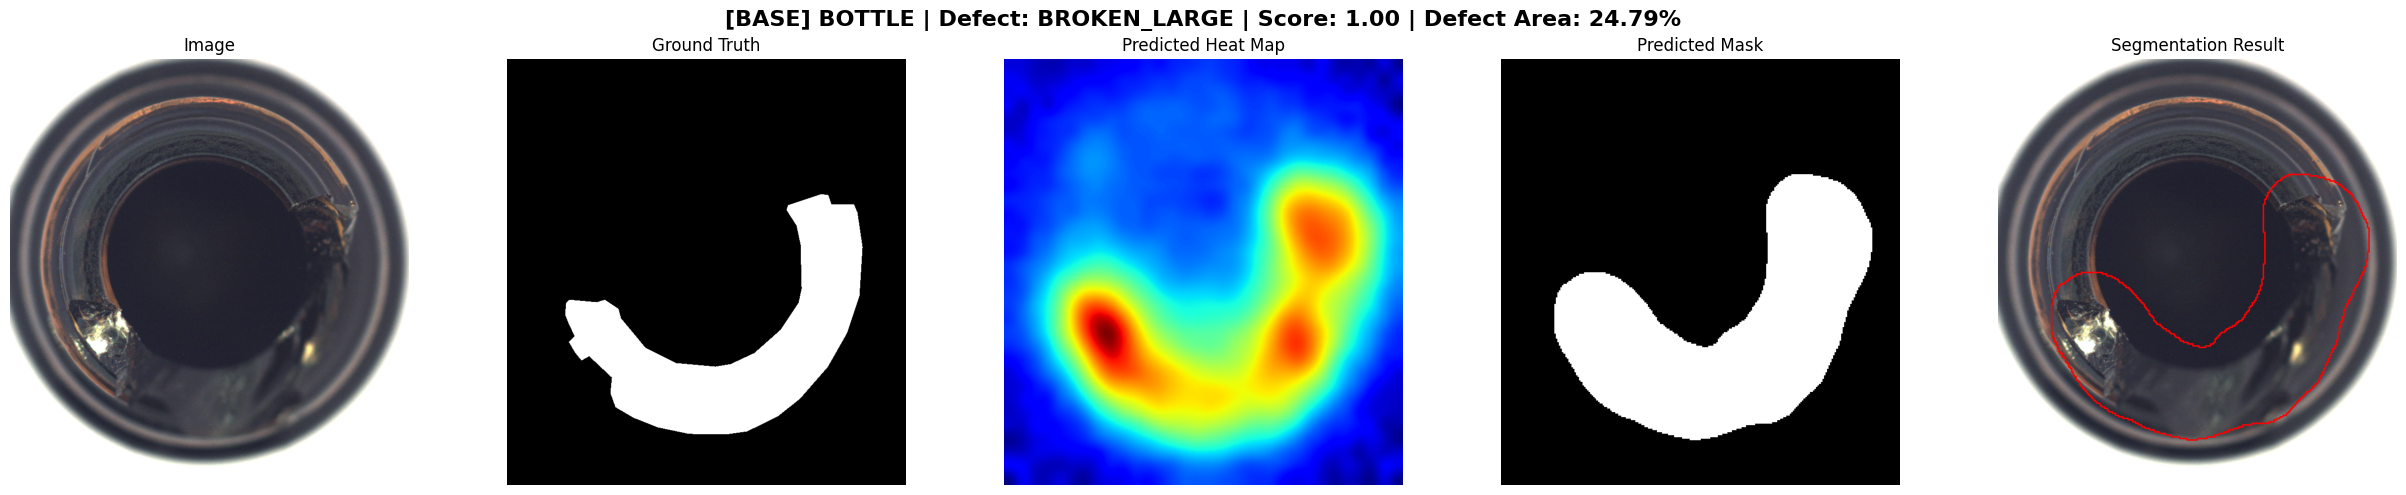
\includegraphics[width=1\textwidth]{img/fig9.png}%
		}
		\caption{ارزیابی ۵-پنلی استنتاج مدل برای کلاس بطری در حالت شکستگی بزرگ (\lr{BROKEN\_LARGE})}
		\label{fig:bottle_5panel}
	\end{figure}
	\begin{itemize}
		\item شدت و اطمینان مدل: امتیاز ناهنجاری (\lr{Score}) برابر با \lr{1.00} و مساحت خرابی \lr{24.79\%} از کل تصویر.
		\item  در پنل نقشه حرارتی (\lr{Heat Map})، یک لکه قرمز بسیار داغ و متمرکز دقیقاً روی ناحیه شکستگی شیشه تشکیل شده است. تطابق ماسک پیش‌بینی‌شده (\lr{Predicted Mask}) با ماسک واقعی (\lr{Ground Truth}) در این کلاس بالا است. این نشان می‌دهد که مدل به‌خوبی فرم هندسی دایره‌ای بطری‌های سالم را به خاطر سپرده و هرگونه انحراف ساختاری بزرگ (\lr{Structural Defect}) را بدون نویز پس‌زمینه شناسایی می‌کند.
	\end{itemize}
	
	\item کلاس \lr{CABLE} (شکل \ref{fig:cable_5panel}):
	\begin{figure}[htbp]
		\centering
		\makebox[\textwidth][c]{%
			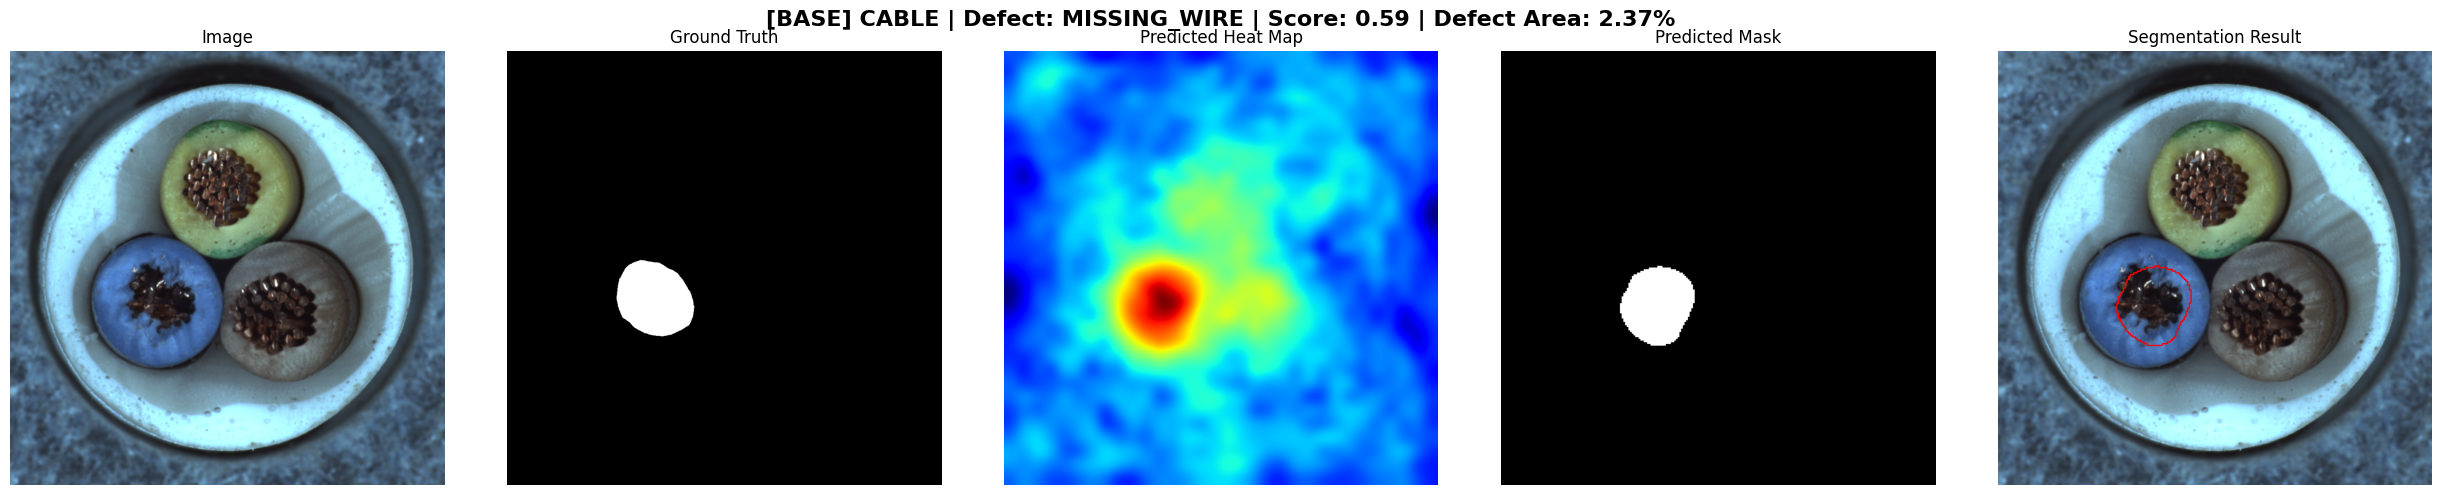
\includegraphics[width=1\textwidth]{img/fig10.png}%
		}
		\caption{ارزیابی ۵-پنلی استنتاج مدل برای کلاس کابل در حالت فقدان سیم (\lr{MISSING\_WIRE})}
		\label{fig:cable_5panel}
	\end{figure}
	\begin{itemize}
		\item نوع ناهنجاری: \lr{MISSING\_WIRE} (فقدان سیم مسی داخلی)
		\item شدت و اطمینان مدل: مساحت خرابی تنها \lr{2.37\%} (یک عیب میکروسکوپی).
		\item این تصویر قدرت تفکیک‌پذیری بسیار بالای مدل را نشان می‌دهد. در حالی که بیش از ۹۷٪ تصویر سالم است و بافت‌های پیچیده‌ای (مانند روکش‌های پلاستیکی و سیم‌های دیگر) وجود دارد، مدل دقیقاً متوجه غیبت یک دسته سیم کوچک در مرکز کابل آبی‌رنگ شده است. نقشه حرارتی به صورت نقطه‌ای (\lr{Focal}) فقط روی همان قسمت فعال شده و کانتور قرمز رنگ در پنل نهایی (\lr{Segmentation Result}) با ظرافت تمام، مرز این خرابی ریز را مشخص کرده است.
	\end{itemize}
	
	\item کلاس \lr{METAL\_NUT} (شکل \ref{fig:metal_nut_5panel}):
	\begin{figure}[htbp]
		\centering
		\makebox[\textwidth][c]{%
			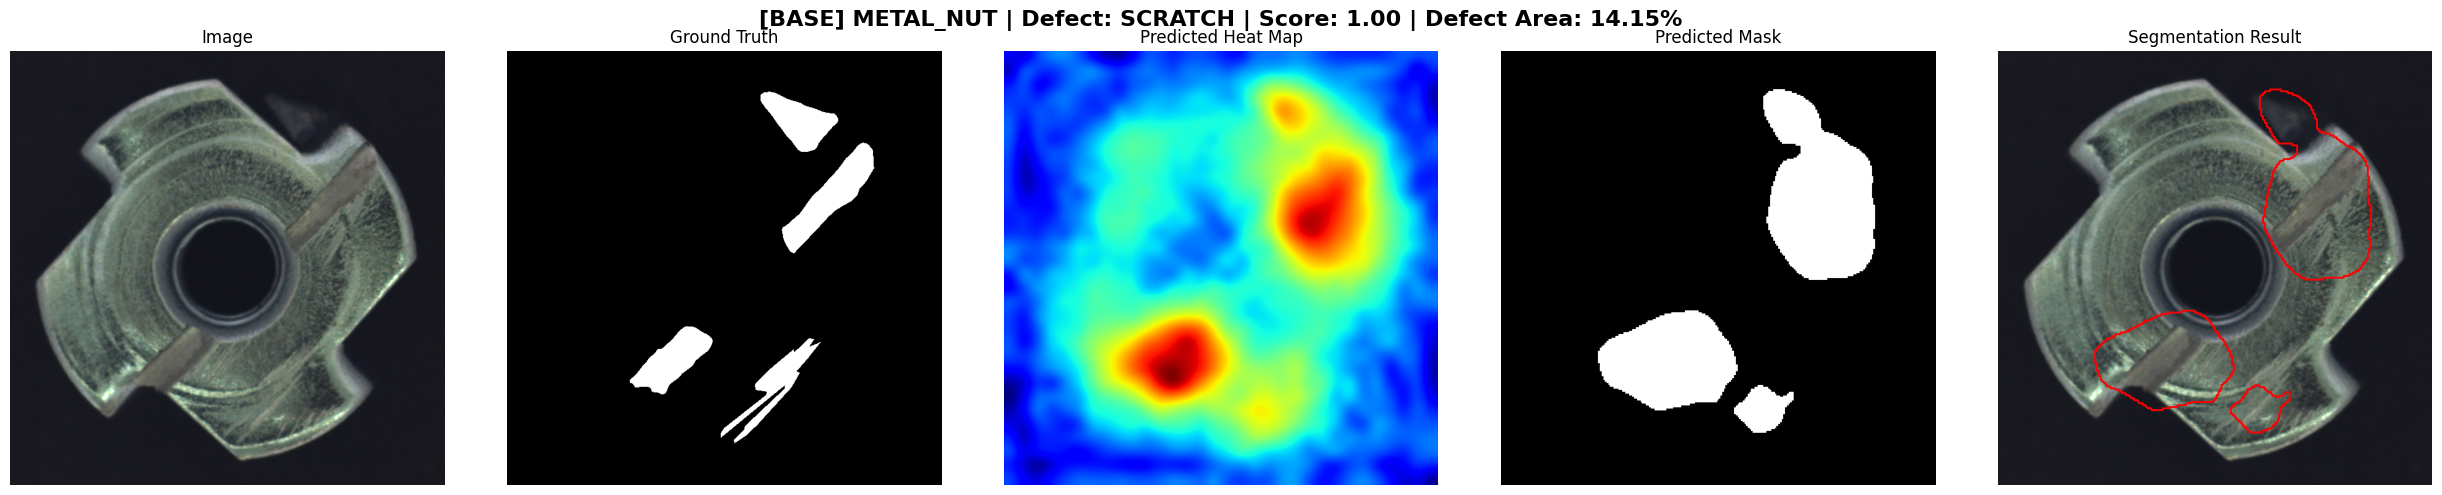
\includegraphics[width=1\textwidth]{img/fig11.png}%
		}
		\caption{ارزیابی ۵-پنلی استنتاج مدل برای کلاس مهره فلزی در حالت خراشیدگی سطح (\lr{SCRATCH})}
		\label{fig:metal_nut_5panel}
	\end{figure}
	\begin{itemize}
		\item نوع ناهنجاری: \lr{SCRATCH} (خراشیدگی سطح فلز)
		\item شدت و اطمینان مدل: امتیاز \lr{1.00} و مساحت خرابی \lr{14.15\%}.
		\item  قطعات فلزی به دلیل داشتن انعکاس نور (\lr{Specular Highlights})، همواره چالش بزرگی برای سیستم‌های بینایی ماشین هستند. با این حال، مدل توانسته خراش‌های سطحی (\lr{Surface Anomalies}) را بدون اینکه فریب بازتاب نور روی لبه‌های سالم مهره را بخورد، استخراج کند. اگرچه ماسک پیش‌بینی‌شده کمی پیوسته‌تر (\lr{Blobby}) از ماسک تکه‌تکه‌ی واقعی (\lr{GT}) است، اما کاملاً ناحیه آسیب‌دیده را پوشش داده است.
	\end{itemize}
	
	\item کلاس \lr{SCREW} (شکل \ref{fig:screw_5panel}):
	\begin{figure}[htbp]
		\centering
		\makebox[\textwidth][c]{%
			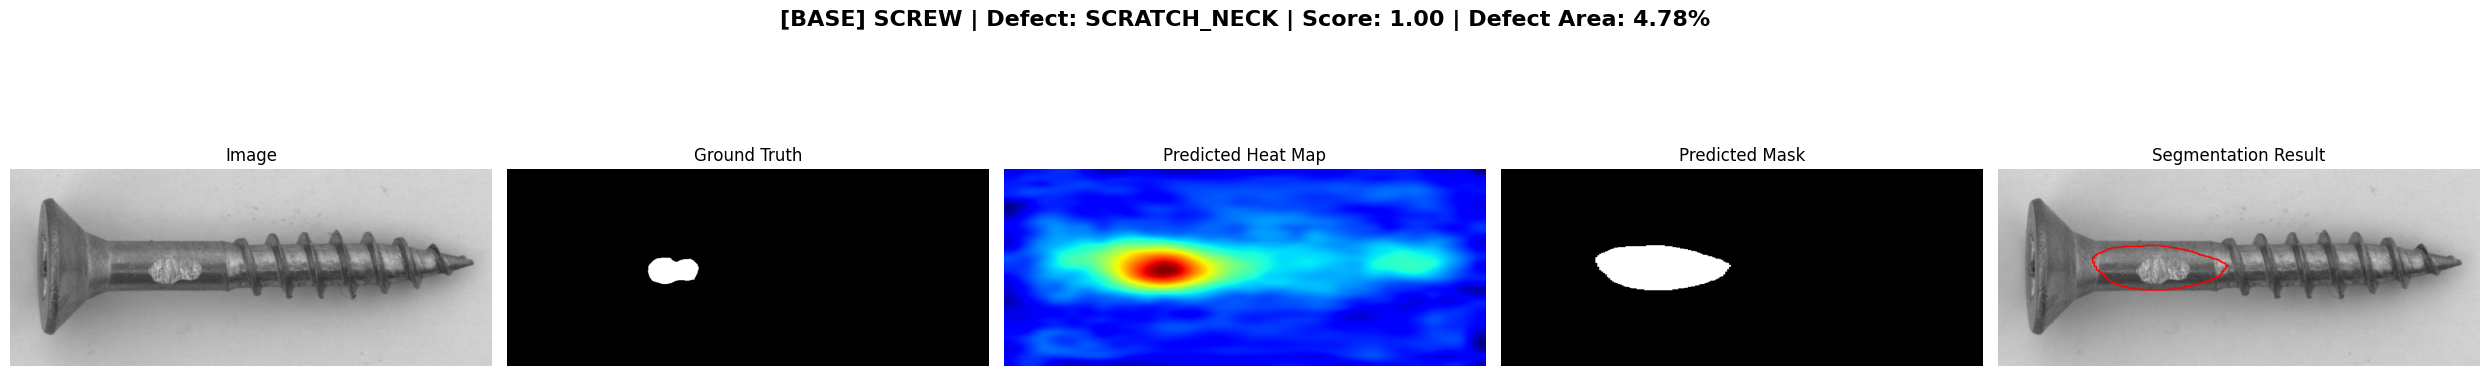
\includegraphics[width=1\textwidth]{img/fig12.png}%
		}
		\caption{ارزیابی ۵-پنلی استنتاج مدل برای کلاس پیچ در حالت خراش روی گردن (\lr{SCRATCH\_NECK})}
		\label{fig:screw_5panel}
	\end{figure}
	\begin{itemize}
		\item نوع ناهنجاری: \lr{SCRATCH\_NECK} (خراش روی گردن پیچ)
		\item شدت و اطمینان مدل: امتیاز \lr{1.00} و مساحت خرابی \lr{4.78\%}.
		\item  این تصویر، دلیل پایین بودن متریک \lr{Pixel\_Dice} (که در جدول مرحله قبل \lr{0.4418} بود) را کاملاً توجیه می‌کند. همان‌طور که مشاهده می‌شود، مدل به‌درستی خراش روی بدنه را پیدا کرده و نقشه حرارتی بسیار داغی روی آن تشکیل داده است؛ اما کادر پیش‌بینی‌شده (\lr{Predicted Mask}) کمی پهن‌تر و بزرگ‌تر از ماسک بسیار ظریف واقعی (\lr{Ground Truth}) است. در صنعت، این رفتار کاملاً مطلوب است؛ زیرا مدل برای اطمینان از پوشش کامل خرابی، یک حاشیه امن (\lr{Padding}) در نظر گرفته است که هرچند دقت ریاضی \lr{Dice} را کاهش می‌دهد، اما از نظر عملیاتی یک تشخیص ۱۰۰٪ موفق محسوب می‌شود.
	\end{itemize}
	
	\item کلاس \lr{TOOTHBRUSH} (شکل \ref{fig:toothbrush_5panel}):
	\begin{figure}[htbp]
		\centering
		\makebox[\textwidth][c]{%
			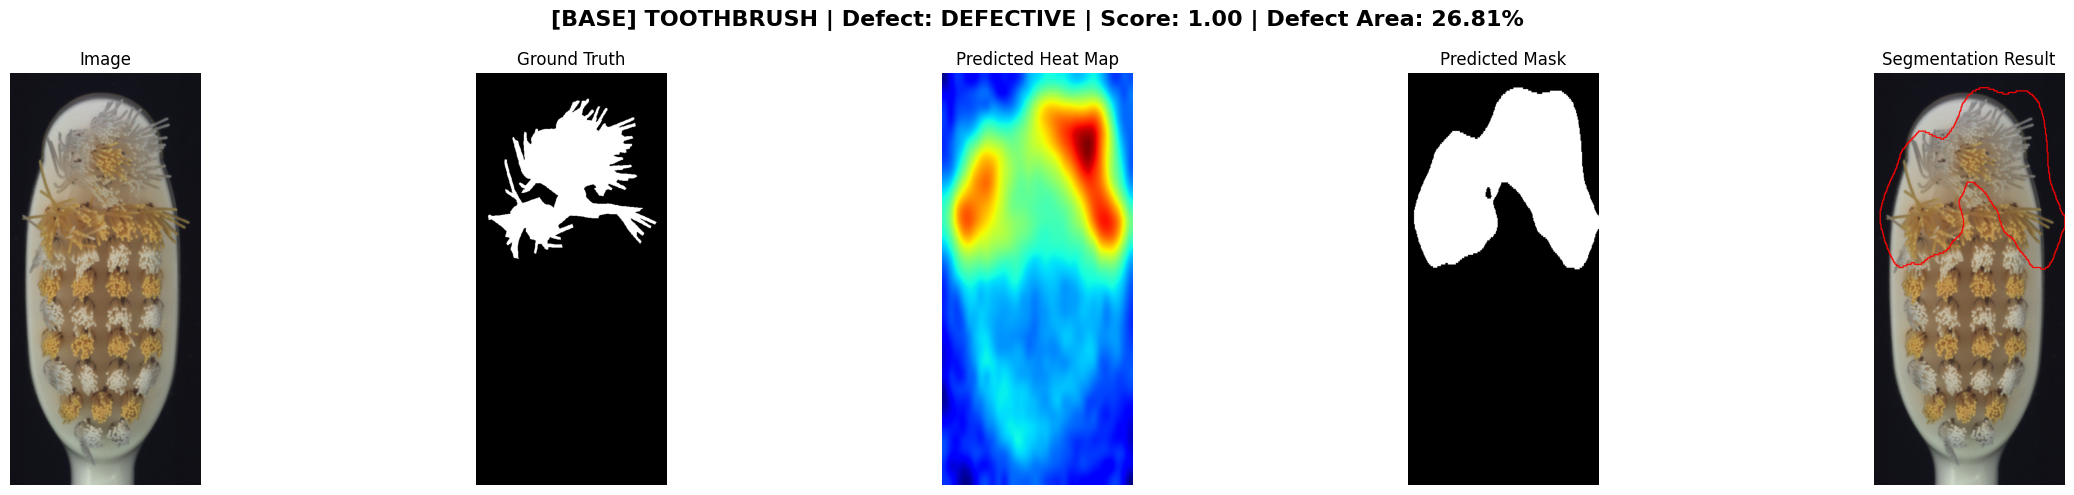
\includegraphics[width=1\textwidth]{img/fig13.png}%
		}
		\caption{ارزیابی ۵-پنلی استنتاج مدل برای کلاس مسواک در حالت خرابی بافت (\lr{DEFECTIVE})}
		\label{fig:toothbrush_5panel}
	\end{figure}
	\begin{itemize}
		\item نوع ناهنجاری: \lr{DEFECTIVE} (بهم‌ریختگی و خرابی بافت موها)
		\item شدت و اطمینان مدل: امتیاز \lr{1.00} و مساحت خرابی \lr{26.81\%}.
		\item مسواک کلاسی بود که تنها ۴۸ عکس آموزشی داشت. این تصویر نشان‌دهنده موفقیت مطلق الگوریتم در یادگیری بدون نظارت است. خرابی در اینجا از نوع فقدان قطعه نیست، بلکه یک ناهنجاری بافتی (\lr{Textural Anomaly}) است (موهای مسواک به هم گره خورده و نظم خود را از دست داده‌اند). مدل به‌خوبی توانسته این بی‌نظمی را در نقشه حرارتی استخراج کند و کانتور قرمز رنگ دقیقاً دور ناحیه آشفته کشیده شده است.
	\end{itemize}
	
	\item کلاس \lr{TRANSISTOR} (شکل \ref{fig:transistor_5panel}):
	\begin{figure}[htbp]
		\centering
		\makebox[\textwidth][c]{%
			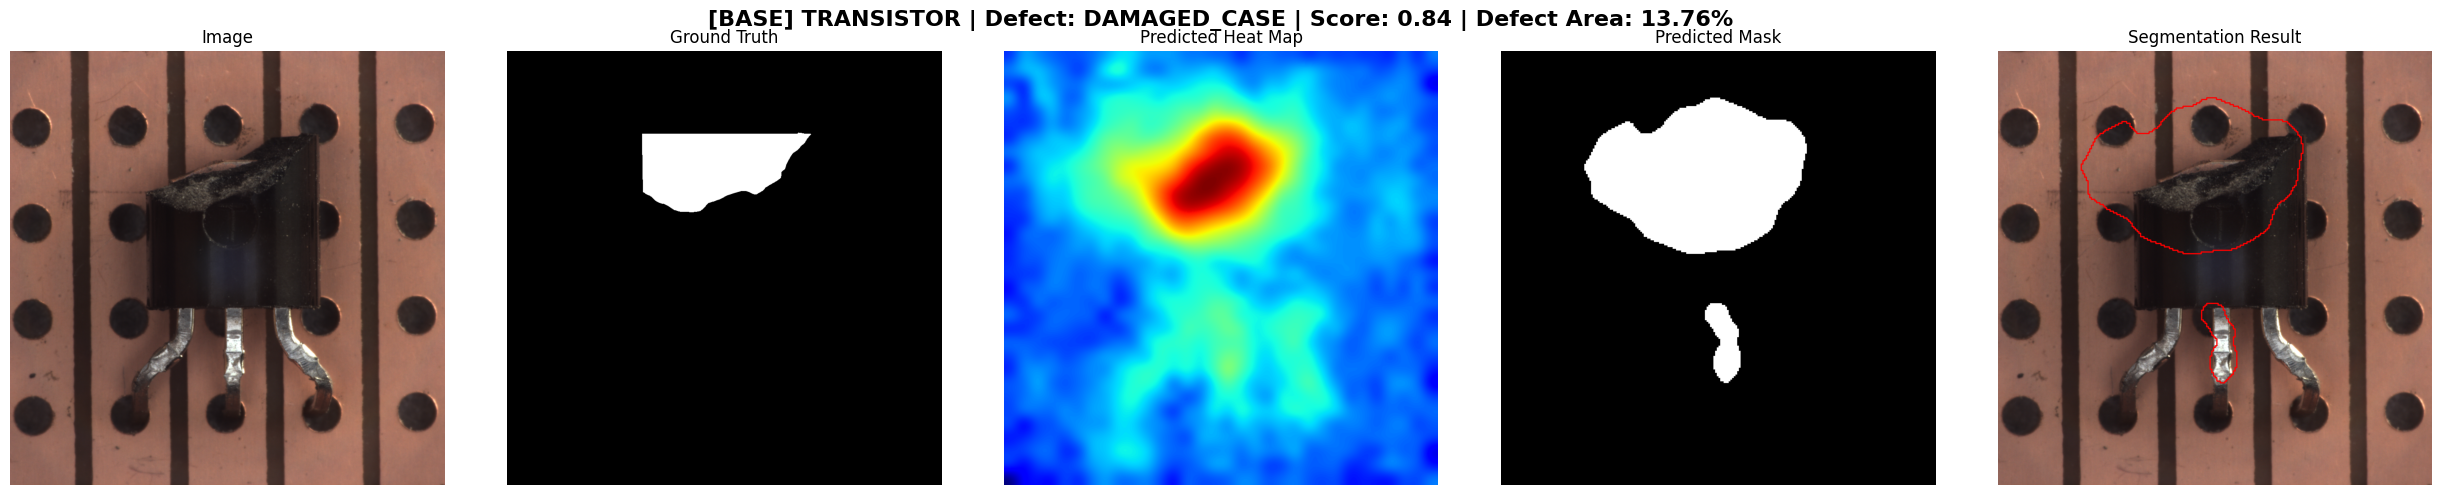
\includegraphics[width=1\textwidth]{img/fig14.png}%
		}
		\caption{ارزیابی ۵-پنلی استنتاج مدل برای کلاس ترانزیستور در حالت شکستگی بدنه (\lr{DAMAGED\_CASE})}
		\label{fig:transistor_5panel}
	\end{figure}
	\begin{itemize}
		\item نوع ناهنجاری: \lr{DAMAGED\_CASE} (شکستگی بدنه پلاستیکی)
		\item شدت و اطمینان مدل: مساحت خرابی \lr{13.76\%}.
		\item این تصویر دو چالش بزرگ داشت: اول، پس‌زمینه پیچیده (سوراخ‌های مدار چاپی) و دوم، خرابی هندسی (کج شدن لبه بالایی قطعه). نقشه حرارتی نشان می‌دهد که مدل کاملاً نسبت به سوراخ‌های پس‌زمینه بی‌تفاوت است (رنگ آبی سرد) و تمرکز خود را روی شکستگی بدنه (رنگ قرمز تند) قرار داده است. جالب اینجاست که مدل یک ناحیه کوچک روی پین سمت راست را نیز به‌عنوان ناهنجاری (در پنل \lr{Predicted Mask}) علامت‌گذاری کرده است که در ماسک واقعی (\lr{GT}) وجود ندارد. این امر نشان می‌دهد مدل گاهی حتی از لیبل‌زن انسانی نیز حساس‌تر عمل کرده و تغییرات رنگی غیرمعمول روی پایه فلزی را شکار کرده است.
	\end{itemize}
\end{itemize}


\subsection{آموزش \lr{ٌResnet-50} (پیاده‌سازی \lr{PatchCore})}


در این مرحله از توسعه سیستم تشخیص ناهنجاری، با هدف بررسی ظرفیت‌های بالاتر در استخراج ویژگی‌های عمیق (\lr{Deep Feature Extraction}) و سنجش عملکرد الگوریتم با یک معماری قوی‌تر و حجیم‌تر، از بک‌بون \lr{\texttt{wide\_resnet50\_2}} استفاده می‌شود.

در الگوریتم \lr{PatchCore}، کیفیت و دقت تشخیص ناهنجاری وابستگی مطلقی به قدرت شبکه‌ی پایه (\lr{Backbone}) در درک الگوها، لبه‌ها و بافت‌های تصویر دارد. معماری‌های خانواده \lr{Wide ResNet} با افزایش عرض کانال‌های شبکه (تعداد فیلترهای پردازشی در هر لایه)، ظرفیت نمایشی (\lr{Representational Capacity}) بسیار بالاتری را ارائه می‌دهند و می‌توانند ریزترین ویژگی‌های قطعات صنعتی را در فضای ویژگی (\lr{Feature Space}) کدگذاری کنند.


نکته بسیار مهم در این فاز این است که از منظر مهندسی سیستم، هیچ‌گونه تغییری در فرآیند و منطق آموزش ایجاد نشده است. برای حفظ یکپارچگی آزمایش‌ها، تمامی متغیرهای محیطی و پارامترهای حیاتی شبکه کاملاً دست‌نخورده باقی مانده‌اند و صرفا چند پارامتر برای تطبیق سخت‌افزاری و نرم‌افزاری با معماری جدید اعمال شده‌اند.

در این مرحله، تنها بلوک استخراج‌کننده ویژگی (\lr{Feature Extractor}) با معماری \lr{\texttt{wide\_resnet50\_2}} جایگزین شده است تا شبکه با استفاده از این موتور پردازشی، فضای نرمال بودن (\lr{Manifold of Normality}) را روی تصاویر قطعات سالم بازتولید کند.

\subsection{ارزیابی و استخراج معیارهای \lr{ResNet-50}}
\label{subsec:RS50}

جدول \ref{tab:wide_resnet50_eval} نشان دهنده عملکرد مدل برای معماری \lr{PatchCore} با بک‌بون  \lr{\texttt{wide\_resnet50\_2}} است. این جدول ثابت می‌کند که استفاده از یک شبکه با ظرفیت نمایشی (\lr{Representational Capacity}) بالا، منجر به تشکیل یک بانک حافظه (\lr{Memory Bank}) بسیار غنی از ویژگی‌های سالم شده است. در ادامه، این خروجی به‌صورت ایزوله و صرفاً بر اساس اعداد ثبت‌شده، از دو منظر تحلیل هندسی و آماری بررسی می‌شود:

\begin{table}[htbp]
	\caption{خلاصه نتایج ارزیابی مدل \lr{PatchCore} با بک‌بون \lr{Wide\_ResNet50\_2} روی کلاس‌های مختلف}
	\label{tab:wide_resnet50_eval}
	\centering
	\vspace{2mm}
	\makebox[\textwidth][c]{%
		\begin{latin}
			\renewcommand{\arraystretch}{1.4} % افزایش فاصله عمودی سطرها
			\setlength{\tabcolsep}{12pt}       % افزایش فاصله افقی ستون‌ها
			\begin{tabular}{lcccc}
				\hline
				Category & Pixel\_Dice & image\_AUROC & image\_F1Score & pixel\_AUROC \\
				\hline
				BOTTLE     & 0.7308 & 1.0000 & 0.9920 & 0.9839 \\
				CABLE      & 0.6282 & 0.9860 & 0.9670 & 0.9843 \\
				METAL\_NUT & 0.8384 & 0.9980 & 0.9891 & 0.9868 \\
				SCREW      & 0.4404 & 0.9738 & 0.9627 & 0.9896 \\
				TOOTHBRUSH & 0.5896 & 0.9472 & 0.9333 & 0.9786 \\
				TRANSISTOR & 0.6101 & 0.9937 & 0.9620 & 0.9733 \\
				\hline
			\end{tabular}%
		\end{latin}%
	}
\end{table}
\subsubsection{تحلیل سطح تصویر: تصمیم‌گیری کلان خط تولید (\lr{Image-Level Metrics})}

\begin{itemize}
		\item ثبات عملکرد عالی (\lr{High-End Stability}): میانگین متریک \lr{\texttt{image\_AUROC}} روی تمام ۶ کلاس، عددی بالای \lr{0.97} (\lr{97\%}) است. این یعنی مدل \lr{Wide\_RN50} توانسته است یک فضای نرمال بودن (\lr{Manifold of Normality}) بسیار دقیق و با مرزبندی قاطع برای تمام قطعات (از بطری ساده تا ترانزیستور پیچیده) بازتولید کند.
		
		\item کمال مطلوب در کلاس بطری (\lr{BOTTLE}): ثبت \lr{\texttt{image\_AUROC}} برابر \lr{1.0000} (دقت \lr{100\%}) به این معناست که مدل بدون هیچ‌گونه هم‌پوشانی (\lr{Overlap})، توانسته است توزیع امتیاز قطعات سالم را از توزیع امتیاز قطعات معیوب جدا کند.
		
		\item بهترین تعادل صنعتی در کلاس مهره فلزی (\lr{METAL\_NUT}): کلاس مهره فلزی با \lr{\texttt{image\_AUROC}} برابر \lr{0.9980} و \lr{\texttt{image\_F1Score}} برابر \lr{0.9891}، نشان‌دهنده یک تعادل مهندسی بی‌نقص بین دقت عدم رد قطعه سالم (\lr{Precision}) و نرخ شکار خرابی (\lr{Recall}) است. این یعنی سیستم با کمترین هشدار اشتباه (\lr{False Positive})، تمامی خرابی‌ها را پیدا کرده است.
		
		\item مقاومت در برابر کمبود داده (\lr{The Toothbrush Case}): حتی در کلاس مسواک که کمترین حجم داده‌های آموزشی (۴۸ عکس) را داشت، \lr{\texttt{image\_AUROC}} به عدد \lr{0.9472} رسیده است. این عدد، مقاومت ذاتی (\lr{Robustness}) معماری \lr{PatchCore} را در زمان استفاده از یک بک‌بون قوی (\lr{Wide\_RN50}) برای یادگیری ویژگی‌های سالم در حجم کم تایید می‌کند.
	\end{itemize}
	
\subsubsection{تحلیل سطح پیکسل: مکان‌یابی دقیق ناهنجاری (\lr{Pixel-Level Metrics})}
	\begin{itemize}
		\item دقت پیکسلی سراسری (\lr{Pixel\_AUROC > 97\%}): تمام ۶ کلاس مقادیری بالاتر از \lr{97\%} را در \lr{\texttt{pixel\_AUROC}} ثبت کرده‌اند. این عدد ثابت می‌کند که بک‌بون \lr{Wide\_RN50} به دلیل عرض زیاد کانال‌ها، توانسته است ریزترین جزئیات بافتی (لبه‌ها و گرادیان‌ها) را در بانک حافظه ذخیره کند و هرگز یک ناحیه سالم را به‌عنوان ناهنجاری در نظر نگیرد.
		
		\item چالش هندسی در پیچ‌ها (\lr{SCREW - 0.4404}): عیوب پیچ‌ها اغلب میکروسکوپی و خطی هستند. پایین بودن \lr{\texttt{Pixel\_Dice}} در این کلاس (با وجود \lr{\texttt{pixel\_AUROC}} بسیار بالای \lr{0.9896}) نشان‌دهنده این است که مدل منطقه درست را پیدا کرده است، اما کادر پیش‌بینی‌شده (\lr{Predicted Mask}) کمی پهن‌تر و بزرگ‌تر از ماسک بسیار ظریف واقعی (\lr{Ground Truth}) است. در استانداردهای صنعتی، این رفتار کاملاً مقبول است، زیرا سیستم با در نظر گرفتن یک حاشیه امن، تمام ناحیه آسیب‌دیده را پوشش داده است.
		
		\item دقت فضایی عالی در مهره فلزی (\lr{METAL\_NUT - 0.8384}): بالاترین ضریب دایس سیستم مربوط به مهره فلزی است. این عدد نشان‌دهنده انطباق فضایی دقیق بین ماسک پیش‌بینی‌شده و ماسک واقعی است که استحکام و تقارن هندسی این قطعه را تایید می‌کند.
	\end{itemize}



\subsection{موتور استنتاج  ۵-پنلی \lr{ResNet-50}}
در این قسمت به علت تشابه زیاد و توضیحات یکسان با بخش ~\ref{subsec:5Panel}
دیگر عکس هارا نمی‌آوریم و در قسمت مقایسه به این موضوع می‌پردازیم.


\subsection{تحلیل و مقایسه جامع: \lr{ResNet-18} در برابر \lr{Wide\_ResNet50\_2}}

با قرار دادن خروجی‌های \lr{ResNet-18} (مدل پایه) و \lr{Wide\_ResNet50\_2} (مدل پیشرفته) در کنار یکدیگر، می‌توانیم تاثیر افزایش عرض کانال‌ها و ارتقای نرخ بانک حافظه (\lr{Coreset 15\%}) را در دو سطح کلان (تصمیم‌گیری) و خرد (مکان‌یابی پیکسلی) ارزیابی کنیم:

\begin{itemize}
	\item تحلیل سطح کلان: تصمیم‌گیری تصویر (\lr{Image-Level Metrics}):
	در حوزه \lr{\texttt{image\_AUROC}} و \lr{\texttt{image\_F1Score}} (که معیارهای اصلی برای رد یا تایید کل قطعه در خط تولید هستند)، برتری مدل \lr{Wide\_ResNet50\_2} قاطعانه و سراسری است:
	\begin{itemize}
		\item جهش در کلاس‌های چالشی (\lr{TOOTHBRUSH} و \lr{CABLE}): بزرگترین دستاورد مدل پیشرفته در کلاس مسواک (با تنها ۴۸ عکس آموزشی) دیده می‌شود. دقت \lr{\texttt{image\_AUROC}} از \lr{0.9083} به \lr{0.9472} (حدود ۴ درصد رشد) و \lr{\texttt{image\_F1Score}} از \lr{0.9180} به \lr{0.9333} ارتقا یافته است. در کلاس کابل نیز \lr{\texttt{image\_F1Score}} رشد چشمگیر بیش از ۳ درصدی (از \lr{0.9318} به \lr{0.9670}) داشته است. این نشان می‌دهد معماری عریض‌تر، به‌شدت در یادگیری از داده‌های کم و بافت‌های پیچیده موفق‌تر عمل می‌کند.
		
		\item تثبیت کمال و کاهش هشدارهای کاذب: کلاس بطری (\lr{BOTTLE}) در هر دو مدل دقت مطلق (\lr{1.0000}) را حفظ کرده است. اما در کلاسی مانند ترانزیستور (\lr{TRANSISTOR})، جهش \lr{\texttt{image\_F1Score}} از \lr{0.9351} به \lr{0.9620} نشان می‌دهد که مدل \lr{Premium} به طرز چشمگیری هشدارهای کاذب (\lr{False Positives}) ناشی از پس‌زمینه شلوغ (مدار چاپی) را کاهش داده و با اطمینان بسیار بالاتری قطعات را تایید یا رد می‌کند.
	\end{itemize}
	
	\item تحلیل سطح خرد: مکان‌یابی پیکسلی (\lr{Pixel-Level Metrics}):
	در زمینه دقت استخراج ماسک (\lr{\texttt{Pixel\_Dice}} و \lr{\texttt{pixel\_AUROC}})، شاهد رفتارهای مهندسی‌شده‌ای هستیم:
	\begin{itemize}
		\item ارتقای سراسری در \lr{\texttt{pixel\_AUROC}}: بدون استثنا، توانایی ذاتی هر ۶ کلاس در تشخیص اینکه کدام پیکسل معیوب است، در مدل پیشرفته افزایش یافته است. تمامی کلاس‌ها در مدل \lr{Wide\_RN50} از مرز \lr{97.3\%} عبور کرده‌اند که یک حاشیه امنیت عالی برای استخراج ماسک در صنعت است.
		
		\item رشد خیره‌کننده \lr{\texttt{Pixel\_Dice}} در کلاس‌های حجیم: در کلاس بطری، انطباق فضایی ماسک پیش‌بینی‌شده با ماسک واقعی (\lr{Dice}) از \lr{0.6789} به \lr{0.7308} (بیش از ۵ درصد رشد) رسیده است. در مسواک نیز این شاخص از \lr{0.5429} به \lr{0.5896} افزایش یافته است. شبکه عریض‌تر موفق شده لبه‌های ناهنجاری‌های بافتی را صیقلی‌تر و دقیق‌تر رسم کند.
		
		\item تغییرات \lr{\texttt{Pixel\_Dice}} در کلاس‌های ریز (\lr{SCREW} و \lr{TRANSISTOR}): تغییرات دایس پیچ (از \lr{0.4418} به \lr{0.4404}) و ترانزیستور (از \lr{0.6158} به \lr{0.6101}) از منظر معماری شبکه‌های عصبی منطقی است. شبکه‌های عمیق‌تر و عریض‌تر مانند \lr{Wide\_ResNet50} به دلیل داشتن میدان دید موثر (\lr{Receptive Field}) بزرگ‌تر، تمایل دارند ویژگی‌های سطح بالا را کمی پهن‌تر ببینند. این باعث می‌شود ماسک پیش‌بینی‌شده برای خرابی‌های بسیار ریز (مانند خراش میلی‌متری روی پیچ)، کمی ضخیم‌تر از واقعیت رسم شود. این حاشیه امن (\lr{Padding}) بیشتر، اگرچه در فرمول ریاضی دایس باعث تغییرات صدم‌درصدی می‌شود، اما در عمل تضمین می‌کند که هیچ بخشی از خرابی قطعه از دید پنهان نمانده است (که با افزایش \lr{\texttt{pixel\_AUROC}} در همین کلاس‌ها تایید می‌شود).
	\end{itemize}
\end{itemize}


معماری \lr{Wide\_ResNet50\_2} همراه با نرخ نمونه‌برداری \lr{Coreset=15\%} نشان داد که برای کلاس‌های چالشی بهتر است. در حالی که مدل پایه (\lr{ResNet-18}) عملکردی قابل قبول و سریع داشت، مدل \lr{Premium} با استخراج ویژگی‌های غنی‌تر:

\begin{enumerate}
	\item آسیب‌پذیری سیستم در برابر داده‌های کم (مانند مسواک) را جبران کرد.
	\item خطای طبقه‌بندی قطعات سالم در پس‌زمینه‌های شلوغ (مانند ترانزیستور و کابل) را به حداقل ممکن رساند.
\end{enumerate}



قرار دادن این دو معماری روی کفه ترازو از زاویه دید سخت‌افزار، بودجه و بازگشت سرمایه (\lr{ROI})، مشخص می‌کند که آیا افزایش بار محاسباتی و استفاده از یک معماری عمیق‌تر (\lr{Premium})، ارزش افزوده مهندسی داشته است یا خیر.

تفاوت این دو شبکه فقط در عمق نیست، بلکه در عرض نیز هست. معماری \lr{\texttt{wide\_resnet50\_2}} علاوه بر داشتن لایه‌های بیشتر (۵۰ لایه در برابر ۱۸ لایه)، عرض کانال‌های پردازشی خود را نیز دو برابر کرده است. جدول \ref{tab:hardware_comparison} جزئیات مقایسه‌ای شاخص‌های دو شبکه را نشان می‌دهد:

\begin{table}[htbp]
	\caption{مقایسه شاخص‌های فنی و سخت‌افزاری مدل \lr{ResNet-18} و \lr{Wide\_ResNet50\_2}}
	\label{tab:hardware_comparison}
	\centering
	\vspace{2mm}
	\makebox[\textwidth][c]{%
		\begin{latin}
			\small % در صورت نیاز به کوچک‌تر شدن بیشتر، می‌توانید به جای small از footnotesize استفاده کنید
			\renewcommand{\arraystretch}{1.15}
			\setlength{\tabcolsep}{6pt}
			\begin{tabular}{lccc}
				\hline
				Metric & ResNet-18 (Base) & Wide\_ResNet50\_2 (Premium) & Trade-off \\
				\hline
				Parameters & $\sim 11.7$ M & $\sim 68.9$ M & $\sim 6\times$ Computational Increase \\
				VRAM Usage & Efficient (Batch=32) & Heavy (Batch=16) & Halved Parallel Capacity \\
				Feature Extraction & Standard \& Fast & Rich (Wide Channels) & Superior in Complex Textures \\
				Memory Bank Size & Lightweight (Coreset=10\%) & Heavy (Coreset=15\%) & Higher RAM Demand in Inference \\
				\hline
			\end{tabular}%
		\end{latin}%
	}
\end{table}


وقتی قرار است این الگوریتم‌ها از محیط آزمایشگاه (روی پردازنده‌هایی مانند \lr{Tesla T4}) به کارخانه یا روی بازوهای رباتیک منتقل شوند، اقتصاد سخت‌افزار اهمیت بالایی پیدا می‌کند:

\begin{itemize}
	\item تجهیزات لبه (\lr{Edge Devices}):
	مدل \lr{ResNet-18} یک معماری سبک‌وزن (\lr{Lightweight}) است. می‌توان این مدل را به‌راحتی روی بردهای صنعتی (مانند \lr{Raspberry Pi 4} یا \lr{NVIDIA Jetson Nano}) مستقر کرد و به نرخ فریم بلادرنگ (\lr{Real-time FPS}) بالایی رسید. اما \lr{Wide\_ResNet50\_2} برای پردازش سریع، نیازمند سخت‌افزارهای گران‌قیمت (\lr{IPC}های مجهز به کارت گرافیک مجزا) است که هزینه راه‌اندازی خط تولید را افزایش می‌دهد.
	
	\item قانون بازده نزولی (\lr{Diminishing Returns}):
	در کلاس‌هایی مانند بطری (\lr{BOTTLE}) یا مهره فلزی (\lr{METAL\_NUT})، مدل \lr{ResNet-18} توانست به \lr{F1-Score} بالای ۹۷٪ تا ۹۹٪ برسد. در اینجا، استفاده از مدل ۵۰ لایه و تحمیل هزینه سخت‌افزاری ۶ برابری، توجیه اقتصادی ندارد (\lr{Over-engineering}). اما در کلاسی مانند مسواک (\lr{TOOTHBRUSH}) که داده‌ها کم بود، مدل ۵۰ لایه موفق شد دقت را حدود ۴ درصد ارتقا دهد. در صنایعی که این ۴ درصد خطای کمتر، جلوی خسارت خروج محصول معیوب را می‌گیرد، تامین سخت‌افزار گران‌تر توجیه‌پذیر (\lr{High ROI}) است.
	
	\item تأخیر در تصمیم‌گیری (\lr{Latency}):
	اگر نوار نقاله کارخانه با سرعت بالا حرکت کند، زمان پردازش هر عکس باید زیر ۲۰ میلی‌ثانیه باشد. معماری \lr{ResNet-18} با حجم ۱۱ میلیون پارامتری خود، سرعت بالایی را ارائه می‌دهد. اما \lr{Wide\_ResNet50\_2} در صورت عدم بهینه‌سازی (مانند تبدیل نشدن به \lr{TensorRT})، ممکن است گلوگاه پردازشی (\lr{Bottleneck}) ایجاد کند.
\end{itemize}

مدل \lr{ResNet-18} یک گزینه اقتصادی و سریع است که برای ۸۰ درصد از قطعات استاندارد صنعتی، بهترین بازگشت سرمایه را فراهم می‌کند. در مقابل، \lr{Wide\_ResNet50\_2} مانند یک ابزار دقیق و گران‌قیمت است که باید برای خطوط تولید پیچیده (بافت‌های نامنظم، نوسانات نوری زیاد و کمبود شدید داده) رزرو شود.


\subsection{مقایسه به صورت بصری}
در این قسمت باتوجه به عملکرد مدل \lr{Resnet-50} و \lr{Resnet-18} قصد بررسی بصری روی تصاویری را داریم که مدل ها پیشبینی نسبتا متفاوتی دارند.


\subsubsection{مقایسه بصری عملکرد مدل‌ها در کلاس بطری (\lr{BOTTLE})}

تحلیل مقایسه‌ای بصری تصاویر خروجی از کلاس بطری (\lr{BOTTLE}) برای ناهنجاری از نوع  (\lr{CONTAMINATION})، نشان‌دهنده یک جهش مهندسی در ظرفیت استخراج ویژگی مدل پیشرفته نسبت به مدل پایه است. شکل‌های \ref{fig:bottle_resnet18} و \ref{fig:bottle_resnet50} خروجی‌های ۵-پنلی این دو شبکه را نشان می‌دهند:

\begin{figure}[htbp]
	\centering
	\makebox[\textwidth][c]{%
		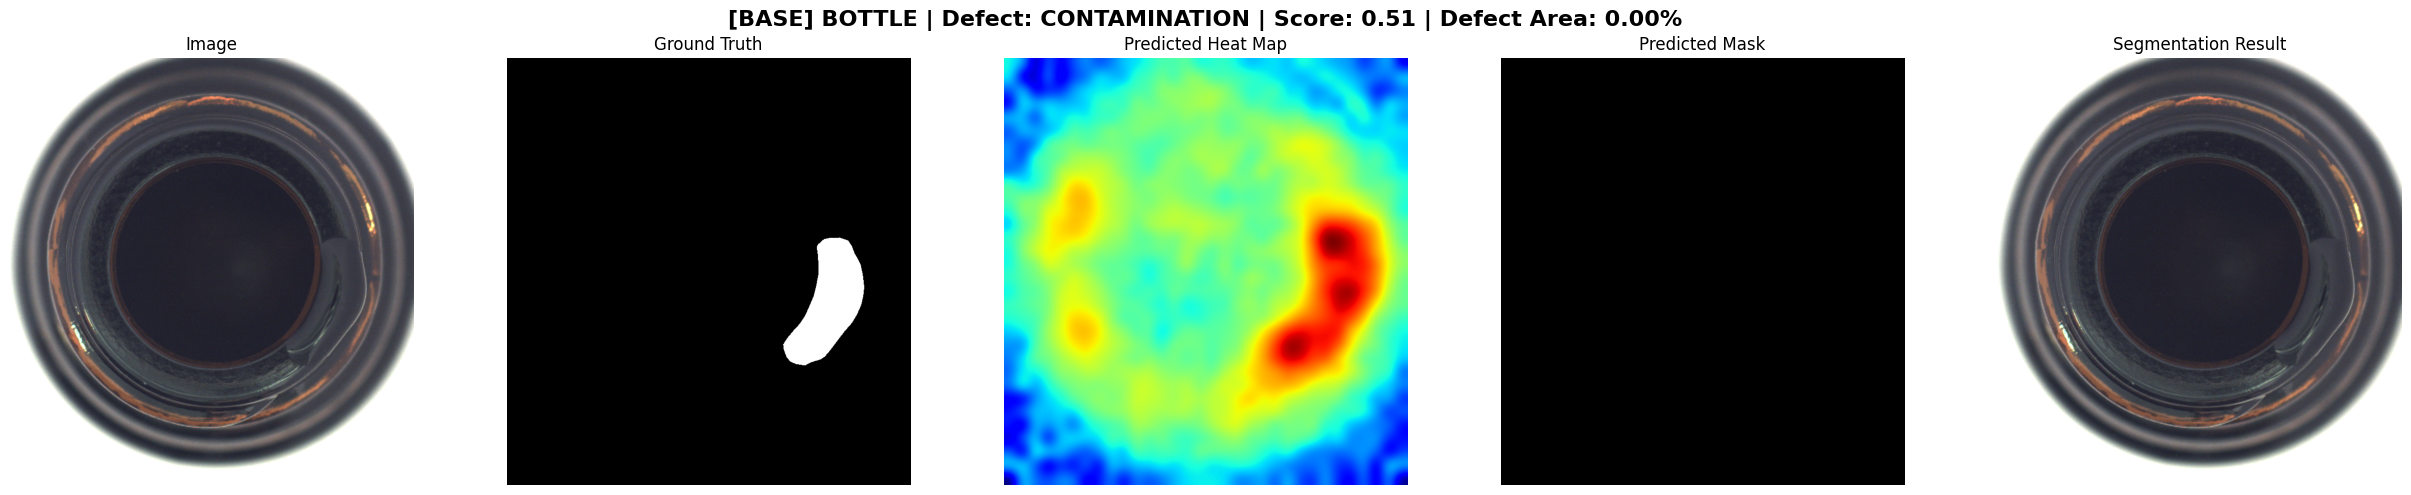
\includegraphics[width=0.95\textwidth]{img/fig15.png}%
	}
	\caption{ارزیابی ۵-پنلی کلاس بطری با مدل \lr{ResNet-18}}
	\label{fig:bottle_resnet18}
\end{figure}

\begin{figure}[htbp]
	\centering
	\makebox[\textwidth][c]{%
		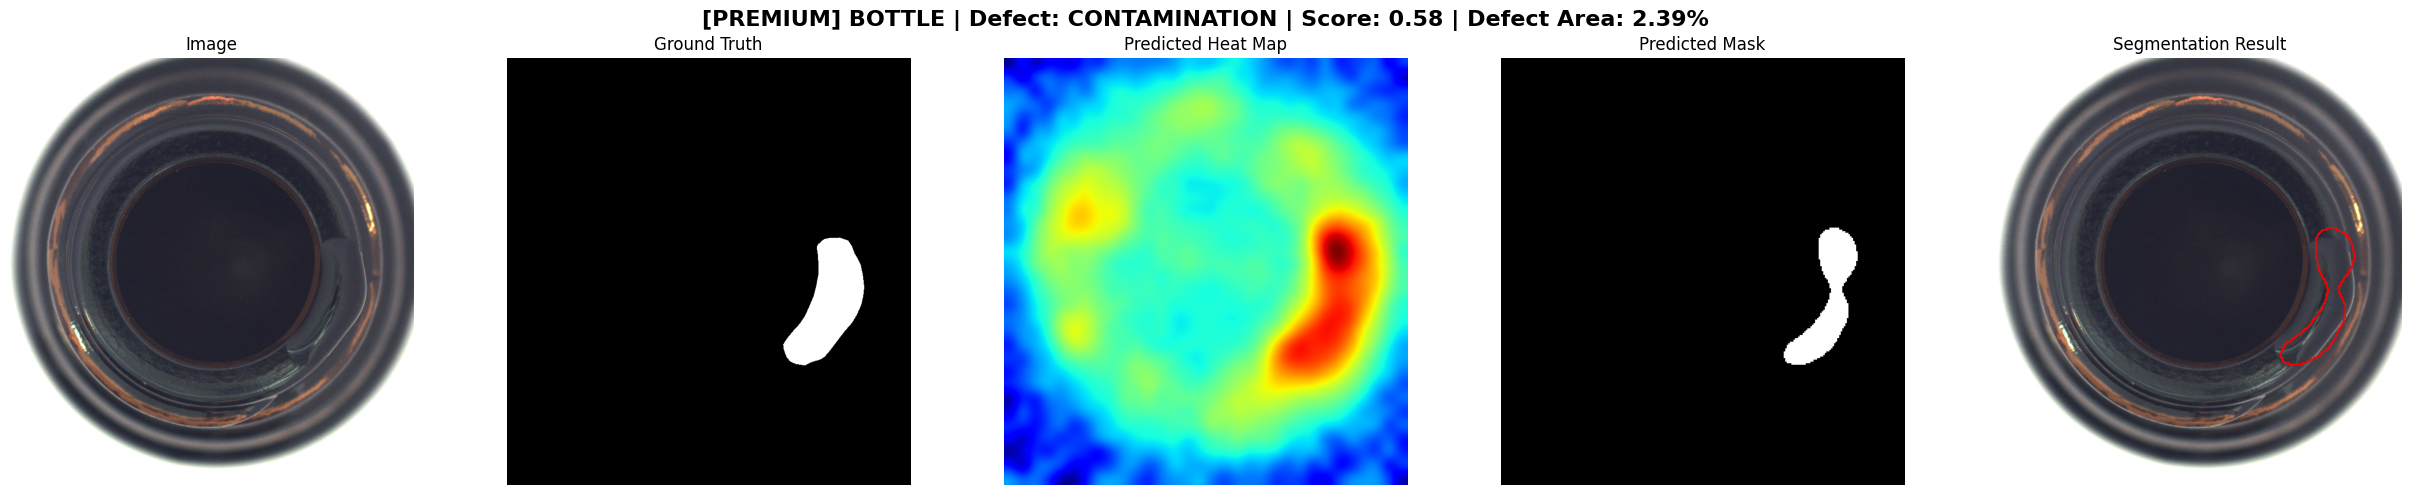
\includegraphics[width=0.95\textwidth]{img/fig16.png}%
	}
	\caption{ارزیابی ۵-پنلی کلاس بطری با مدل \lr{Wide\_ResNet50\_2}}
	\label{fig:bottle_resnet50}
\end{figure}


	در حالی که مدل پایه (\lr{ResNet-18}) در مواجهه با لکه آلودگی هلالی‌شکل، یک نقشه حرارتی پخش‌شده و نامنسجم تولید کرده و در نهایت دچار عدم مکان‌یابی (تولید ماسک کاملاً سیاه با مساحت خرابی \lr{0.00\%}) شده است، مدل پیشرفته (\lr{Wide\_ResNet50\_2}) با قاطعیت این ضعف را پوشش می‌دهد.
	
	مدل \lr{Wide\_ResNet50\_2} یک نقشه حرارتی بسیار متمرکز (\lr{Focal}) تولید کرده که انحنای لکه را دنبال می‌کند و با عبور موفق از آستانه قطعیت، ماسک باینری دقیقی (با مساحت \lr{2.39\%}) و منطبق بر \lr{Ground Truth} رسم می‌نماید.
	برتری معماری عریض‌تر در سرکوب نویزهای نوری مشهود است؛ برخلاف مدل پایه که فریب انعکاس نور روی لبه سالم شیشه را خورده و یک لکه حرارتی کاذب (\lr{Phantom Heat}) در سمت چپ تصویر ایجاد کرده بود، مدل پیشرفته با درک فضایی عمیق‌تر، این انعکاس طبیعی را نادیده گرفته و تمرکز پردازشی خود را منحصراً روی ناهنجاری ساختاری معطوف کرده است.


\subsubsection{مقایسه بصری عملکرد مدل‌ها در کلاس کابل (\lr{CABLE})}
شکل‌های \ref{fig:cable_resnet18} و \ref{fig:cable_resnet50} خروجی‌های ۵-پنلی این دو شبکه را نشان می‌دهند:

\begin{figure}[htbp]
	\centering
	\makebox[\textwidth][c]{%
		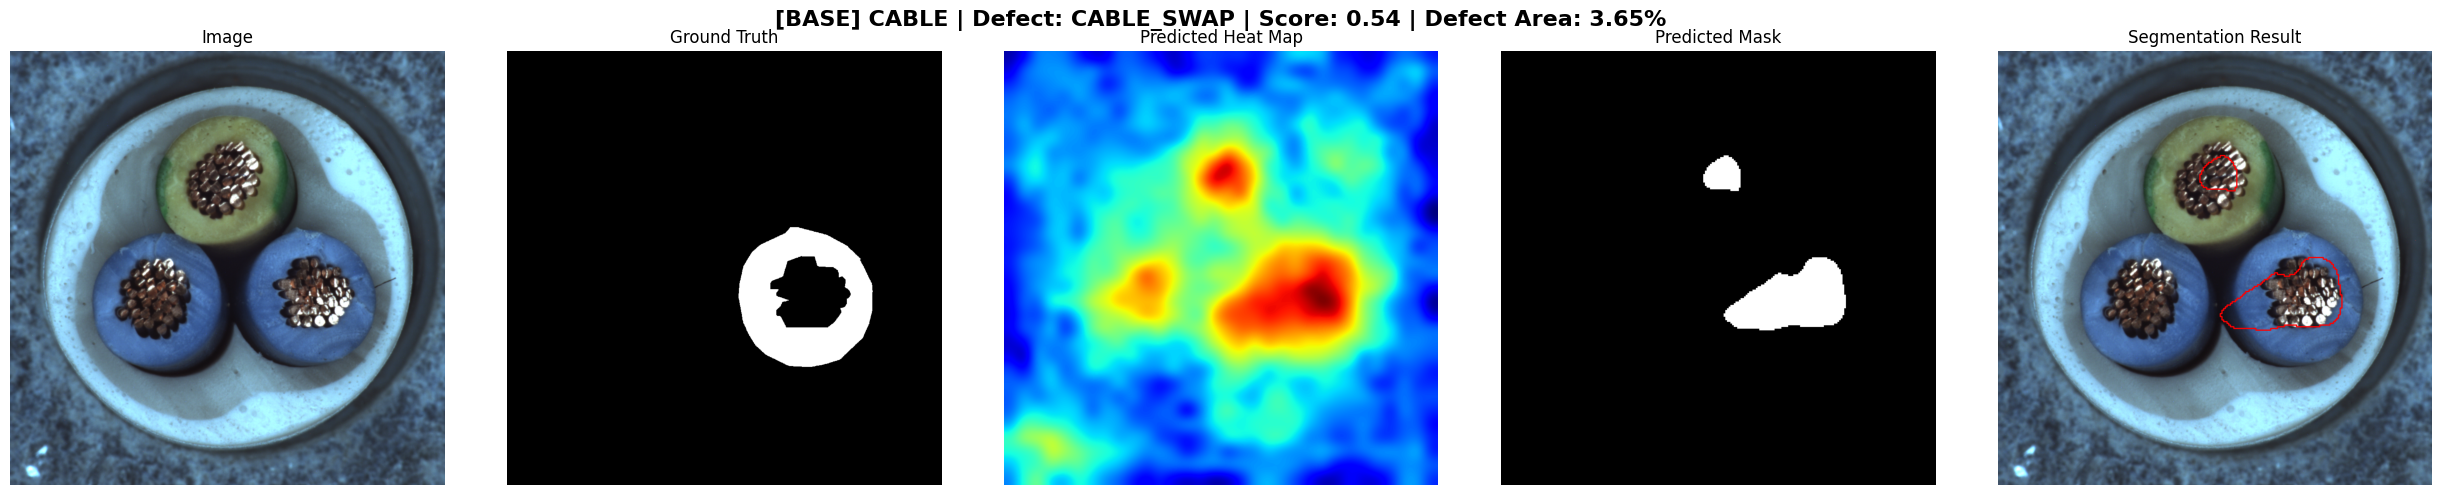
\includegraphics[width=0.95\textwidth]{img/fig17.png}%
	}
	\caption{ارزیابی ۵-پنلی کلاس کابل با مدل \lr{ResNet-18}}
	\label{fig:cable_resnet18}
\end{figure}

\begin{figure}[htbp]
	\centering
	\makebox[\textwidth][c]{%
		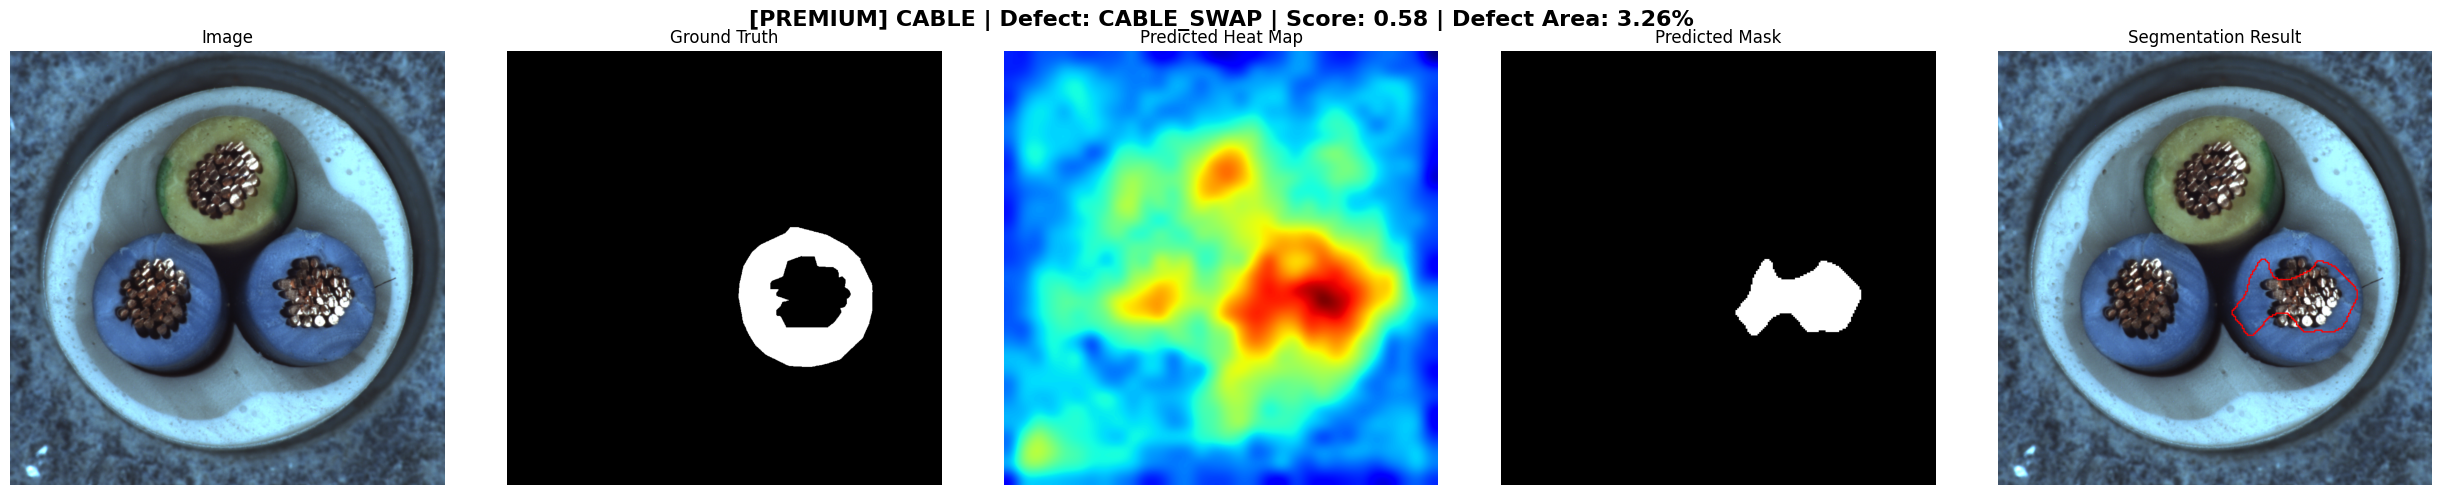
\includegraphics[width=0.95\textwidth]{img/fig18.png}%
	}
	\caption{ارزیابی ۵-پنلی کلاس کابل با مدل \lr{Wide\_ResNet50\_2}}
	\label{fig:cable_resnet50}
\end{figure}

در مواجهه با این جابه‌جایی رنگ‌ها، مدل \lr{BASE} (\lr{ResNet-18}) متوجه شده است که ترکیب کلی کابل غیرطبیعی است، اما در درک فضایی دقیق دچار سردرگمی شده است. نقشه حرارتی این مدل، تمرکز خود را از دست داده و سه لکه حرارتی مجزا تولید کرده است. نتیجه این عدم قطعیت در پنل ماسک پیش‌بینی‌شده و تصویر نهایی (\lr{Segmentation}) کاملاً مشهود است؛ شبکه علاوه بر سیم آبی‌رنگ پایین سمت راست، سیم سبزرنگ بالا را نیز به اشتباه به‌عنوان ناحیه معیوب علامت‌گذاری کرده است (یک خطای \lr{False Positive} در مکان‌یابی).

در مقابل، مدل \lr{PREMIUM} (\lr{Wide\_ResNet50\_2}) قدرت تحلیل بافتی (\lr{Contextual}) خود را به رخ می‌کشد. عرض بیشتر کانال‌ها در این معماری به شبکه اجازه داده تا رابطه فضایی بین رنگ‌ها را بهتر درک کند. این مدل موفق شده نویز و حرارت کاذب روی سیم بالایی را به‌شدت سرکوب کند و تمام قطعیت و تمرکز خود (هسته قرمز تیره در نقشه حرارتی) را منحصراً روی سیم پایین سمت راست (که برخلاف توزیع نرمال داده‌ها در آنجا قرار گرفته) جمع کند. در نتیجه، ماسک باینری \lr{ResNet-50} یکپارچه است و بدون اینکه اپراتور را با هشدارهای جانبی گیج کند، دقیقاً ناحیه مورد نظر \lr{Ground Truth} را هدف قرار داده است.

این مقایسه اثبات می‌کند که برای شناسایی خرابی‌های منطقی در محیط‌های شلوغ، ظرفیت بالاتر استخراج ویژگی در معماری‌های \lr{Wide}، از خطاهای مکان‌یابی به‌طور چشمگیری جلوگیری می‌کند.

\subsubsection{مقایسه بصری عملکرد مدل‌ها در کلاس مهره فلزی \lr{Metal\_Nut}}
در این کلاس طبق خروجی بخش \ref{subsec:RS50}، هر دو مدل عملکرد عالی داشتند و در بررسی پنل‌های خروجی، عدم تطابق و مورد اشتباهی برای مقایسه مشاهده نشد.

\subsubsection{مقایسه بصری عملکرد مدل‌ها در کلاس پیچ (\lr{SCREW})}

تحلیل مقایسه‌ای بصری تصاویر خروجی از کلاس پیچ (\lr{SCREW}) برای ناهنجاری از نوع دستکاری نوک پیچ (\lr{MANIPULATED\_FRONT})، چالش نویز بافتی (\lr{Textural Noise}) در مقیاس‌های میکروسکوپی را نشان می‌دهد. شکل‌های \ref{fig:screw_resnet18} و \ref{fig:screw_resnet50} خروجی‌های ۵-پنلی این دو شبکه را نشان می‌دهند:

\begin{figure}[htbp]
	\centering
	\makebox[\textwidth][c]{%
		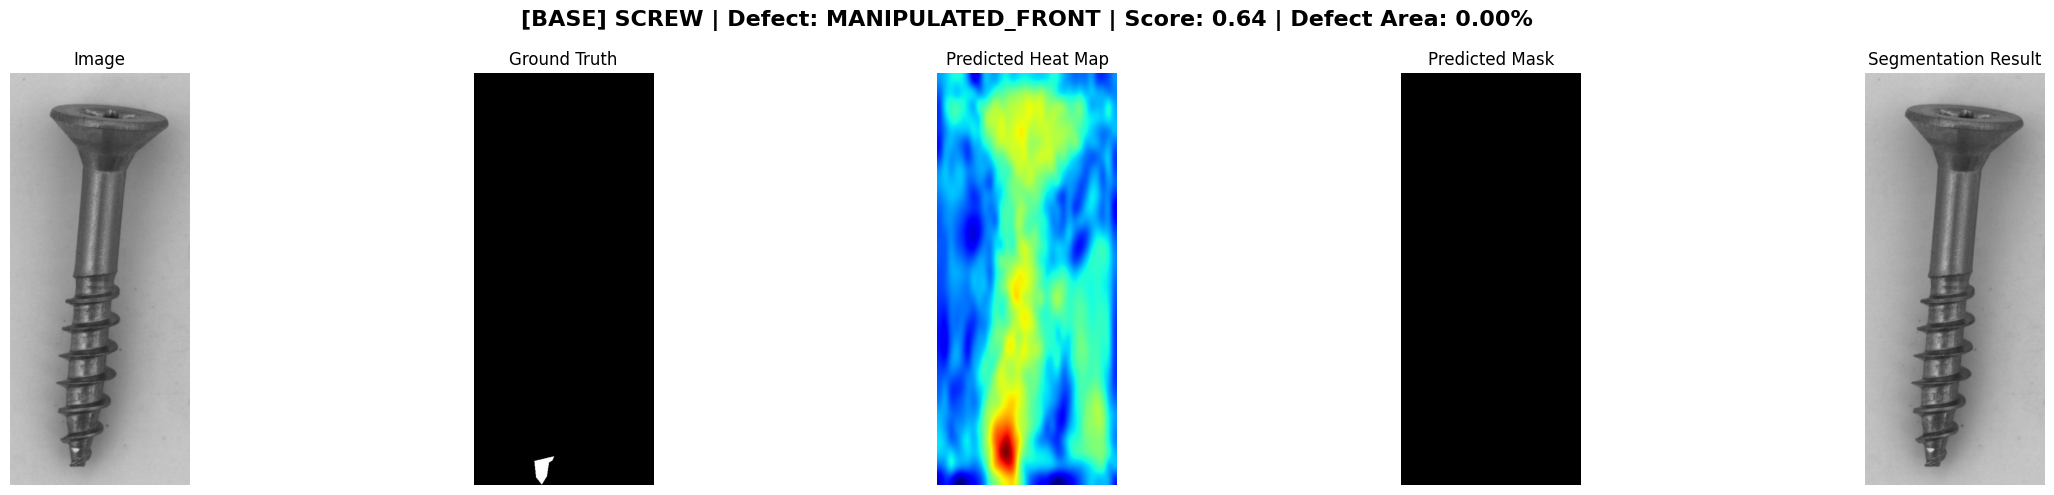
\includegraphics[width=0.95\textwidth]{img/fig19.png}%
	}
	\caption{ارزیابی ۵-پنلی کلاس پیچ با مدل \lr{ResNet-18}}
	\label{fig:screw_resnet18}
\end{figure}

\begin{figure}[htbp]
	\centering
	\makebox[\textwidth][c]{%
		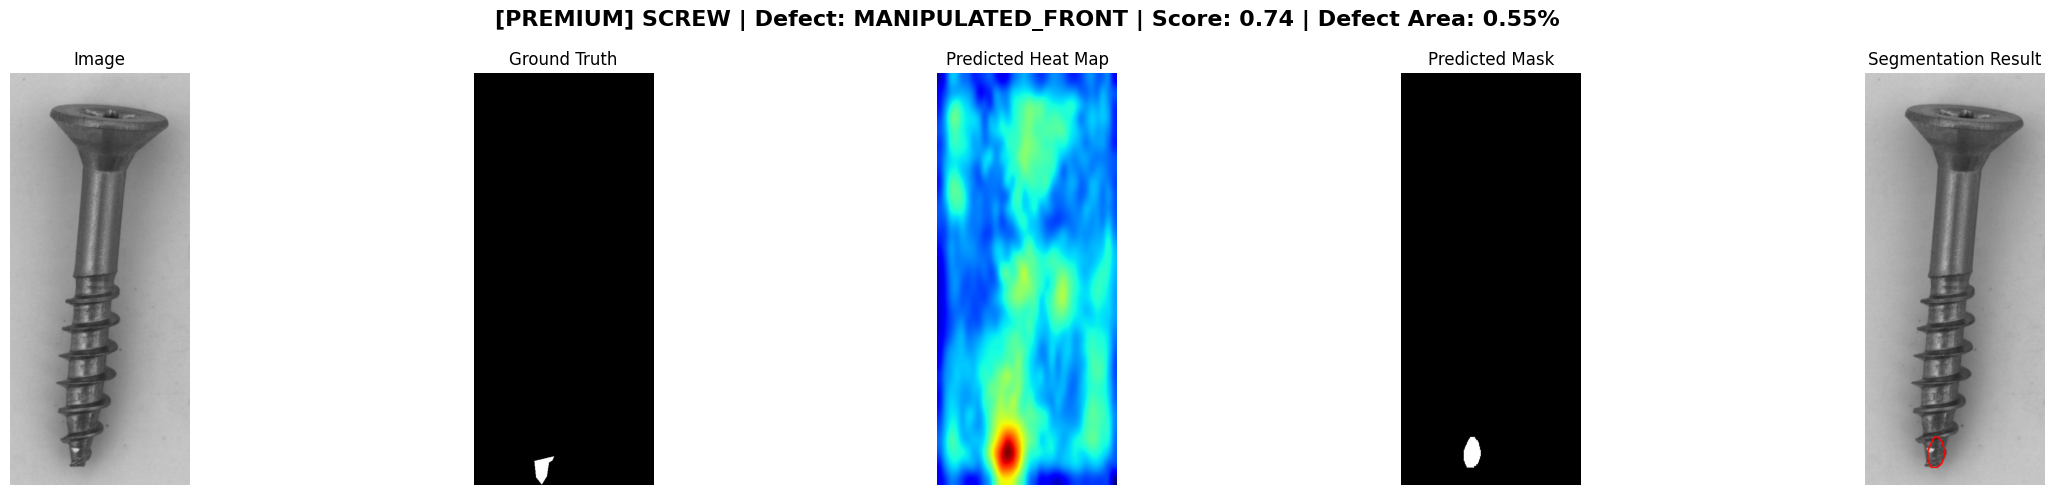
\includegraphics[width=0.95\textwidth]{img/fig20.png}%
	}
	\caption{ارزیابی ۵-پنلی کلاس پیچ با مدل \lr{Wide\_ResNet50\_2}}
	\label{fig:screw_resnet50}
\end{figure}

در شکل \ref{fig:screw_resnet18} (مدل پایه \lr{ResNet-18})، شاهد یک ناتوانی کلاسیک در فیلتر کردن نویز پس‌زمینه هستیم. رزوه‌های پیچ به دلیل داشتن سایه‌روشن‌های متوالی و ساختار هندسی پیچیده، برای شبکه‌های کم‌عمق‌تر یک چالش بزرگ محسوب می‌شوند. نقشه حرارتی مدل پایه به وضوح نشان می‌دهد که شبکه دچار سردرگمی شده است؛ اگرچه یک لکه قرمز در نوک پیچ دیده می‌شود، اما سراسر بدنه و گردن پیچ نیز با رنگ‌های زرد و سبز (حرارت کاذب) پوشیده شده است. این عدم قطعیت و توزیع پراکنده خطا باعث شده تا سیستم نتواند از آستانه تصمیم‌گیری (\lr{Threshold}) عبور کند و در نتیجه، دچار شکست مطلق در مکان‌یابی شده است (تولید ماسک کاملاً سیاه و مساحت خرابی \lr{0.00\%}).

در مقابل، شکل \ref{fig:screw_resnet50} (مدل پیشرفته \lr{Wide\_ResNet50\_2}) قدرت درک بافتی (\lr{Contextual Understanding}) شبکه‌های عریض‌تر را اثبات می‌کند. معماری پریمیوم توانسته است الگوی تکرارشونده و پیچیده رزوه‌های سالم را به‌طور کامل در بانک حافظه (\lr{Coreset}) خود به عنوان یک توزیع نرمال هضم و درک کند. در نتیجه، نقشه حرارتی این مدل، نویز روی بدنه پیچ را به‌شدت سرکوب کرده (رنگ‌های آبی سرد) و تمام انرژی پردازشی خود را در قالب یک هسته بسیار داغ و متمرکز، دقیقاً روی نوک آسیب‌دیده پیچ تخلیه کرده است. این وضوح سیگنال به نویز (\lr{SNR}) بالا، به رزنت ۵۰ اجازه داده تا با قاطعیت یک ماسک باینری بسیار ظریف (با مساحت تنها \lr{0.55\%}) استخراج کند که تطابق فضایی میلی‌متری و بی‌نقصی با ماسک \lr{Ground Truth} دارد.


\subsubsection{مقایسه بصری عملکرد مدل‌ها در کلاس مسواک و  \lr{ToothBrush}}
در این کلاس طبق خروجی بخش \ref{subsec:RS50}، هر دو مدل عملکرد عالی داشتند و در بررسی پنل‌های خروجی، عدم تطابق و مورد اشتباهی برای مقایسه مشاهده نشد، درست مانند کلاس مهره فلزی.
\subsubsection{مقایسه بصری عملکرد مدل‌ها در کلاس ترانزیستور (\lr{TRANSISTOR})}

تحلیل مقایسه‌ای بصری تصاویر خروجی از کلاس ترانزیستور (\lr{TRANSISTOR}) برای ناهنجاری از نوع شکستگی بدنه (\lr{DAMAGED\_CASE})، یکی از رایج‌ترین خطاهای سیستم‌های بینایی ماشین، یعنی هشدارهای کاذب موضعی (\lr{Localized False Positives}) را در مواجهه با قطعات فلزی و پس‌زمینه‌های شلوغ به تصویر می‌کشد. شکل‌های \ref{fig:transistor_resnet18} و \ref{fig:transistor_resnet50} خروجی‌های ۵-پنلی این دو شبکه را نشان می‌دهند:

\begin{figure}[htbp]
	\centering
	\makebox[\textwidth][c]{%
		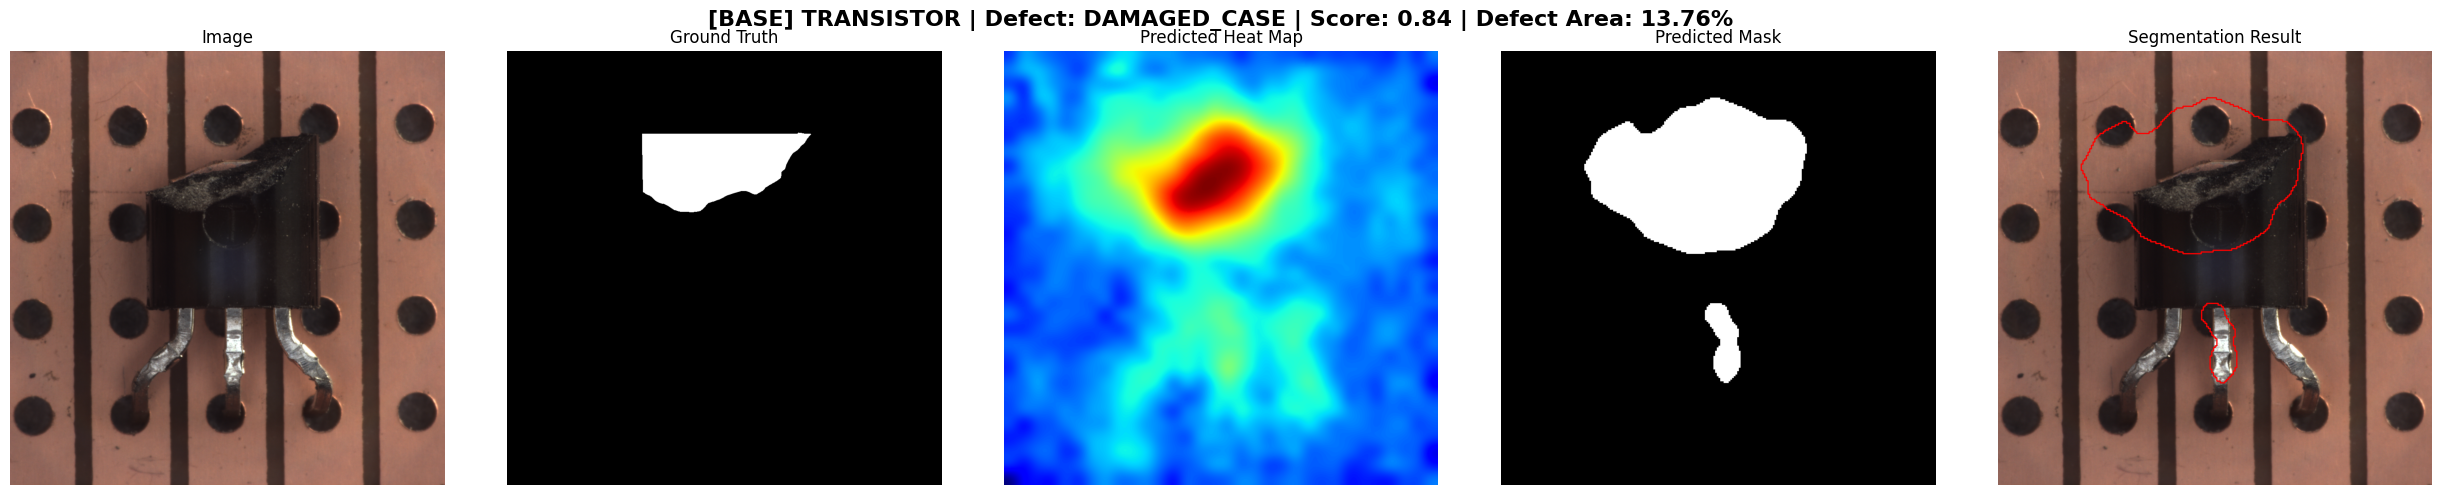
\includegraphics[width=0.95\textwidth]{img/fig21.png}%
	}
	\caption{ارزیابی ۵-پنلی کلاس ترانزیستور با مدل \lr{ResNet-18}}
	\label{fig:transistor_resnet18}
\end{figure}

\begin{figure}[htbp]
	\centering
	\makebox[\textwidth][c]{%
		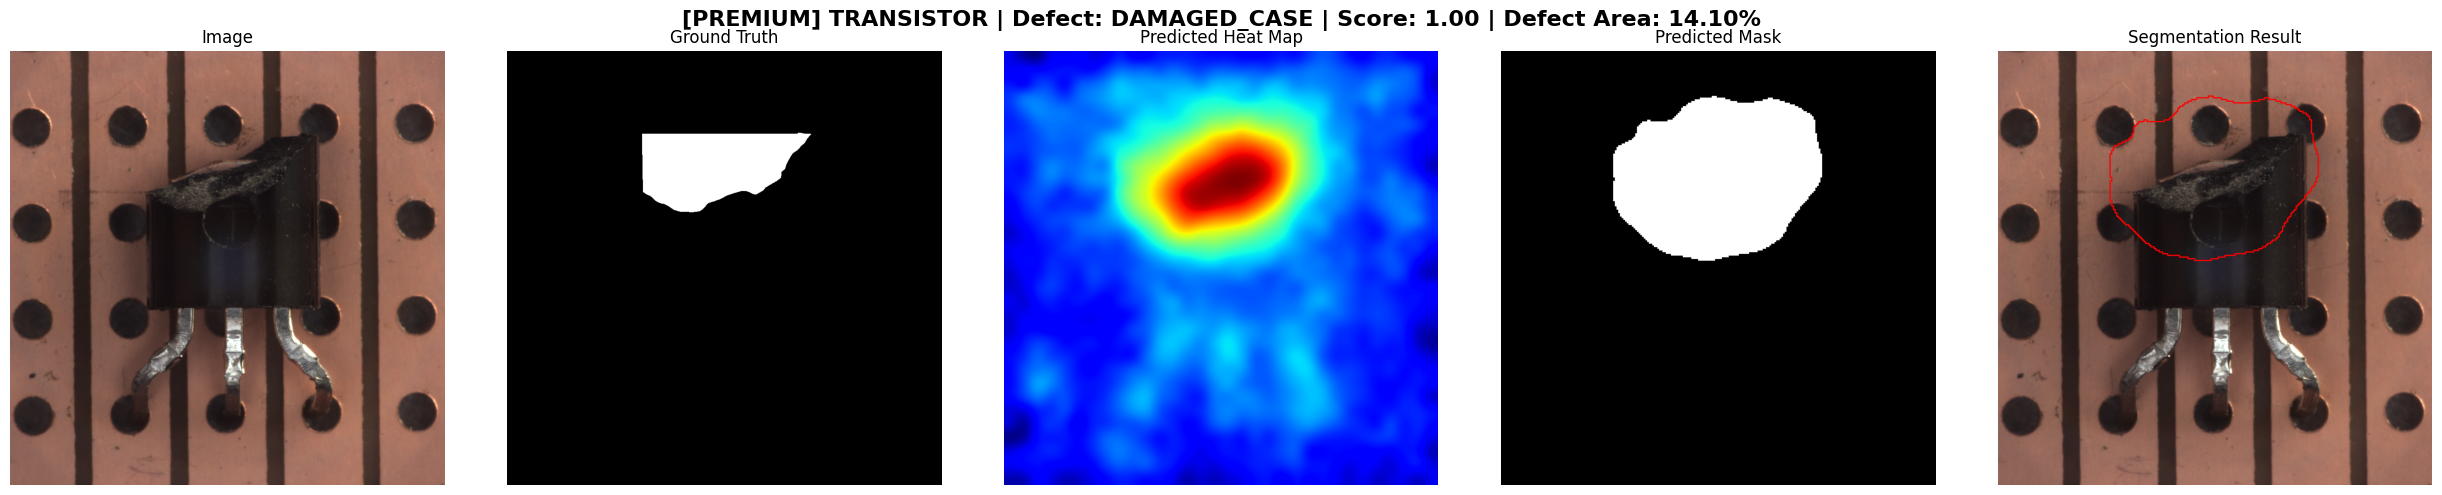
\includegraphics[width=0.95\textwidth]{img/fig22.png}%
	}
	\caption{ارزیابی ۵-پنلی کلاس ترانزیستور با مدل \lr{Wide\_ResNet50\_2}}
	\label{fig:transistor_resnet50}
\end{figure}

در شکل \ref{fig:transistor_resnet18} (مدل پایه \lr{ResNet-18})، اگرچه شبکه با موفقیت توانسته ناحیه اصلی شکستگی را در بالای ترانزیستور پیدا کند، اما در فیلتر کردن تغییرات طبیعی قطعه دچار مشکل شده است. در نقشه حرارتی این مدل، یک رد حرارتی زائد به سمت پایین کشیده شده است که نشان می‌دهد شبکه فریب بازتاب نور یا تغییرات جزئی لحیم‌کاری روی پین فلزی وسط را خورده است. این خطای ادراکی باعث شده تا در ماسک پیش‌بینی‌شده و تصویر نهایی (\lr{Segmentation Result})، علاوه بر ناحیه اصلی، یک لکه کوچک و کاذب نیز روی پایه ترانزیستور به‌عنوان خرابی علامت‌گذاری شود. در یک خط تولید واقعی، این هشدارهای جانبی می‌توانند باعث سردرگمی اپراتور یا افت اعتماد به سیستم (\lr{System Trust}) شوند.

در طرف مقابل، خروجی شکل \ref{fig:transistor_resnet50} (مدل پیشرفته \lr{Wide\_ResNet50\_2}) یک نمونه عالی از مقاومت بافتی (\lr{Contextual Robustness}) است. معماری عریض‌تر با درک عمیق‌تر از متریال‌های مختلف، به‌خوبی آموخته است که نوسانات نوری روی پین‌های فلزی، جزئی از توزیع نرمال این قطعه هستند. در نتیجه، نقشه حرارتی در مدل پریمیوم کاملاً از نویزهای روی پایه‌ها پاکسازی شده (رنگ آبی تیره) و سیستم تمام قطعیت خود (با امتیاز کامل \lr{1.00}) را منحصراً روی ناهنجاری ساختاری پلاستیک بدنه متمرکز کرده است. ماسک باینری تولیدشده در این حالت کاملاً یکپارچه، تمیز و بدون هیچ‌گونه آرتیفکت (\lr{Artifact}) اضافی است که برتری مطلق مدل سنگین‌تر را در محیط‌های دارای پس‌زمینه شلوغ (مانند سوراخ‌های مدار چاپی) اثبات می‌کند.


\section{بسته‌بندی و آمادگی برای استقرار (\lr{Packaging \& Deployment Readiness})}


در محیط‌های صنعتی واقعی، کامپیوترهای متصل به بازوهای رباتیک یا دوربین‌های نوار نقاله (\lr{Edge Devices}) معمولاً فاقد محیط‌های برنامه‌نویسی سنگین، کتابخانه‌هایی مانند \lr{Anomalib}، یا حتی زبان پایتون هستند. به همین دلیل است که در پایان مرحله آموزش، مدل‌ها را با فرمت \lr{TorchScript} (فایل‌های \lr{.pt}) اکسپورت کردیم.

فایل \lr{.pt} یک گراف محاسباتی کاملاً مستقل است که تمام وزن‌ها، ساختار شبکه (\lr{ResNet-18}) و حتی پیش‌پردازش‌های اولیه را در دل خود جای داده است. هدف این اسکریپت در \lr{Stage 6}، جمع‌آوری خودکار این مغزهای مصنوعی و بسته‌بندی آن‌ها برای انتقال ایمن به سخت‌افزارهای صنعتی است.

این اسکریپت با ظرافت و رعایت استانداردهای اتوماسیون نوشته شده است تا هیچ فایل اضافی یا سنگینی وارد پکیج نهایی نشود:


دستور \lr{\texttt{glob.glob(..., '*.pt')}} یک انتخاب مهندسی بسیار دقیق است. سیستم به جای برداشتن فایل‌های سنگین چک‌پوینت (\lr{.ckpt} که فقط برای ادامه آموزش کاربرد دارند)، در تمام زیرپوشه‌ها جستجو کرده و فقط و فقط فایل‌های کامپایل‌شده استقرار (\lr{\texttt{model.pt}}) را جمع‌آوری می‌کند. این کار حجم فایل نهایی را به‌شدت بهینه نگه می‌دارد.

در بلوک ساخت \lr{ZIP}، استفاده از \lr{\texttt{os.path.relpath}} بسیار حیاتی است. این دستور تضمین می‌کند که فایل‌های \lr{.pt} در یک پوشه درهم‌ریخته (\lr{Flat}) روی هم ریخته نشوند. سیستم نام کلاس‌ها (مانند \lr{cable} یا \lr{bottle}) را به عنوان پوشه والد در فایل زیپ حفظ می‌کند تا نرم‌افزار نهایی کارخانه، دقیقاً بداند هر فایل وزن مربوط به کدام قطعه است.


دستور \lr{\texttt{files.download(ZIP\_NAME)}} حلقه اتصال کلود به لوکال است و به صورت خودکار، فایل تجمیع‌شده را به سیستم منتقل می‌کند.


لاگ‌های خروجی حاصل از اجرای اسکریپت بسته‌بندی به شرح زیر است:


\begin{tcolorbox}[colback=Tan!15, colframe=MidnightBlue]
	\begin{latin}
		\begin{verbatim}
--- Stage 6: Packaging Base Industrial Models (ResNet-18) ---
Found 6 production-ready BASE models. Zipping now...

cable/Patchcore/MVTecAD/cable/v2/weights/torch/model.pt
bottle/Patchcore/MVTecAD/bottle/v0/weights/torch/model.pt
metal_nut/Patchcore/MVTecAD/metal_nut/v0/weights/torch/model.pt
screw/Patchcore/MVTecAD/screw/v0/weights/torch/model.pt
toothbrush/Patchcore/MVTecAD/toothbrush/v0/weights/torch/model.pt
transistor/Patchcore/MVTecAD/transistor/v0/weights/torch/model.pt

Packaging Complete! File saved as: /content/Factory_AI_Brains_
Base_ResNet18.zip
		\end{verbatim}
	\end{latin}
\end{tcolorbox}



پیام \lr{Found 6 production-ready BASE models} تایید می‌کند که موتور آموزش روی تمام ۶ کلاس هدف (بطری، کابل، مهره فلزی، پیچ، مسواک و ترانزیستور) با موفقیت اجرا شده و برای هر کدام یک گراف محاسباتی مستقل و بی‌نقص تولید کرده است.
پایان عملیات و تولید فایل \lr{\texttt{Factory\_AI\_Brains\_Base\_ResNet18.zip}} اکنون حاوی فایل های آموزش‌دیده است. 



\section{شبیه‌سازی}

\begin{figure}[H]
	\centering
	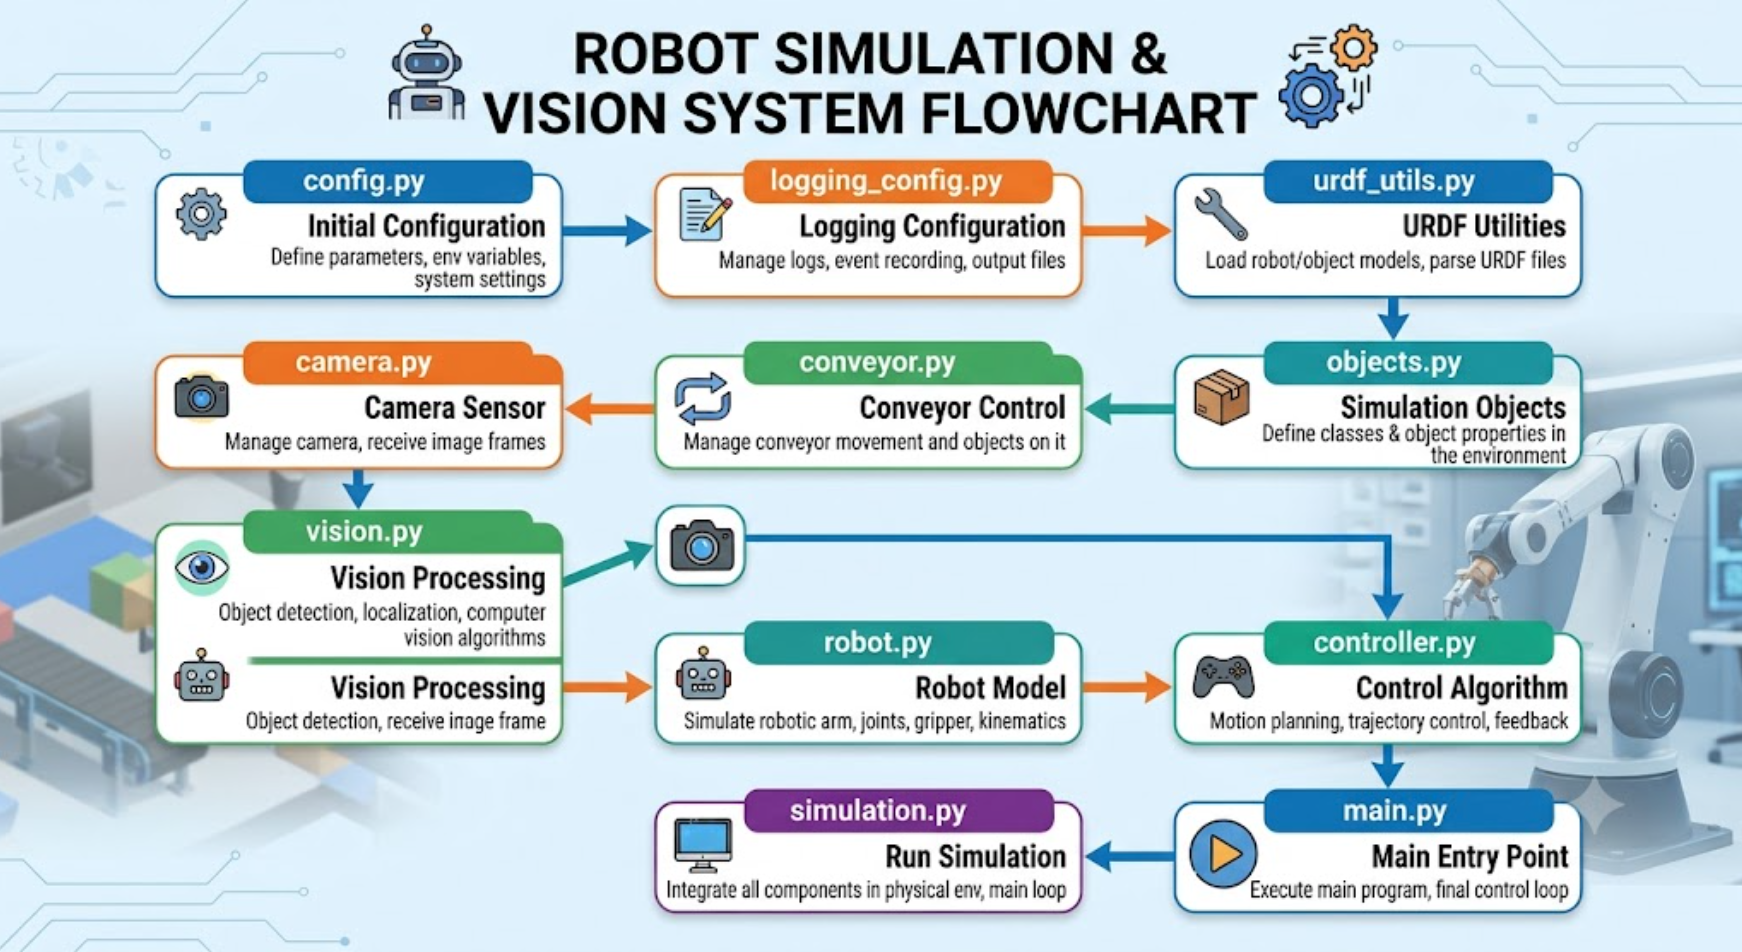
\includegraphics[width=0.85\textwidth]{img/fig33.png}
	\caption{فلوچارت ماژول‌‌های شبیه‌سازی}
	\label{fig:fig33}
\end{figure}
\subsection{مستندسازی بخش شبیه‌سازی: ماژول \lr{config.py}}

\subsubsection{معرفی ماژول}
ماژول \lr{config.py} به‌عنوان هسته مرکزی تنظیمات (\lr{Central Configuration}) برای شبیه‌سازی همزاد دیجیتال (\lr{Digital Twin}) در محیط \lr{PyBullet} عمل می‌کند. این فایل میزبان یک کلاس استاتیک به نام \lr{Config} است که تمامی ثابت‌های قابل تنظیم مربوط به شبیه‌سازی فیزیکی، مکانیزم‌های مکانیکی، سیستم اپتیک دوربین و پایپ‌لاین بینایی ماشین را در خود جای داده است.

\subsubsection{هدف طراحی}
هدف اصلی از طراحی این ماژول، پیاده‌سازی الگوی معماری «منبع واحد حقیقت» (\lr{Single Source of Truth}) برای پارامترهای سیستم است. در سیستم‌های پیچیده رباتیک و شبیه‌سازی، پراکندگی اعداد ثابت (\lr{Magic Numbers}) در فایل‌های مختلف باعث کاهش خوانایی کد و افزایش خطای انسانی در فرآیند تنظیم دقیق (\lr{Fine-tuning}) می‌شود. با تجمیع تمامی پارامترها در این کلاس، امکان کالیبراسیون و تغییر رفتار کل سیستم تنها از یک نقطه متمرکز فراهم شده است.

\subsubsection{نقش ماژول در کل سیستم}
این ماژول نقش تنظیم‌کننده (\lr{Regulator}) کل شبیه‌سازی را بر عهده دارد. از نرخ به‌روزرسانی موتور فیزیک گرفته تا مختصات سینماتیکی بازوی ربات، فواصل کانونی دوربین و آستانه‌های حساسیت در شبکه‌های عصبی تشخیص عیب، همگی توسط این کلاس به سایر ماژول‌ها دیکته می‌شوند. این ساختار اجازه می‌دهد تا توسعه‌دهنده بدون نیاز به درک یا تغییر منطق داخلی سایر فایل‌ها، سناریوهای مختلف شبیه‌سازی را پیکربندی کند.

\subsubsection{ساختار کلی و اجزای مهم}
کلاس \lr{Config} به‌صورت منطقی به چند بخش اصلی تقسیم شده است:

\begin{itemize}
	\item پارامترهای شبیه‌سازی و فیزیک (\lr{Simulation}): شامل وضعیت رابط کاربری (\lr{GUI})، شتاب گرانش (\lr{-9.81})، تعداد گام‌های شبیه‌سازی (۶۰۰۰ گام برای اجرای طولانی‌تر دمو) و از همه مهم‌تر، گام زمانی (\lr{Time Step}) که روی \lr{1/240} ثانیه تنظیم شده است؛ این مقدار استاندارد موتور \lr{PyBullet} برای محاسبه دقیق دینامیک صلب است.
	
	\item مشخصات نوار نقاله (\lr{Conveyor}): ابعاد هندسی (طول، عرض، ارتفاع)، سرعت حرکت پیش‌فرض (\lr{0.5} متر بر ثانیه) و موقعیت قرارگیری آن در فضای سه‌بعدی را تعریف می‌کند.
	
	\item مختصات بازوی رباتیک (\lr{Robot Arm}): شامل موقعیت نصب پایه ربات و نقاط کلیدی عملیاتی از جمله نقطه برداشتن قطعه (\lr{Pick}) و نقاط رهاسازی برای دو مسیر متفاوت تعمیر (\lr{Repair}) و ضایعات (\lr{Scrap}). این مختصات پایه و اساس حل معادلات سینماتیک معکوس (\lr{Inverse Kinematics}) در ماژول ربات خواهند بود.
	
	\item اپتیک و دوربین (\lr{Camera}): پارامترهای رندرینگ شامل وضوح تصویر (۳۲۰ در ۳۲۰ پیکسل)، زاویه دید (\lr{FOV}) برابر با ۳۵ درجه، و سطوح برش مقطع (\lr{Near/Far clipping planes}). موقعیت استراتژیک دوربین به گونه‌ای تنظیم شده است (مقدار \lr{X} برابر با \lr{-1.5}) که تصویربرداری و استنتاج مدل پیش از رسیدن قطعه به گیت‌های تصمیم‌گیری انجام شود.
	
	\item تولید قطعات (\lr{Object Spawning}): فاصله زمانی بین تولید هر قطعه روی نوار نقاله که با توجه به فرکانس ۲۴۰ هرتز، روی ۳۵۰ گام (حدود ۱.۴۵ ثانیه) تنظیم شده است تا قطعات با فاصله فیزیکی مناسبی از یکدیگر قرار گیرند.
	
	\item پایپ‌لاین استنتاج هوش مصنوعی (\lr{Vision Pipeline}): این بخش حیاتی، نحوه ارتباط شبیه‌ساز با مدل‌های آموزش‌دیده را مشخص می‌کند. شامل مسیر فایل وزن‌های \lr{YOLOv8} (\lr{best.pt})، مسیر مدل‌های تشخیص ناهنجاری (\lr{PatchCore/ResNet-18}) و آستانه‌های تصمیم‌گیری است.
\end{itemize}

\subsubsection{نحوه عملکرد}
از آنجا که تمامی مقادیر به‌عنوان ویژگی‌های کلاس (\lr{Class Attributes}) تعریف شده‌اند، این پارامترها در حافظه به صورت استاتیک بارگذاری می‌شوند. سایر ماژول‌ها می‌توانند مستقیماً از طریق فراخوانی نام کلاس (مانند \lr{Config.CONVEYOR\_SPEED\_DEFAULT}) یا از طریق ایجاد یک نمونه از آن، به مقادیر دسترسی پیدا کنند.

در بخش هوش مصنوعی، عملکرد سیستم با ترکیب دو آستانه (\lr{Threshold}) کنترل می‌شود:

\begin{itemize}
	\item آستانه تشخیص ناهنجاری (\lr{ANOMALY\_CONFIDENCE\_THRESHOLD}): روی مقدار \lr{0.7} تنظیم شده است؛ به این معنا که اگر خروجی مدل \lr{PatchCore} اطمینانی برابر یا بیشتر از ۷۰ درصد به وجود عیب داشته باشد، قطعه وارد فاز بررسی مساحت نقص می‌شود.
	
	\item آستانه تصمیم‌گیری استراتژیک (\lr{DEFECT\_AREA\_SCRAP\_THRESHOLD}): اگر مساحت ناحیه معیوب بیش از ۱۵ درصد (\lr{0.15}) از کل قطعه باشد، فرمان انتقال به سبد ضایعات (\lr{Scrap}) صادر می‌شود؛ در غیر این صورت، قطعه به مسیر تعمیر (\lr{Repair}) هدایت می‌گردد.
\end{itemize}

\subsubsection{ارتباط با سایر ماژول‌ها}
این فایل عملاً وابستگی وارداتی (\lr{Import}) به جز کتابخانه \lr{os} برای مسیردهی ندارد، اما در تمام ماژول‌های دیگر وارد (\lr{Import}) می‌شود.

\begin{itemize}
	\item ماژول‌های \lr{robot.py} و \lr{conveyor.py} برای دریافت ابعاد و مختصات حرکتی.
	\item ماژول \lr{camera.py} برای دریافت ماتریس‌های پروجکشن و تنظیمات رندر.
	\item ماژول \lr{vision.py} برای بارگذاری وزن‌های شبکه عصبی (مانند \lr{best.pt} که در فاز قبلی آموزش داده شده بود) و اعمال آستانه‌های تصمیم‌گیری تصویر.
	\item ماژول‌های \lr{main.py} و \lr{simulation.py} برای مدیریت حلقه اصلی و زمان‌بندی تولید اشیاء (\lr{Spawning}).
\end{itemize}

\subsubsection{جمع‌بندی}
ماژول \lr{config.py} با پیاده‌سازی یک معماری ماژولار و متمرکز، مدیریت پیچیدگی‌های شبیه‌ساز همزاد دیجیتال را بسیار ساده کرده است. تعریف دقیق مرزهای فیزیکی، مختصات سینماتیکی و آستانه‌های استنتاج یادگیری عمیق در این فایل، تضمین می‌کند که سیستم برای انجام تست‌های مختلف (مانند تغییر سرعت نوار نقاله یا تنظیم حساسیت مدل تشخیص عیب) نیازی به بازنویسی کدهای عملیاتی نداشته باشد و از یک استاندارد مهندسی نرم‌افزار سطح بالا پیروی کند.

\subsection{مستندسازی بخش شبیه‌سازی: ماژول \lr{logging\_config.py}}

\subsubsection{معرفی ماژول}
ماژول \lr{logging\_config.py} سیستم یکپارچه و متمرکز ثبت وقایع (\lr{Centralized Logging}) را برای کل پروژه شبیه‌سازی همزاد دیجیتال (\lr{Digital Twin}) پیکربندی می‌کند. با وارد کردن این ماژول، ساختار پایه لاگ‌گیری تنها برای یک‌بار در حافظه تنظیم شده و یک نمونه مشترک (\lr{Shared Instance}) از لاگر برای استفاده در سراسر پروژه در دسترس قرار می‌گیرد.

\subsubsection{هدف طراحی}
در توسعه سیستم‌های پیچیده مهندسی و نرم‌افزارهای رباتیک، استفاده از دستورهای ساده چاپ در کنسول (مانند \lr{print}) برای مانیتورینگ و خطایابی سیستم ناکارآمد است؛ زیرا فاقد اطلاعات حیاتی مانند برچسب زمانی، سطح اهمیت پیام و قابلیت ذخیره‌سازی ساختاریافته هستند. هدف از طراحی این ماژول، جایگزینی رویکردهای غیرساختاریافته با یک سیستم استاندارد، یکپارچه و قابل ردیابی است تا تمامی گزارش‌های خروجی از بخش‌های مختلف برنامه با قالبی کاملاً یکسان تولید شوند.

\subsubsection{نقش ماژول در کل سیستم}
این ماژول نقش سیستم عصبی گزارش‌دهی را در شبیه‌ساز ایفا می‌کند. ثبت وضعیت رویدادهای فیزیکی، زمان‌بندی دقیق عکس‌برداری‌های دوربین (\lr{Camera Shots})، و از همه مهم‌تر، مانیتورینگ نتایج استنتاج مدل‌های بینایی ماشین (\lr{Vision Inference Results}) از طریق این ساختار انجام می‌شود. این یکپارچگی به توسعه‌دهنده اجازه می‌دهد تا در زمان اجرای شبیه‌سازی، رفتار کل سیستم را به صورت بلادرنگ (\lr{Real-time}) و با جزئیات دقیق زیر نظر داشته باشد.

\subsubsection{ساختار کلی و اجزای مهم}
این ماژول با استفاده از کتابخانه استاندارد \lr{logging} در پایتون بنا شده و شامل دو بخش کلیدی است:

\begin{itemize}
	\item پیکربندی پایه (\lr{logging.basicConfig}): در این بخش سطح ثبت وقایع روی \lr{INFO} تنظیم شده است؛ بدین معنا که اطلاعات جریان عادی برنامه، هشدارها و خطاها ثبت می‌شوند. همچنین فرمت پیام‌ها به‌صورت \lr{\%(asctime)s [\%(levelname)s] \%(message)s} تعریف شده است که به ترتیب، برچسب زمانی دقیق (\lr{Timestamp})، سطح اهمیت پیام (مثلاً \lr{INFO} یا \lr{ERROR}) و متن اصلی پیام را در بر می‌گیرد.
	
	\item فضای نام اختصاصی (\lr{logging.getLogger}): یک شیء لاگر با نام اختصاصی \lr{"DigitalTwin"} ایجاد می‌شود. این کار باعث می‌شود تمام لاگ‌های صادر شده از این سیستم، دارای یک هویت مشخص (\lr{Namespace}) باشند که در صورت ترکیب با سیستم‌های نرم‌افزاری دیگر، تفکیک آن‌ها به سادگی امکان‌پذیر باشد.
\end{itemize}

\subsubsection{نحوه عملکرد}
عملکرد این ماژول بر پایه مفهوم بارگذاری یک‌باره (\lr{Run-once Configuration}) در پایتون استوار است. زمانی که اولین ماژول در پروژه این فایل را بارگذاری (\lr{Import}) می‌کند، تابع \lr{basicConfig} اجرا شده و قالب‌بندی در سطح ریشه (\lr{Root}) تنظیم می‌شود. سپس شیء \lr{logger} ایجاد شده و در اختیار برنامه قرار می‌گیرد. در فراخوانی‌های بعدی توسط سایر ماژول‌ها، پیکربندی مجدداً اجرا نمی‌شود، بلکه همان نمونه \lr{logger} ایجاد شده به آن‌ها پاس داده می‌شود (شبیه‌سازی مفهوم الگوی طراحی \lr{Singleton}).

\subsubsection{ارتباط با سایر ماژول‌ها}
این فایل یک ماژول زیربنایی (\lr{Infrastructure Module}) است و وابستگی به هیچ یک از فایل‌های داخلی پروژه ندارد، اما خود در اکثر ماژول‌های سیستم وارد (\lr{Import}) می‌شود:

\begin{itemize}
	\item در ماژول \lr{vison.py}: برای ثبت نتایج پردازش تصویر، کلاس‌های تشخیص داده شده و مقادیر اطمینان (\lr{Confidence Scores}).
	\item در ماژول‌های \lr{simulation.py} و \lr{main.py}: برای گزارش‌دهی از چرخه حیات شبیه‌سازی، مانند زمان تولید اشیاء جدید یا شروع و پایان فرآیندها.
	\item در ماژول \lr{camera.py}: برای لاگ‌گیری از وضعیت ثبت فریم‌ها.
\end{itemize}

\subsubsection{جمع‌بندی}
ماژول \lr{logging\_config.py} با وجود حجم بسیار کمِ کد، ارزش مهندسی بالایی به سیستم شبیه‌سازی می‌افزاید. این فایل با استانداردسازی جریان خروجی اطلاعات، فرآیند مانیتورینگ، دیباگینگ و تحلیل عملکرد مدل‌های هوش مصنوعی در تعامل با محیط فیزیکی را به شکل چشم‌گیری تسهیل کرده و خروجی‌های متنی پروژه را به استانداردهای نرم‌افزارهای صنعتی نزدیک می‌کند.

\subsection{مستندسازی بخش شبیه‌سازی: ماژول \lr{urdf\_utils.py}}

\subsubsection{معرفی ماژول}
ماژول \lr{urdf\_utils.py} به‌عنوان موتور تولید رویه‌ای دارایی‌ها (\lr{Procedural Asset Generation}) در شبیه‌ساز عمل می‌کند. این فایل شامل مجموعه‌ای از توابع کمکی است که وظیفه دارند فایل‌های سه‌بعدی استاندارد مانند \lr{URDF} (\lr{Unified Robot Description Format}) و \lr{OBJ} را در زمان اجرا (\lr{Runtime}) به‌صورت پویا تولید و روی دیسک ذخیره کنند تا بلافاصله توسط موتور فیزیک \lr{PyBullet} بارگذاری شوند.

\subsubsection{هدف طراحی}
در توسعه نرم‌افزارهای رباتیک، وابستگی به فایل‌های استاتیک \lr{CAD} و \lr{URDF} می‌تواند چالش‌هایی در زمینه انتقال‌پذیری پروژه (\lr{Portability}) و مدیریت مسیر فایل‌ها ایجاد کند. هدف اصلی از طراحی این ماژول، حذف نیاز به حمل فایل‌های جانبی استاتیک در کنار کدهای پروژه است. با استفاده از این رویکرد، سیستم می‌تواند اجزای محیطی و فیزیکی خود را دقیقاً در زمان اجرای برنامه با پارامترهای مشخص بسازد. علاوه بر این، این ماژول یک محدودیت ذاتی در موتور \lr{PyBullet} پیرامون نحوه نگاشت بافت (\lr{Texture Mapping}) را با تولید یک فایل هندسی اختصاصی حل می‌کند.

\subsubsection{نقش ماژول در کل سیستم}
این ماژول نقش «کارخانه سازنده» زیرساخت‌های فیزیکی و بصری محیط شبیه‌سازی را بر عهده دارد. پایه‌های دوربین، ابزار مجری نهایی (\lr{End-effector}) ربات، سبدهای جمع‌آوری قطعات (\lr{Repair/Scrap}) و صفحات بصری حاوی تصویر قطعات، همگی توسط این ماژول متولد می‌شوند. در واقع، این فایل رابطی میان منطق برنامه‌نویسی و موتور فیزیکی برای تعریف هندسه، جرم، اصطکاک و ساختار سینماتیکی اشیاء محیطی است.

\subsubsection{ساختار کلی و اجزای مهم}
این ماژول از چهار تابع کلیدی تشکیل شده است که هر کدام وظیفه مهندسی مشخصی دارند:

\begin{itemize}
	\item \lr{\texttt{create\_camera\_stand\_urdf}}: سازنده ساختار سینماتیکی پایه دوربین.
	\item \lr{\texttt{create\_magnetic\_tool\_urdf}}: سازنده ابزار مغناطیسی متصل به بازوی ربات.
	\item \lr{\texttt{create\_bucket}}: تولیدکننده فیزیکی سبدهای مرتب‌سازی با استفاده از \lr{API} مستقیم \lr{PyBullet}.
	\item \lr{\texttt{create\_textured\_plane\_obj}}: سازنده یک شبکه هندسی (\lr{Mesh}) مسطح و سفارشی برای نگاشت دقیق تصاویر روی قطعات.
\end{itemize}

\subsubsection{نحوه عملکرد}
عملکرد این ماژول بر پایه دو مکانیزم متفاوت استوار است: تولید فایل متنی (\lr{XML/OBJ}) و ایجاد مستقیم اشیاء چندتکه‌ای (\lr{MultiBody}) در موتور فیزیک.

\begin{itemize}
	\item مدل‌سازی سینماتیکی (\lr{URDF Generation}): توابع مربوط به دوربین و ابزار مغناطیسی، یک ساختار درختی از اتصالات (\lr{Joints}) و پیوندها (\lr{Links}) را به زبان \lr{XML} تولید می‌کنند. به عنوان مثال، در پایه دوربین، چهار پیوند مختلف (\lr{base}، \lr{pole}، \lr{arm}، \lr{camera\_body}) با استفاده از مفاصل ثابت (\lr{type="fixed"}) به یکدیگر متصل می‌شوند تا یک جسم صلب یکپارچه را تشکیل دهند. تنظیم جرم (\lr{mass value="0"}) در پایه دوربین، آن را از نظر دینامیکی در محیط فیکس می‌کند.
	
	\item ایجاد سبدهای فیزیکی (\lr{Physical Buckets}): تابع \lr{\texttt{create\_bucket}} به جای تولید فایل خارجی، مستقیماً از توابع سطح پایین موتور فیزیک استفاده می‌کند. این تابع یک کف و چهار دیواره را به‌عنوان یک جسم واحد (\lr{MultiBody}) می‌سازد. یک نکته ظریف مهندسی در این بخش، تنظیم ارتفاع متفاوت دیواره‌هاست؛ دیواره جلویی (\lr{Front lip}) کوتاه‌تر در نظر گرفته شده تا ورود قطعات به سبد تسهیل شود. همچنین، تنظیم جرم پایه برابر صفر (\lr{baseMass=0}) مانع از حرکت یا واژگونی سبد در اثر برخورد ربات یا قطعات می‌شود و اعمال ضریب اصطکاک جانبی (\lr{lateralFriction=0.8}) پایداری فیزیکی قطعات درون سبد را تضمین می‌کند.
	
	\item مدیریت پیشرفته نگاشت بافت (\lr{UV Mapping}): تابع \lr{\texttt{create\_textured\_plane\_obj}} یک چالش مهم بصری را حل می‌کند. در \lr{PyBullet}، اگر تصاویر روی هندسه‌های پیش‌فرض مانند \lr{GEOM\_BOX} قرار گیرند، موتور فیزیک بافت تصویر را بر اساس ابعاد فیزیکی قطعه (به متر) تکرار (\lr{Tile}) یا برش (\lr{Crop}) می‌دهد که باعث اعوجاج یا زوم شدن تصاویر دیتاست می‌شود. این تابع با تولید یک فایل استاندارد \lr{OBJ}، مختصات \lr{UV} را به صورت دقیق از $0$ تا $1$ روی چهار رأس (\lr{Vertices}) صفحه مسطح تعریف می‌کند. این کار تضمین می‌کند که تصاویر صنعتی بدون کوچک‌ترین تغییر شکل هندسی، دقیقاً مماس بر سطح قطعه رندر شوند.
\end{itemize}

\subsubsection{ارتباط با سایر ماژول‌ها}
\begin{itemize}
	\item ماژول \lr{simulation.py}: برای بارگذاری پایه دوربین و سبدهای مرتب‌سازی در مختصات تعیین‌شده (که از \lr{config.py} دریافت می‌شود) این توابع را فراخوانی می‌کند.
	\item ماژول \lr{robot.py}: برای بارگذاری ابزار مغناطیسی به عنوان \lr{End-effector} و اتصال آن به مفاصل بازوی رباتیک، به این ماژول وابسته است.
	\item ماژول \lr{objects.py} (یا \lr{conveyor.py}): برای تولید ظاهر بصری قطعات صنعتی عبوری از روی نوار نقاله، از فایل \lr{OBJ} تولید شده توسط این ماژول استفاده می‌کند.
\end{itemize}

\subsubsection{جمع‌بندی}
ماژول \lr{urdf\_utils.py} با ترکیب هوشمندانه کدنویسی و تولید خودکار دارایی‌های سه‌بعدی، انعطاف‌پذیری شبیه‌سازی را به شدت افزایش داده است. درک عمیق از نحوه رفتار موتور \lr{PyBullet} با جرم (برای ثابت نگه‌داشتن اشیاء) و نگاشت بافت (ایجاد شبکه‌های سفارشی \lr{OBJ} برای دقت بصری)، باعث شده است تا این ماژول نه تنها کدهای اضافی را کاهش دهد، بلکه دقت فیزیکی و بصری همزاد دیجیتال را برای تعامل با مدل‌های بینایی ماشین تضمین کند.


\subsection{مستندسازی بخش شبیه‌سازی: ماژول \lr{objects.py}}

\subsubsection{معرفی ماژول}
ماژول \lr{objects.py} سیستم جامع مدیریت چرخه حیات قطعات (\lr{Object Lifecycle Management}) را در محیط شبیه‌سازی پیاده‌سازی می‌کند. این ماژول وظیفه تولید (\lr{Spawning})، رهگیری موقعیت (\lr{Tracking})، مدیریت وضعیت و در نهایت حذف قطعات صنعتی متحرک روی نوار نقاله را بر عهده دارد. علاوه بر این، سیستم تشخیص عبور از نقاط بازرسی (\lr{Checkpoints}) برای همگام‌سازی رویدادهای فیزیکی با استنتاج‌های بینایی ماشین در این ماژول تعبیه شده است.

\subsubsection{هدف طراحی}
در موتورهای فیزیکی مانند \lr{PyBullet}، اشیاء صرفاً با یک شناسه عددی (\lr{ID}) خام شناخته می‌شوند و فاقد هویت منطقی، برچسب کلاس، یا تاریخچه حرکتی هستند. هدف از طراحی این ماژول، ایجاد یک لایه انتزاعی (\lr{Abstraction Layer}) است تا این شناسه‌های عددی را به موجودیت‌های نرم‌افزاری معنادار (\lr{Tracked Objects}) تبدیل کند. این کار باعث می‌شود تا سیستم کنترل مرکزی بتواند به جای درگیری با توابع سطح پایین فیزیک، با مفاهیمی مانند «کلاس قطعه»، «وضعیت فعلی» و «رویدادهای مکانی» کار کند.

\subsubsection{نقش ماژول در کل سیستم}
این ماژول نقش «مدیر صحنه» و «ناظر رویدادها» را در همزاد دیجیتال ایفا می‌کند. از لحظه‌ای که یک قطعه (مانند پیچ، مهره یا ترانزیستور) بر اساس زمان‌بندی روی نوار نقاله متولد می‌شود، تا زمانی که توسط بازوی رباتیک برداشته شده یا از خط خارج شود، تماماً تحت کنترل این ماژول است. مهم‌ترین نقش این بخش، تولید رویدادهای نرم‌افزاری (\lr{Events}) بر اساس موقعیت مکانی قطعات است تا دوربین دقیقاً در زمان مناسب اقدام به تصویربرداری کند.

\subsubsection{ساختار کلی و اجزای مهم}
این ماژول از معماری شیءگرا (\lr{OOP}) بهره می‌برد و شامل اجزای زیر است:

\begin{itemize}
	\item \textbf{تابع \lr{\texttt{create\_dummy\_texture}}:} یک ابزار کمکی مبتنی بر پردازش تصویر (\lr{OpenCV}) که در صورت عدم دسترسی به تصاویر واقعی قطعات، بافت‌های جایگزین (\lr{Placeholder}) را به‌صورت پویا با برچسب‌های متنی و حاشیه رنگی تولید می‌کند. این تابع برای سناریوهای تست و عیب‌یابی (\lr{Mock Vision}) کاربرد دارد.
	\item \textbf{کلاس \lr{\texttt{ObjectState}}:} یک شمارشگر (\lr{Enum}) که به عنوان ماشین حالت محدود (\lr{Finite State Machine}) عمل کرده و چرخه حیات قطعه را در چهار وضعیت تعریف می‌کند: متولد شده (\lr{SPAWNED})، در حال حرکت روی نوار نقاله (\lr{ON\_CONVEYOR})، حذف‌شده از سیستم (\lr{REMOVED}) و سقوط کرده (\lr{FELL\_OFF}).
	\item \textbf{کلاس \lr{\texttt{TrackedObject}}:} یک کپسول (\lr{Wrapper}) سبک که شناسه \lr{PyBullet} را دریافت کرده و متادیتاهایی نظیر کلاس قطعه (\lr{\texttt{obj\_type}}) و برچسب متنی (\lr{\texttt{label}}) را به آن متصل می‌کند. این کلاس دارای ویژگی‌هایی (\lr{Properties}) است که موقعیت و جهت‌گیری (\lr{Orientation}) فضایی قطعه را به‌صورت بلادرنگ از موتور فیزیک استخراج می‌کند.
	\item \textbf{کلاس \lr{\texttt{ObjectManager}}:} هسته مرکزی مدیریت که شامل دیکشنری اشیاء فعال، لیست نقاط بازرسی (\lr{Checkpoints}) و شمارنده تولید قطعات است.
\end{itemize}

\subsubsection{نحوه عملکرد}
عملکرد کلاس \lr{\texttt{ObjectManager}} بر سه محور اصلی استوار است:

\begin{enumerate}
	\item \textbf{تولید هوشمند قطعات (\lr{Smart Spawning}):} در متد \lr{\texttt{spawn\_object}}، ابتدا وجود فایل تصویر بررسی می‌شود تا از خطاهای پنهان در رندرینگ جلوگیری شود (\lr{Fail-fast mechanism}). سپس، سیستم هندسه برخورد (\lr{Collision Shape}) را به‌عنوان یک مکعب ساده ایجاد کرده، اما برای ظاهر بصری (\lr{Visual Shape}) از تابع \lr{\texttt{create\_textured\_plane\_obj}} (موجود در ماژول \lr{urdf\_utils}) استفاده می‌کند. این تکنیک تضمین می‌کند که نگاشت بافت (\lr{UV Mapping}) دقیقاً با مقیاس تصویر منطبق باشد. در نهایت، اصطکاک جانبی (\lr{Lateral Friction}) برای جلوگیری از لغزش قطعه روی نوار نقاله تنظیم می‌شود.
	
	\item \textbf{رهگیری و مدیریت حافظه (\lr{Tracking \& Garbage Collection}):} متد \lr{\texttt{update\_tracking}} در هر گام از حلقه شبیه‌سازی فراخوانی می‌شود. این متد ابتدا محور $Z$ قطعات را بررسی می‌کند؛ اگر ارتفاع قطعه از مقدار $-1.0$ کمتر شود، سیستم تشخیص می‌دهد که قطعه از محیط کار سقوط کرده است (\lr{FELL\_OFF}) و آن را به‌صورت خودکار از حافظه فیزیک و دیکشنری ردیابی حذف می‌کند تا از مصرف بی‌رویه منابع جلوگیری شود.
	
	\item \textbf{ماشین رویدادهای مکانی (\lr{Spatial Event Triggering}):} برای ایجاد هماهنگی با ماژول دوربین، سیستم از نقاط بازرسی در محور $X$ استفاده می‌کند. در متد \lr{\texttt{update\_tracking}}، موقعیت قبلی (\lr{\texttt{last\_position}}) و موقعیت فعلی (\lr{\texttt{curr\_pos}}) قطعه مقایسه می‌شود. اگر قطعه از یک خط فرضی (\lr{Checkpoint}) در محور $X$ عبور کرده باشد، یک رویداد نرم‌افزاری شامل شناسه قطعه و نام ایستگاه صادر می‌شود تا سیستم‌های دیگر (مانند پایپ‌لاین بینایی ماشین) وارد عمل شوند.
\end{enumerate}

\subsubsection{ارتباط با سایر ماژول‌ها}
\begin{itemize}
	\item \textbf{ماژول \lr{urdf\_utils.py}:} وابستگی مستقیم به تابع ساخت صفحات بافت‌دار سفارشی دارد تا تصاویر قطعات صنعتی بدون اعوجاج روی اشیاء قرار گیرند.
	\item \textbf{ماژول \lr{config.py}:} برای دریافت ابعاد فیزیکی ابزار (ضخامت و اندازه پایه) و جرم قطعات.
	\item \textbf{ماژول \lr{simulation.py} (حلقه اصلی):} این ماژول به‌طور مداوم متد \lr{\texttt{update\_tracking}} را برای دریافت رویدادها (\lr{Events}) و صدور فرمان به دوربین و ربات فراخوانی می‌کند.
\end{itemize}

\subsubsection{جمع‌بندی}
ماژول \lr{objects.py} با کپسوله‌سازی پیچیدگی‌های موتور \lr{PyBullet}، مدیریت اشیاء پویا را به یک فرآیند ساختاریافته و قابل پیش‌بینی تبدیل کرده است. پیاده‌سازی مکانیزم‌های حذف خودکار قطعات خارج‌شده از کادر و سیستم تشخیص عبور از نقاط بازرسی (\lr{Checkpoints})، این ماژول را به یک واسط قدرتمند میان دینامیک فیزیکی همزاد دیجیتال و منطق تصمیم‌گیری هوش مصنوعی تبدیل کرده است.


\subsection{مستندسازی بخش شبیه‌سازی: ماژول \lr{conveyor.py}}

\subsubsection{معرفی ماژول}
ماژول \lr{conveyor.py} مدیریت و کنترل نوار نقاله (\lr{Conveyor Belt}) را در محیط شبیه‌ساز بر عهده دارد. این فایل شامل کلاس \lr{ConveyorController} است که علاوه بر تعریف هندسه و خواص فیزیکی تسمه نقاله، منطق سینماتیکی حرکت قطعات روی آن را نیز به‌صورت محاسباتی پیاده‌سازی می‌کند.

\subsubsection{هدف طراحی}
در موتورهای شبیه‌سازی فیزیک مانند \lr{PyBullet}، پیاده‌سازی یک سطح متحرک پیوسته و منعطف (مانند تسمه واقعی نوار نقاله) به روش‌های سنتی مدل‌سازی، بار پردازشی بسیار بالایی دارد و مستعد ناپایداری‌های فیزیکی است. هدف از طراحی این ماژول، دور زدن این محدودیت با استفاده از یک تکنیک بهینه و استاندارد در شبیه‌سازی رباتیک است: نوار نقاله به عنوان یک جسم کاملاً صلب و ایستا (\lr{Static}) مدل می‌شود و نیروی محرکه، به جای اعمال روی خود تسمه، مستقیماً به اشیائی که با آن در تماس هستند منتقل می‌گردد.
همچنین، در این طراحی، شناسه سطح زمین (\lr{\texttt{ground\_id}}) به‌صورت صریح (\lr{Explicit}) به سیستم پاس داده می‌شود تا از خطاهای رایج سخت‌کدنویسی (\lr{Hardcoding}) که در آن شناسه صفر همواره زمین فرض می‌شد، جلوگیری شود.

\subsubsection{نقش ماژول در کل سیستم}
این ماژول شریان انتقال (\lr{Transport Mechanism}) شبیه‌سازی است. جریان مداوم قطعات از نقطه تولید (\lr{Spawn Point}) تا رسیدن به میدان دید دوربین و در نهایت ایستگاه‌های مرتب‌سازی (\lr{Repair/Scrap})، وابستگی مستقیمی به عملکرد بی‌نقص این ماژول دارد. کنترل‌کننده نوار نقاله امکان شروع، توقف و تغییر سرعت جریان تولید را در حین اجرای شبیه‌سازی برای سیستم مرکزی فراهم می‌کند.

\subsubsection{ساختار کلی و اجزای مهم}
بدنه اصلی این ماژول را کلاس \lr{ConveyorController} تشکیل می‌دهد که شامل اجزای زیر است:

\begin{itemize}
	\item \textbf{متد مقداردهی و ساخت (\lr{\texttt{\_create\_body}}):} تولید مکعبی ایستا با جرم صفر (حذف اثر گرانش بر آن) و ضریب اصطکاک جانبی بسیار بالا (۱.۰) برای جلوگیری از لغزش قطعات.
	\item \textbf{سیستم مدیریت وضعیت (\lr{State Management}):} متدهای \lr{\texttt{start}}، \lr{\texttt{stop}}، \lr{\texttt{set\_speed}} و \lr{\texttt{get\_speed}} که به‌عنوان رابط‌های برنامه‌نویسی (\lr{API}) برای کنترل رفتار نوار نقاله در سناریوهای مختلف عمل می‌کنند.
	\item \textbf{هسته محاسبات فیزیکی (\lr{\texttt{update\_physics}}):} متد کلیدی ماژول که در هر گام شبیه‌سازی (\lr{Physics Step}) وظیفه پایش تماس‌ها و اعمال بردار سرعت را بر عهده دارد.
\end{itemize}

\subsubsection{نحوه عملکرد}
عملکرد حرکتی نوار نقاله در تابع \lr{\texttt{update\_physics}} نهفته است که در هر گام زمانی (معادل $\frac{1}{240}$ ثانیه بر اساس پیکربندی) اجرا می‌شود. فرآیند آن به این شرح است:

\begin{enumerate}
	\item \textbf{پایش نقاط تماس (\lr{Contact Detection}):} ابتدا تمام نقاط تماس هندسه نوار نقاله با سایر اجسام در محیط از طریق تابع \lr{\texttt{p.getContactPoints}} استخراج می‌شود.
	\item \textbf{فیلترینگ هوشمند:} برای جلوگیری از بروز رفتارهای فیزیکی غیرمنتظره، سیستم تماس‌ها را فیلتر می‌کند. تماس با سطح زمین (\lr{\texttt{ground\_id}})، تماس‌هایی با فاصله نفوذ بیش از $0.005$ متر (\lr{\texttt{contact[8] > 0.005}}) و تماس با اجسام ایستا (مانند سبدها یا پایه‌های دوربین که دارای جرم صفر هستند) نادیده گرفته می‌شوند.
	\item \textbf{اعمال سینماتیک مستقیم (\lr{Velocity Override}):} برای قطعات معتبری که روی نوار نقاله قرار دارند (مانند پیچ‌ها یا ترانزیستورها)، سیستم سرعت پایه خطی و زاویه‌ای آن‌ها را می‌خواند و سپس بردار سرعت خطی جدیدی را به جسم اعمال می‌کند. در این بردار، سرعت در محور $X$ دقیقاً برابر با سرعت مؤثر نوار نقاله ($v_{effective}$) تنظیم می‌شود، در حالی که سرعت‌ها در محورهای $Y$ و $Z$ و همچنین تکانه زاویه‌ای ($ang\_vel$) بدون تغییر باقی می‌مانند:
	
	$$\vec{V}_{target} = [v_{effective}, v_y, v_z]$$
	
	این کار باعث می‌شود قطعه در حالی که رفتار فیزیکی طبیعی خود (مانند غلت خوردن جزئی) را حفظ می‌کند، در راستای تسمه نقاله به جلو رانده شود.
\end{enumerate}

\subsubsection{ارتباط با سایر ماژول‌ها}
\begin{itemize}
	\item \textbf{ماژول \lr{config.py}:} برای استخراج ابعاد هندسی دقیق (طول، عرض، ارتفاع) و سرعت پیش‌فرض نوار نقاله.
	\item \textbf{ماژول \lr{simulation.py}:} حلقه اصلی شبیه‌ساز که در هر تکرار، متد \lr{\texttt{update\_physics}} این کلاس را فراخوانی می‌کند تا حرکت پیوسته قطعات تضمین شود.
	\item \textbf{ماژول \lr{objects.py}:} قطعات متولد شده (\lr{Tracked Objects}) توسط سیستم فیزیکی این ماژول به حرکت در می‌آیند و این حرکت منجر به فعال شدن رویدادهای نقاط بازرسی (\lr{Checkpoints}) می‌شود.
\end{itemize}

\subsubsection{جمع‌بندی}
ماژول \lr{conveyor.py} نمونه‌ای از یک طراحی بهینه در شبیه‌سازی سیستم‌های صنعتی است. با استفاده از رویکرد دستکاری مستقیم بردار سرعت اشیاء (\lr{Velocity Override}) به جای رندر کردن قطعات متحرک پیچیده، این ماژول توانسته است حرکت روان، پایدار و قابل کنترلی را با کمترین هزینه محاسباتی برای موتور \lr{PyBullet} فراهم کند. این پایداری سینماتیکی، پیش‌نیاز اصلی برای تصویربرداری دقیق و بدون تاری (\lr{Motion Blur}) توسط دوربین سیستم بینایی ماشین است.

\subsection{مستندسازی بخش شبیه‌سازی: ماژول \lr{camera.py}}

\subsubsection{معرفی ماژول}
ماژول \lr{camera.py} یک لایه انتزاعی (\lr{Abstraction Layer}) برای شبیه‌سازی سیستم اپتیک در همزاد دیجیتال است. این ماژول دوربین صنعتی (\lr{Overhead Camera}) نصب‌شده در زاویه عمود بر نوار نقاله را مدل‌سازی کرده و وظیفه دارد داده‌های رندر شده توسط موتور فیزیک \lr{PyBullet} را به آرایه‌های ساختاریافته در قالب کتابخانه \lr{NumPy} تبدیل کند تا برای پردازش‌های بعدی در \lr{OpenCV} و مدل‌های یادگیری عمیق آماده باشند.

\subsubsection{هدف طراحی}
هدف اصلی از طراحی این ماژول، ایجاد یک پل ارتباطی استاندارد میان محیط فیزیک سه‌بعدی و پایپ‌لاین بینایی ماشین دوبعدی است. مدل‌های هوش مصنوعی مانند \lr{YOLO} معمولاً به داده‌های تصویری با فرمت، ابعاد و فضای رنگی خاصی نیاز دارند (به عنوان مثال فرمت \lr{BGR} در \lr{OpenCV}). این ماژول طراحی شده است تا تمام پیچیدگی‌های مربوط به تنظیمات لنز، رندرینگ محیط سه‌بعدی و تبدیلات ماتریسی را درون خود کپسوله (\lr{Encapsulate}) کرده و تنها یک خروجی تمیز و استاندارد را به سیستم مرکزی تحویل دهد.

\subsubsection{نقش ماژول در کل سیستم}
این ماژول نقش «چشم بینا» یا حسگر اصلی (\lr{Primary Sensor}) سیستم کنترل کیفیت را بر عهده دارد. دوربین به صورت استراتژیک در موقعیتی پیش از گیت‌های مرتب‌سازی (\lr{Repair/Scrap}) مستقر شده است تا هنگامی که قطعات از نقطه بازرسی (\lr{Checkpoint}) عبور می‌کنند، از آن‌ها تصویربرداری کند. داده‌های خروجی این ماژول، ورودی مستقیم شبکه‌های عصبی تشخیص شیء و ناهنجاری خواهند بود.

\subsubsection{ساختار کلی و اجزای مهم}
بدنه اصلی این ماژول توسط کلاس \lr{CameraAPI} تشکیل شده است که اجزای ریاضی و پردازشی زیر را در خود جای داده است:

\begin{itemize}
	\item \textbf{مختصات فضایی (\lr{Spatial Coordinates}):} موقعیت لنز دوربین (\lr{\texttt{eye\_position}}) و نقطه کانونی فوکوس (\lr{\texttt{target\_position}}).
	\item \textbf{ماتریس دید (\lr{View Matrix}):} ماتریسی که موقعیت و جهت‌گیری دوربین را در فضای جهانی (\lr{World Space}) تعریف می‌کند.
	\item \textbf{ماتریس پروجکشن (\lr{Projection Matrix}):} ماتریسی که نحوه نگاشت فضای سه‌بعدی به تصویر دوبعدی را بر اساس زاویه دید (\lr{FOV}) و نسبت تصویر (\lr{Aspect Ratio}) مشخص می‌کند.
	\item \textbf{متدهای تصویربرداری:} دو تابع \lr{\texttt{get\_frame}} برای استخراج تصویر رنگی و \lr{\texttt{get\_depth}} برای استخراج نقشه عمق (\lr{Depth Map}).
\end{itemize}

\subsubsection{نحوه عملکرد}
عملکرد این ماژول بر پایه اصول گرافیک کامپیوتری و پردازش تصویر به شرح زیر است:

\begin{enumerate}
	\item \textbf{کالیبراسیون هندسی (\lr{Geometric Calibration}):} در زمان راه‌اندازی (\lr{Initialization})، سیستم موقعیت هدف را از ماژول تنظیمات خوانده و با افزودن یک ارتفاع (\lr{\texttt{CAMERA\_Z\_OFFSET}})، موقعیت دقیق لنز را محاسبه می‌کند. سپس با استفاده از توابع موتور \lr{PyBullet}، ماتریس‌های \lr{View} و \lr{Projection} محاسبه و در حافظه ذخیره می‌شوند تا در هر بار عکس‌برداری نیازی به محاسبه مجدد آن‌ها نباشد.
	
	\item \textbf{موتور رندرینگ تطبیقی (\lr{Adaptive Rendering}):} در زمان فراخوانی متدهای استخراج تصویر، سیستم بر اساس تنظیمات، موتور رندر را انتخاب می‌کند. اگر رابط کاربری (\lr{GUI}) فعال باشد، از رندرینگ سخت‌افزاری \lr{OpenGL} (\lr{\texttt{ER\_BULLET\_HARDWARE\_OPENGL}}) استفاده می‌شود که سرعت بسیار بالا و پایداری مناسبی دارد؛ در غیر این صورت، از رندرینگ نرم‌افزاری سبک (\lr{\texttt{ER\_TINY\_RENDERER}}) استفاده می‌گردد.
	
	\item \textbf{مدیریت فضای رنگی (\lr{Color Space Conversion}):} یکی از مهم‌ترین عملیات‌های این ماژول در متد \lr{\texttt{get\_frame}} رخ می‌دهد. خروجی خام \lr{PyBullet} یک آرایه یک‌بعدی شامل داده‌های \lr{RGBA} (قرمز، سبز، آبی، شفافیت) است. این متد ابتدا داده‌ها را به یک ماتریس سه‌بعدی ($Height \times Width \times 4$) تغییر شکل داده و کانال شفافیت (\lr{Alpha}) را حذف می‌کند. سپس با استفاده از تابع \lr{\texttt{cv2.cvtColor}}، فضای رنگی را از \lr{RGB} به \lr{BGR} تغییر می‌دهد. این تبدیل مهندسی ضروری است، زیرا توابع داخلی \lr{OpenCV} و لایه‌های ورودی مدل‌های آموزش‌دیده \lr{YOLO} بر اساس استاندارد \lr{BGR} تنظیم شده‌اند.
	
	\item \textbf{استخراج نقشه عمق (\lr{Depth Extraction}):} متد \lr{\texttt{get\_depth}} به‌صورت مشابه عمل رندر را انجام داده اما به جای پیکسل‌های رنگی، بافر $Z$ (فاصله هر پیکسل تا دوربین) را استخراج کرده و به‌صورت یک ماتریس دوبعدی بازمی‌گرداند. این داده‌ها می‌توانند برای تخمین ابعاد دقیق قطعات یا تشخیص روی هم افتادگی (\lr{Occlusion}) در توسعه‌های آینده استفاده شوند.
\end{enumerate}

\subsubsection{ارتباط با سایر ماژول‌ها}
\begin{itemize}
	\item \textbf{ماژول \lr{config.py}:} وابستگی شدید به این ماژول برای دریافت تمامی پارامترهای اپتیکال از جمله ابعاد تصویر ($320 \times 320$)، زاویه دید ($35$ درجه)، مقادیر برش مقطع (\lr{Near/Far Values}) و مختصات استقرار.
	\item \textbf{ماژول \lr{vision.py}:} مصرف‌کننده (\lr{Consumer}) اصلی خروجی‌های این ماژول است. تصاویر \lr{BGR} تولید شده توسط \lr{\texttt{get\_frame}}، مستقیماً وارد پایپ‌لاین تشخیص عیب می‌شوند.
	\item \textbf{ماژول \lr{simulation.py}:} به‌عنوان هماهنگ‌کننده (\lr{Coordinator})، در لحظه عبور قطعه از \lr{Checkpoint}، فرمان اجرای متدهای این ماژول را صادر می‌کند.
\end{itemize}

\subsubsection{جمع‌بندی}
ماژول \lr{camera.py} با پیاده‌سازی صحیح اصول کالیبراسیون دوربین‌های سه‌بعدی و اعمال تبدیلات دقیق فضای رنگی، تضمین می‌کند که داده‌های ورودی به شبکه‌های هوش مصنوعی در شبیه‌سازی، بالاترین شباهت ممکن را به خروجی دوربین‌های واقعی در محیط‌های صنعتی داشته باشند. عدم نیاز به چرخش (\lr{Rotation}) یا پرسپکتیو متغیر در این دوربین ثابت، دقیقاً منطبق بر فرضیات فاز آموزش مدل (ارائه شده در گزارش اولیه) است و عملکرد بلادرنگ استنتاج را تضمین می‌کند.

\subsection{مستندسازی بخش شبیه‌سازی: ماژول \lr{vision.py}}

\subsubsection{معرفی ماژول}
ماژول \lr{vision.py} مغز متفکر و پایپ‌لاین استنتاج (\lr{Inference Pipeline}) همزاد دیجیتال است. این ماژول وظیفه دارد تصاویر خام دریافت شده از دوربین را تحلیل کرده و با استفاده از شبکه‌های عصبی عمیق، وضعیت کیفی قطعات صنعتی را ارزیابی کند. این فایل از دو بخش مجزا تشکیل شده است: یک ماژول شبیه‌ساز بینایی (\lr{Mock Vision}) برای تست‌های اولیه و توسعه سیستم‌های مکانیکی، و یک پایپ‌لاین دو مرحله‌ای واقعی (\lr{Real Vision}) که ترکیبی از معماری \lr{YOLOv8} و مدل‌های تشخیص ناهنجاری \lr{PatchCore} است.

\subsubsection{هدف طراحی}
هدف اصلی از طراحی این ماژول، جداسازی کامل منطق پردازش تصویر و هوش مصنوعی از دینامیک فیزیکی شبیه‌ساز است (\lr{Separation of Concerns}). پردازش شبکه‌های عصبی معمولاً زمان‌بر است؛ بنابراین، این ماژول به گونه‌ای طراحی شده است که با استفاده از مکانیزم‌های حافظه پنهان (\lr{Caching}) و پیش‌بارگذاری مدل‌ها (\lr{Preloading})، بار محاسباتی را بهینه‌سازی کرده و از افت فریم (\lr{Frame Drop}) در حلقه اصلی موتور \lr{PyBullet} جلوگیری کند. رویکرد دو مرحله‌ای (تشخیص ناحیه قطعه + تحلیل پیکسلی ناهنجاری) یک تصمیم مهندسی دقیق برای افزایش سرعت و دقت است تا مدل سنگین \lr{PatchCore} تنها روی کادر دربرگیرنده قطعه (\lr{Region of Interest}) اجرا شود، نه کل تصویر دوربین.

\subsubsection{نقش ماژول در کل سیستم}
این ماژول نقش «بازرس کنترل کیفیت» (\lr{Quality Control Inspector}) را در خط تولید ایفا می‌کند. زمانی که یک قطعه از زیر دوربین عبور می‌کند، این ماژول وارد عمل شده و خروجی نهایی آن یک فرمان گسسته و قطعی است: \lr{\texttt{GOOD}} (سالم)، \lr{\texttt{REPAIR}} (نیازمند تعمیر) یا \lr{\texttt{SCRAP}} (ضایعات غیرقابل بازیابی). این فرمان مستقیماً به کنترلر بازوی رباتیک ارسال می‌شود تا مسیر حرکتی (\lr{Trajectory}) مناسب برای مرتب‌سازی قطعه را برنامه‌ریزی کند.

\subsubsection{ساختار کلی و اجزای مهم}
معماری این ماژول از سه کلاس اصلی تشکیل شده است:

\begin{itemize}
	\item \textbf{کلاس \lr{VisionClass}:} یک شمارشگر (\lr{Enum}) ساده که وضعیت‌های خروجی قطعه (۰ برای سالم، ۱ برای تعمیر، ۲ برای ضایعات) را استانداردسازی می‌کند.
	\item \textbf{کلاس \lr{MockVisionModule}:} یک ابزار توسعه (\lr{Development Tool}) که بدون نیاز به بارگذاری مدل‌های سنگین هوش مصنوعی، نتایج را به‌صورت تصادفی (با \lr{Seed} مشخص) یا بر اساس یک سناریوی از پیش تعیین‌شده تولید می‌کند.
	\item \textbf{کلاس \lr{RealVisionModule}:} هسته اصلی پردازش هوش مصنوعی که شامل متدهای پیش‌بارگذاری مدل‌ها در حافظه گرافیکی (\lr{VRAM})، استخراج کادر احاطه‌کننده توسط \lr{YOLO}، تحلیل ماسک ناهنجاری توسط مدل‌های کتابخانه \lr{anomalib}، و تبدیل نتایج به تصمیمات منطقی است.
\end{itemize}

\subsubsection{نحوه عملکرد}
عملکرد کلاس \lr{RealVisionModule} به‌عنوان پایپ‌لاین نهایی سیستم، شامل مراحل پیچیده زیر است:

\begin{enumerate}
	\item \textbf{مدیریت سخت‌افزار و پیش‌بارگذاری (\lr{Hardware Allocation \& Preloading}):} در زمان راه‌اندازی، سیستم ابتدا در دسترس بودن شتاب‌دهنده گرافیکی (\lr{CUDA}) را بررسی می‌کند. سپس، متد \lr{\texttt{preload\_all\_models}} برای جلوگیری از تاخیر در زمان استنتاج بلادرنگ، هم مدل تشخیص شیء \lr{YOLO} (\lr{\texttt{best.pt}}) و هم تمام مدل‌های ناهنجاری کلاس‌های مختلف (\lr{PatchCore/ResNet}) را از روی دیسک خوانده و در حافظه مقیم می‌کند.
	
	\item \textbf{استخراج ناحیه مورد نظر (\lr{YOLO Localization}):} با دریافت هر فریم، متد \lr{\texttt{\_detect\_and\_crop}} وارد عمل می‌شود. مدل \lr{YOLO} قطعه را شناسایی کرده و کادر آن را مشخص می‌کند. در اینجا یک تکنیک مهندسی مهم اعمال شده است: به کادر یافت‌شده، مقداری حاشیه امن (\lr{Crop Padding}) اضافه می‌شود تا اطمینان حاصل شود که لبه‌های قطعه (\lr{Edge Anomalies}) در فرآیند برش حذف نمی‌شوند.
	
	\item \textbf{تحلیل ناهنجاری و استخراج کانتورها (\lr{Anomaly Detection \& Contours}):} تصویر برش‌خورده به شیء \lr{\texttt{TorchInferencer}} ارسال می‌شود. خروجی این مدل، یک امتیاز کلی ناهنجاری (\lr{Anomaly Score}) و یک ماسک پیکسلی (\lr{Prediction Mask}) از نواحی معیوب است. در متد \lr{\texttt{\_extract\_defect\_contours}}، این ماسک به یک تصویر باینری تبدیل شده و مساحت دقیق پیکسل‌های معیوب نسبت به کل قطعه محاسبه می‌گردد. کانتورهای (\lr{Contours}) یافت‌شده که مختصات محلی (\lr{Local}) دارند، با مختصات کادر \lr{YOLO} جمع می‌شوند تا موقعیت دقیق عیب در تصویر اصلی (\lr{Global Frame}) به دست آید.
	
	\item \textbf{درخت تصمیم‌گیری (\lr{Decision Tree}):} در نهایت، متد \lr{\texttt{\_score\_to\_class}} خروجی‌ها را تفسیر می‌کند:
	\begin{itemize}
		\item اگر امتیاز ناهنجاری کمتر از آستانه اطمینان (\lr{\texttt{ANOMALY\_CONFIDENCE\_THRESHOLD}}) باشد، قطعه \lr{\texttt{GOOD}} است.
		\item در صورت وجود عیب، اگر مساحت ناحیه معیوب بیشتر از آستانه ضایعات (\lr{\texttt{DEFECT\_AREA\_SCRAP\_THRESHOLD}}، مثلاً ۱۵٪) باشد، فرمان \lr{\texttt{SCRAP}} صادر می‌شود. در غیر این صورت، قطعه به مسیر \lr{\texttt{REPAIR}} هدایت می‌گردد.
	\end{itemize}
	
	\item \textbf{رویکرد مقاوم در برابر خطا (\lr{Fail-Safe Mechanism}):} متد اصلی \lr{\texttt{infer}} مجهز به یک سیستم تحمل خطا است. اگر در هر مرحله‌ای داده‌ای مفقود شود (مثلاً فریم دوربین دریافت نشود، \lr{YOLO} قطعه‌ای نبیند، یا مدل ناهنجاری برای آن کلاس یافت نشود)، سیستم به‌جای توقف شبیه‌ساز یا پرتاب خطای مسدودکننده، با ثبت یک اخطار در لاگر، وضعیت قطعه را در حالت ایمن (\lr{\texttt{GOOD}}) طبقه‌بندی می‌کند تا جریان نوار نقاله مختل نشود.
\end{enumerate}

\subsubsection{ارتباط با سایر ماژول‌ها}
\begin{itemize}
	\item \textbf{ماژول \lr{config.py}:} این ماژول وابستگی کاملی به تنظیمات دارد و آستانه‌های حساسیت، مسیر فایل‌های وزن (\lr{\texttt{.pt}})، لیست کلاس‌ها و میزان حاشیه برش تصویر را از آن دریافت می‌کند.
	\item \textbf{ماژول \lr{logging\_config.py}:} برای ثبت بلادرنگ نتایج استنتاج، شامل کلاس تشخیص‌داده‌شده، امتیاز \lr{YOLO} و ناهنجاری، و درصد مساحت عیب استفاده می‌شود.
	\item \textbf{ماژول \lr{camera.py}:} تأمین‌کننده فریم‌های ورودی (آرایه‌های \lr{BGR}) برای این ماژول است.
	\item \textbf{ماژول \lr{simulation.py}:} فراخواننده متد \lr{\texttt{infer}} در لحظه عبور قطعات از دوربین است.
\end{itemize}

\subsubsection{جمع‌بندی}
ماژول \lr{vision.py} با بهره‌گیری از یک معماری دو مرحله‌ای (\lr{Two-Stage Architecture})، موفق شده است تعادل ایده‌آلی میان سرعت تشخیص بلادرنگ (توسط \lr{YOLO}) و دقت بالای بازرسی سطح (توسط \lr{PatchCore}) برقرار کند. پیاده‌سازی مکانیزم‌های حیاتی مانند حافظه پنهان برای جلوگیری از پردازش تکراری قطعات، و سیستم تحمل خطای \lr{Fail-Safe}، این پایپ‌لاین را از یک کد آزمایشگاهی ساده به یک ساختار استاندارد، صنعتی و مقاوم (\lr{Robust}) تبدیل کرده است.


\subsection{مستندسازی بخش شبیه‌سازی: ماژول \lr{robot.py}}

\subsubsection{معرفی ماژول}
ماژول \lr{robot.py} سیستم کنترل حرکتی و منطق عملیاتی بازوی رباتیک صنعتی (\lr{Franka Panda}) را در محیط شبیه‌ساز پیاده‌سازی می‌کند. این ماژول وظیفه دارد تا دستورات سطح بالا (مانند برداشتن یک قطعه و انتقال آن به سبد ضایعات) را به مجموعه‌ای از حرکات پیوسته و محاسبات سینماتیکی در مفاصل ربات ترجمه کند.

\subsubsection{هدف طراحی}
در رباتیک صنعتی، برنامه‌ریزی مسیر (\lr{Path Planning}) و مدیریت گرفتن اشیاء (\lr{Grasping}) چالش‌های محاسباتی سنگینی هستند. شبیه‌سازی دقیق اصطکاک انگشتان گریپر (\lr{Friction Cones}) در موتورهای فیزیکی مانند \lr{PyBullet} غالباً با ناپایداری و لرزش (\lr{Jitter}) همراه است. هدف از طراحی این ماژول، کپسوله‌سازی پیچیدگی‌های سینماتیکی و دور زدن محدودیت‌های فیزیکی موتور شبیه‌ساز با استفاده از مکانیزم «گرفتن مغناطیسی مبتنی بر قید» (\lr{Constraint-based Grasping}) و کنترل‌کننده مبتنی بر ماشین حالت محدود (\lr{FSM}) است.

\subsubsection{نقش ماژول در کل سیستم}
این ماژول نقش مجری فیزیکی (\lr{Physical Actuator}) همزاد دیجیتال را ایفا می‌کند. پس از آنکه ماژول \lr{vision.py} تصمیم کیفی خود (سالم، تعمیر، ضایعات) را اتخاذ کرد، سیستم مرکزی موقعیت قطعه و مختصات سبد مقصد را به این ماژول ارسال (\lr{Dispatch}) می‌کند. ربات به عنوان آخرین حلقه از این زنجیره اتوماسیون، قطعه را از روی نوار نقاله متحرک برداشته و در مقصد نهایی رها می‌کند.

\subsection{ساختار کلی و اجزای مهم}
این ماژول از دو بخش اصلی تشکیل شده است:

\begin{itemize}
	\item \textbf{کلاس \lr{RobotState}:} یک شمارشگر (\lr{Enum}) که معماری ماشین حالت محدود (\lr{Finite State Machine}) ربات را در ۹ وضعیت مجزا تعریف می‌کند. این وضعیت‌ها شامل حالت آماده‌به‌کار (\lr{IDLE})، حرکت به سمت قطعه، گرفتن، بالابردن، انتقال به مقصد، رهاسازی و بازگشت به خانه هستند.
	\item \textbf{کلاس \lr{RobotController}:} هسته مرکزی کنترل ربات که شامل بارگذاری فایل‌های توصیف ربات (\lr{URDF})، پیکربندی کنترل‌کننده‌های تناسبی-مشتقی (\lr{PD Controllers}) برای هر مفصل، حل‌کننده سینماتیک معکوس (\lr{IK})، و مدیریت ابزار مجری نهایی (\lr{End-effector}) است.
\end{itemize}

\subsubsection{نحوه عملکرد}
عملکرد این ماژول ترکیبی از ریاضیات فضایی و منطق کنترلی است که در متد \lr{\texttt{step}} (فراخوانی شده در هر گام شبیه‌سازی) اجرا می‌شود:

\begin{enumerate}
	\item \textbf{سینماتیک معکوس (\lr{Inverse Kinematics}):} متد \lr{\texttt{move\_ik}} وظیفه تبدیل مختصات دکارتی هدف $(X, Y, Z)$ به زوایای مفاصل $\theta_i$ را بر عهده دارد. با استفاده از حل‌کننده داخلی \lr{PyBullet} (\lr{\texttt{p.calculateInverseKinematics}})، این تابع زوایای مورد نیاز را محاسبه کرده و با استفاده از کنترل موقعیت (\lr{\texttt{POSITION\_CONTROL}}) گشتاور لازم را به موتورهای مفاصل اعمال می‌کند.
	
	\item \textbf{رهگیری پویای هدف (\lr{Dynamic Target Tracking}):} یک نکته ظریف مهندسی در وضعیت‌های \lr{\texttt{MOVE\_TO\_PICK}} و \lr{\texttt{GRASP}} نهفته است. از آنجا که قطعه روی نوار نقاله در حال حرکت است، ربات نمی‌تواند به یک نقطه ثابت برود. بنابراین، در هر گام از شبیه‌سازی، موقعیت دقیق قطعه (\lr{\texttt{target\_obj\_id}}) خوانده شده و مختصات هدف (\lr{\texttt{target\_pos}}) به‌روزرسانی می‌شود تا ربات مسیر خود را به‌صورت پویا با حرکت نوار نقاله تطبیق دهد.
	
	\item \textbf{مدیریت زمان‌بندی (\lr{Timing \& Delays}):} متغیر \lr{\texttt{state\_step}} به عنوان یک تایمر داخلی عمل می‌کند. انتقال بین حالت‌های مختلف ماشین (\lr{Transition}) تنها زمانی رخ می‌دهد که تعداد گام‌های مشخصی (مثلاً ۱۲۰ گام برای حرکت، یا ۶۰ گام برای گرفتن) طی شده باشد تا ربات فرصت کافی برای رسیدن به موقعیت فیزیکی را داشته باشد.
	
	\item \textbf{محاسبات گرفتن مغناطیسی (\lr{Constraint-based Grasping}):} در وضعیت \lr{\texttt{GRASP}}، به جای بستن فیزیکی گریپر، سیستم از ریاضیات فضایی برای ایجاد یک قید صلب (\lr{Rigid Joint}) استفاده می‌کند. برای این کار، ماتریس تبدیل نسبی (\lr{Relative Transformation}) بین ابزار مغناطیسی و قطعه محاسبه می‌شود. با معکوس کردن تبدیل ابزار و ضرب آن در ماتریس وضعیت قطعه:
	
	$$T_{rel} = T_{tool}^{-1} \times T_{obj}$$
	
	جهت‌گیری نسبی (\lr{\texttt{rel\_orn}}) به دست می‌آید. سپس یک قید از نوع \lr{\texttt{JOINT\_FIXED}} بین ابزار و قطعه ایجاد می‌شود که چسبندگی صددرصدی و بدون لغزش را در حین جابه‌جایی تضمین می‌کند. در وضعیت \lr{\texttt{RELEASE}}، این قید به سادگی حذف می‌شود تا قطعه تحت تأثیر گرانش به داخل سبد سقوط کند.
\end{enumerate}

\subsubsection{ارتباط با سایر ماژول‌ها}
\begin{itemize}
	\item \textbf{ماژول \lr{config.py}:} برای دریافت موقعیت پایه ربات (\lr{\texttt{ROBOT\_BASE\_POS}}) و استخراج مختصات نقاط رهاسازی (\lr{Repair/Scrap Drop Positions}).
	\item \textbf{ماژول \lr{urdf\_utils.py}:} وابستگی برای فراخوانی تابع \lr{\texttt{create\_magnetic\_tool\_urdf}} و ساخت ابزار مغناطیسی متصل به انتهای بازو.
	\item \textbf{ماژول \lr{simulation.py}:} از طریق متد \lr{\texttt{dispatch}} مأموریت‌های جدید را به ربات محول کرده و متد \lr{\texttt{step}} را در حلقه اصلی فیزیک اجرا می‌کند.
\end{itemize}

\subsubsection{جمع‌بندی}
ماژول \lr{robot.py} با پیاده‌سازی یک ماشین حالت محدود (\lr{FSM}) دقیق و بهره‌گیری از حل‌کننده سینماتیک معکوس، توانسته است هماهنگی بی‌نظیری میان حرکت قطعات روی نوار نقاله و دینامیک بازوی صنعتی ایجاد کند. استفاده هوشمندانه از قیود فیزیکی (\lr{Constraints}) به جای مدل‌سازی پیچیده و ناپایدار اصطکاک انگشتان، نشان‌دهنده درک عمیق از محدودیت‌های شبیه‌سازهای فیزیکی و اتخاذ یک رویکرد کاملاً مهندسی برای تضمین پایداری سیستم در محیط همزاد دیجیتال است.

\subsection{مستندسازی بخش شبیه‌سازی: ماژول \lr{controller.py}}

\subsubsection{معرفی ماژول}
ماژول \lr{controller.py} هسته هماهنگ‌کننده (\lr{Central Coordinator}) و مغز متفکر شبیه‌ساز همزاد دیجیتال است. این ماژول منطق تصمیم‌گیری کلان سیستم را در بر دارد و ارتباط میان رویدادهای مکانی نوار نقاله، پایپ‌لاین استنتاج بینایی ماشین، و دستورات سینماتیکی بازوی رباتیک را به صورت یکپارچه مدیریت می‌کند.

\subsubsection{هدف طراحی}
در سیستم‌های اتوماسیون صنعتی، استقلال (\lr{Decoupling}) اجزا از یکدیگر یک اصل اساسی در مهندسی نرم‌افزار است. ماژول‌های دوربین، بینایی ماشین و ربات نباید مستقیماً با یکدیگر درگیر باشند. هدف از طراحی این کلاس، ایجاد یک الگوی معماری میانجی (\lr{Mediator Pattern}) است تا جریان اطلاعات به صورت متمرکز کنترل شود. این طراحی تضمین می‌کند که فرآیندهای ناهمگام (مانند تاخیر در پردازش هوش مصنوعی یا زمان‌بر بودن حرکت ربات) باعث اختلال در فیزیک شبیه‌سازی یا از دست رفتن قطعات نشوند.

\subsubsection{نقش ماژول در کل سیستم}
این ماژول نقش «سیستم کنترل نظارتی» (\lr{Supervisory Control System}) را ایفا می‌کند. تمام ماژول‌های دیگر به‌عنوان زیرسیستم‌های این کنترلر عمل می‌کنند. وظیفه اصلی آن پایش مداوم نقاط بازرسی (\lr{Checkpoints}) و تبدیل نتایج پردازش تصویر به تصمیمات فیزیکی (متوقف کردن نوار نقاله و اعزام ربات) است.

\subsubsection{ساختار کلی و اجزای مهم}
کلاس \lr{CentralController} بدنه اصلی این ماژول را تشکیل می‌دهد و شامل اجزای زیر است:

\begin{itemize}
	\item \textbf{ثبت‌کننده‌های وضعیت (\lr{State Trackers}):} دیکشنری \lr{\texttt{decisions}} برای ذخیره نتایج استنتاج هوش مصنوعی (\lr{Caching}) به منظور جلوگیری از پردازش تکراری یک قطعه، و مجموعه \lr{\texttt{dispatched}} برای ثبت قطعاتی که ربات برای برداشتن آن‌ها اعزام شده است.
	\item \textbf{تعریف ایستگاه‌های کلیدی:} دو ناحیه حساس در سیستم تعریف شده است: ایستگاه تصویربرداری (\lr{\texttt{Camera\_Zone}}) و ایستگاه برداشت فیزیکی (\lr{\texttt{Robot\_Pick\_Zone}}).
	\item \textbf{متد استنتاج و نمایش بصری (\lr{\texttt{\_capture\_and\_infer}}):} مسئولیت ثبت فریم، ارسال به مدل هوش مصنوعی و ترسیم بلادرنگ نتایج روی رابط کاربری (\lr{UI}).
	\item \textbf{ماشین مدیریت رویدادها (\lr{\texttt{process\_events}} و \lr{\texttt{update\_robot}}):} توابع حیاتی برای همگام‌سازی فیزیک خط تولید با منطق ربات.
\end{itemize}

\subsubsection{نحوه عملکرد}
عملکرد این کنترلر مرکزی بر پایه یک معماری کاملاً رویدادمحور (\lr{Event-Driven}) بنا شده و به این شکل اجرا می‌شود:

\begin{enumerate}
	\item \textbf{مدیریت ایستگاه تصویربرداری (\lr{Camera Zone}):}
	هنگامی که ماژول مدیریت اشیاء (\lr{objects.py}) گزارش می‌دهد قطعه‌ای از خط فرضی دوربین عبور کرده است، کنترلر متد \lr{\texttt{\_capture\_and\_infer}} را فراخوانی می‌کند. در این مرحله، پس از دریافت فریم از دوربین و ارسال آن به ماژول \lr{vision}، نتایج کشف‌شده با استفاده از کتابخانه \lr{OpenCV} به صورت گرافیکی رندر می‌شوند:
	\begin{itemize}
		\item کادر تشخیص داده شده توسط معماری \lr{YOLO} با رنگ سبز (به نشانه یک قطعه صنعتی) رسم می‌شود.
		\item کانتورهای ناهنجاری یافت‌شده توسط مدل \lr{PatchCore} با رنگ قرمز (به همراه درصد مساحت عیب) روی قطعه نگاشت می‌شوند. این خروجی گرافیکی در یک پنجره بلادرنگ (\lr{\texttt{cv2.imshow}}) به کاربر نمایش داده می‌شود. تصمیم نهایی در دیکشنری \lr{\texttt{decisions}} ذخیره می‌گردد.
	\end{itemize}
	
	\item \textbf{مدیریت ایستگاه برداشت و همگام‌سازی خط (\lr{Robot Pick Zone}):}
	هنگامی که قطعه به ایستگاه برداشت می‌رسد، کنترلر تصمیم ذخیره‌شده را بازخوانی می‌کند.
	\begin{itemize}
		\item اگر قطعه سالم (\lr{\texttt{GOOD}}) باشد، کنترلر هیچ اقدامی نمی‌کند و قطعه به مسیر خود در انتهای نوار نقاله ادامه می‌دهد.
		\item اگر قطعه معیوب (\lr{\texttt{REPAIR}} یا \lr{\texttt{SCRAP}}) باشد، کنترلر بلافاصله ربات را با مختصات سبد مقصد متناسب اعزام (\lr{Dispatch}) می‌کند.
		\item \textbf{همگام‌سازی حیاتی:} در این لحظه، کنترلر برای جلوگیری از عبور قطعه از دسترس ربات یا سقوط آن از انتهای خط، فرمان توقف مطلق نوار نقاله (\lr{\texttt{conveyor.set\_speed(0.0)}}) را صادر می‌کند.
	\end{itemize}
	
	\item \textbf{بازگشت به کار خط تولید (\lr{Resumption}):}
	در هر گام از شبیه‌سازی، متد \lr{\texttt{update\_robot}} وضعیت ماشین حالت ربات را یک گام به جلو می‌برد. به محض اینکه ربات چرخه برداشت و رهاسازی را کامل کرده و به وضعیت آماده‌به‌کار (\lr{\texttt{RobotState.IDLE}}) بازگردد، کنترلر فرمان از سرگیری حرکت نوار نقاله (\lr{\texttt{CONVEYOR\_SPEED\_DEFAULT}}) را صادر می‌کند.
\end{enumerate}

\subsubsection{ارتباط با سایر ماژول‌ها}
این ماژول نقطه تلاقی تمام اجزای سیستم است:

\begin{itemize}
	\item \textbf{مدیریت اشیاء (\lr{\texttt{object\_manager}}):} منبع تولید رویدادهای مکانی (\lr{Events}).
	\item \textbf{دوربین (\lr{\texttt{camera}}):} برای دریافت فریم خام.
	\item \textbf{بینایی ماشین (\lr{\texttt{vision\_module}}):} برای پردازش تصویر و دریافت برچسب کیفیت.
	\item \textbf{ربات (\lr{\texttt{robot}}):} برای صدور فرمان حرکت سینماتیکی (\lr{\texttt{dispatch}}) به سمت قطعه.
	\item \textbf{نوار نقاله (\lr{\texttt{conveyor}}):} برای کنترل توقف و حرکت فیزیکی تسمه متناسب با وضعیت ربات.
\end{itemize}

\subsubsection{جمع‌بندی}
ماژول \lr{controller.py} با پیاده‌سازی بی‌نقص مکانیزم توقف و حرکت (\lr{Stop-and-Go}) نوار نقاله در تعامل با ربات، یک شبیه‌سازی کاملاً صنعتی و ایمن را خلق کرده است. استفاده از دیکشنری‌های \lr{Cache} برای ذخیره نتایج و عدم پردازش مجدد، در کنار رابط کاربری بصری مبتنی بر \lr{OpenCV} که خروجی لایه‌های مختلف شبکه عصبی را به صورت همپوشانی (\lr{Overlay}) نمایش می‌دهد، این ماژول را به یک سیستم مانیتورینگ و کنترل یکپارچه با استانداردهای مهندسی نرم‌افزار تبدیل کرده است.

\subsection{مستندسازی بخش شبیه‌سازی: ماژول \lr{simulation.py}}

\subsubsection{معرفی ماژول}
ماژول \lr{simulation.py} ارکستراتور (\lr{Orchestrator}) و مالک اصلی چرخه حیات (\lr{Lifecycle Owner}) در همزاد دیجیتال است. این ماژول با بهره‌گیری از کلاس \lr{SimulationManager}، وظیفه برقراری ارتباط با هسته موتور فیزیک \lr{PyBullet}، بارگذاری محیط استاتیک، نمونه‌سازی (\lr{Instantiation}) از تمامی زیرسیستم‌ها و اجرای حلقه اصلی شبیه‌سازی (\lr{Main Simulation Loop}) را بر عهده دارد.

\subsubsection{هدف طراحی}
در سیستم‌های شبیه‌سازی پیچیده که شامل چندین ماژول مستقل (مانند فیزیک، پردازش تصویر، سینماتیک ربات و کنترلر مرکزی) هستند، عدم وجود یک مدیر متمرکز می‌تواند منجر به تداخل در دسترسی به منابع، نشت حافظه (\lr{Memory Leak}) و از دست رفتن همگام‌سازی زمانی شود. هدف از طراحی این ماژول، ایجاد یک نقطه ورود و خروج واحد (\lr{Single Entry/Exit Point}) برای کل سیستم است. همچنین، پیاده‌سازی الگوی طراحی سینگلتون (\lr{Singleton Design Pattern}) در این ماژول تضمین می‌کند که در هر لحظه، تنها یک نمونه از شبیه‌ساز و یک اتصال به \lr{PyBullet} در حافظه وجود داشته باشد.

\subsubsection{نقش ماژول در کل سیستم}
این ماژول نقش «سیستم‌عامل» شبیه‌ساز را ایفا می‌کند. هیچ‌یک از زیرسیستم‌ها (مانند ربات، دوربین یا نوار نقاله) به‌طور مستقل کار نمی‌کنند؛ بلکه همگی توسط این ماژول متولد شده، در حافظه قرار گرفته و در هر گام از زمان (\lr{Time Step}) فراخوانی می‌شوند. این فایل، نقطه اتصال دنیای فیزیک (\lr{PyBullet}) به منطق نرم‌افزاری ماژول‌های دیگر است.

\subsubsection{ساختار کلی و اجزای مهم}
ساختار کلاس \lr{SimulationManager} از بخش‌های کلیدی زیر تشکیل شده است:

\begin{itemize}
	\item \textbf{متد جادویی \lr{\texttt{\_\_new\_\_}}:} برای پیاده‌سازی معماری سینگلتون و جلوگیری از ساخت چند نمونه همزمان از کلاس.
	\item \textbf{توابع مدیریت چرخه حیات:} شامل متدهای \lr{\texttt{start}} (برای راه‌اندازی و اتصال)، \lr{\texttt{disconnect}} (برای قطع ایمن اتصال و بستن پنجره‌ها)، \lr{\texttt{stop}} (برای توقف موقت) و \lr{\texttt{reset}} (برای بازنشانی محیط به حالت اولیه).
	\item \textbf{محیط‌ساز (\lr{\texttt{load\_environment}}):} متدی عظیم که تمامی اجزای فیزیکی (زمین، نوار نقاله، پایه دوربین، ربات، سبدها) را بارگذاری کرده و کنترلرهای مربوطه را مقداردهی اولیه می‌کند.
	\item \textbf{حلقه پردازش (\lr{\texttt{step}}):} قلب تپنده سیستم که در هر فراخوانی، زمان شبیه‌ساز را یک گام به جلو می‌برد و تمام زیرسیستم‌ها را به‌روزرسانی می‌کند.
\end{itemize}

\subsubsection{نحوه عملکرد}
عملکرد این ماژول بر مدیریت دقیق زمان و ترتیب اجرای فرآیندها استوار است:

\begin{enumerate}
	\item \textbf{راه‌اندازی و تزریق وابستگی (\lr{Initialization \& DI}):}
	هنگام فراخوانی \lr{\texttt{start}}، ابتدا نوع اتصال (با رابط کاربری \lr{GUI} یا بدون آن به‌صورت \lr{Headless/DIRECT}) مشخص می‌شود. سپس مسیر داده‌های پایه \lr{PyBullet} تنظیم شده و گام زمانی (\lr{Time Step}) فیزیک اعمال می‌گردد. در متد \lr{\texttt{load\_environment}}، ماژول به عنوان یک \lr{Container} عمل کرده و نمونه‌های ساخته شده از ربات، دوربین، نوار نقاله و ماژول بینایی (\lr{Mock} یا \lr{Real}) را به درون \lr{CentralController} تزریق می‌کند (\lr{Dependency Injection}) تا تمام سیستم‌ها به هم متصل شوند.
	
	\item \textbf{اجرای حلقه فیزیک (\lr{The Physics Step}):}
	متد \lr{\texttt{step}} که در یک حلقه بی‌نهایت در فایل اصلی برنامه اجرا خواهد شد، دارای یک ترتیب اجرای کاملاً مهندسی‌شده است:
	\begin{itemize}
		\item ابتدا وضعیت اتصال به موتور فیزیک بررسی می‌شود (جلوگیری از خطای قطع ناگهانی).
		\item متد \lr{\texttt{update\_physics}} در نوار نقاله فراخوانی می‌شود تا بردار سرعت قطعات اعمال شود.
		\item تابع سطح پایین \lr{\texttt{p.stepSimulation}} اجرا شده و محاسبات دینامیک صلب و برخوردها (\lr{Collisions}) توسط \lr{PyBullet} انجام می‌گیرد.
		\item سیستم رهگیری اشیاء (\lr{\texttt{object\_manager}}) به‌روزرسانی شده و در صورت عبور قطعه از نقاط بازرسی، رویدادها (\lr{Events}) را بازمی‌گرداند.
		\item رویدادهای مکانی به کنترلر مرکزی (\lr{\texttt{controller.process\_events}}) پاس داده می‌شوند تا هوش مصنوعی و ربات همگام‌سازی شوند.
	\end{itemize}
	
	\item \textbf{مدیریت فید زنده و زمان‌بندی (\lr{Live Feed \& Pacing}):}
	برای جلوگیری از افت عملکرد، نمایش فید زنده دوربین تنها هر $N$ گام (تعریف شده در تنظیمات) به‌روزرسانی می‌شود. در نهایت، اگر شبیه‌ساز در حالت \lr{GUI} در حال اجرا باشد، از تابع \lr{\texttt{time.sleep}} استفاده می‌شود تا سرعت اجرای محاسبات کامپیوتری با زمان واقعی (\lr{Real-time}) کالیبره شود و شبیه‌سازی با سرعت منطقی برای چشم انسان پیش برود.
\end{enumerate}

\subsubsection{ارتباط با سایر ماژول‌ها}
این ماژول ریشه گراف وابستگی‌های (\lr{Dependency Graph}) پروژه است و عملاً تمام ماژول‌های دیگر را وارد (\lr{Import}) می‌کند:

\begin{itemize}
	\item از ماژول‌های \lr{urdf\_utils} برای تولید اشیاء استاتیک.
	\item از \lr{conveyor}، \lr{robot}، \lr{camera}، \lr{vision} و \lr{objects} برای ساخت و مقداردهی زیرسیستم‌ها.
	\item از \lr{controller} برای مدیریت منطق کلان این زیرسیستم‌ها.
	\item از \lr{config} برای دریافت تمامی پارامترهای راه‌اندازی (استفاده از \lr{GUI}، مقادیر جاذبه، زمان‌بندی و...).
\end{itemize}

\subsubsection{جمع‌بندی}
ماژول \lr{simulation.py} با پیاده‌سازی دقیق الگوی سینگلتون و مدیریت ایمن منابع (باز و بسته کردن اصولی اتصالات و پنجره‌ها)، ثبات و پایداری کل سیستم را تضمین کرده است. معماری این فایل نشان‌دهنده طراحی شیءگرای اصولی است؛ جایی که کلاس اصلی تنها وظیفه ارکستراسیون (\lr{Orchestration}) را بر عهده دارد و جزئیات اجرایی (مانند پردازش تصویر یا حل معادلات سینماتیک) را با موفقیت به ماژول‌های تخصصی زیرمجموعه خود واگذار (\lr{Delegate}) کرده است. این رویکرد، توسعه، نگهداری و مقیاس‌پذیری نرم‌افزار را در فازهای بعدی به شدت تسهیل می‌کند.


\subsection{مستندسازی بخش شبیه‌سازی: اسکریپت اجرایی \lr{main.py}}

\subsubsection{معرفی اسکریپت}
اسکریپت \lr{main.py} نقطه ورود (\lr{Entry Point}) نرم‌افزار و بستر اجرای همزاد دیجیتال است. این فایل وظیفه دارد تمامی ماژول‌های توسعه‌یافته (شامل پیکربندی، اشیاء، موتور فیزیک، بینایی ماشین و کنترلر ربات) را یکپارچه کرده و چرخه حیات شبیه‌سازی را از لحظه تولید اولین قطعه تا خروج آخرین قطعه از خط تولید، مدیریت کند.

\subsubsection{هدف طراحی}
هدف اصلی از طراحی این ماژول، ایجاد یک محیط اجرای کاملاً ایزوله و مدیریت‌شده (\lr{Managed Execution Environment}) است. در سیستم‌های شبیه‌سازی پیچیده که با فایل‌های موقت، حافظه گرافیکی و موتورهای فیزیک (مانند \lr{PyBullet}) درگیر هستند، مدیریت صحیح منابع (\lr{Resource Management}) و جلوگیری از قفل شدن سیستم در هنگام بروز خطاهای ناگهانی بسیار حائز اهمیت است. این اسکریپت با بهره‌گیری از بلوک‌های مدیریت استثنا (\lr{Try-Except-Finally}) و پاک‌سازی خودکار حافظه، پایداری نرم‌افزار را در شرایط مختلف اجرا تضمین می‌کند.

\subsubsection{ساختار اجرایی و روند شبیه‌سازی}
روند اجرای این اسکریپت از یک معماری خطی و کاملاً کنترل‌شده پیروی می‌کند:

\begin{enumerate}
	\item \textbf{آماده‌سازی محیطی (\lr{Environment Setup}):}
	در ابتدای اسکریپت، تنظیمات رمزگذاری (\lr{Encoding}) کنسول خروجی روی \lr{UTF-8} تنظیم می‌شود تا از بروز خطاهای (\lr{Crash}) ناشی از چاپ کاراکترهای غیر اسکی (مانند متون فارسی در لاگ‌ها) جلوگیری شود. همچنین متغیرهای محیطی برای اجرای ایمن کدهای خارجی تنظیم می‌گردند.
	
	\item \textbf{مدیریت دارایی‌ها بر اساس حالت بینایی (\lr{Asset Management \& Vision Modes}):}
	اسکریپت بر اساس تنظیمات انتخاب‌شده (\lr{\texttt{VISION\_MODE}}) در دو مسیر کاملاً مجزا اجرا می‌شود:
	\begin{itemize}
		\item \textbf{حالت واقعی (\lr{\texttt{real}}):} سیستم پوشه \lr{\texttt{data}} را جستجو کرده و تصاویر واقعی (فریم‌های دوربین) قطعات صنعتی (مانند پیچ، مهره، ترانزیستور و...) را بارگذاری می‌کند. در این مسیر، سیستم به طور هوشمند فایل‌های نامرتبط مانند ماسک‌های \lr{Ground Truth} را فیلتر می‌کند تا تنها داده‌های معتبر وارد پایپ‌لاین \lr{YOLO/PatchCore} شوند.
		\item \textbf{حالت آزمایشی (\lr{\texttt{scenario}}):} سیستم برای تست مستقل فیزیک و رباتیک، با استفاده از تابع \lr{\texttt{create\_dummy\_texture}} بافت‌های تصویری ساختگی (\lr{Mock Textures}) و فایل‌های موقت تولید می‌کند تا منطق قطعات سالم، نیازمند تعمیر و ضایعاتی را شبیه‌سازی کند.
	\end{itemize}
	
	\item \textbf{تولید پویای قطعات (\lr{Dynamic Spawning}):}
	برای ایجاد یک خط تولید واقع‌گرایانه، تمام قطعات به صورت همزمان در محیط ظاهر نمی‌شوند. سیستم با استفاده از یک مکانیزم فاصله‌گذاری (\lr{\texttt{SPAWN\_INTERVAL}})، قطعات را به صورت متوالی و در فواصل زمانی مشخص در ابتدای نوار نقاله (مختصات \lr{\texttt{[-3.5, 0]}}) تولید می‌کند. این رویکرد از انباشت قطعات و خطای برخورد فیزیکی در موتور \lr{PyBullet} جلوگیری می‌کند.
	
	\item \textbf{حلقه اصلی و شرط پایان (\lr{Main Loop \& Termination Condition}):}
	حلقه بی‌نهایت شبیه‌سازی با فراخوانی متد \lr{\texttt{sim.step()}} در هر گام به جلو می‌رود. سیستم به طور پیوسته وضعیت اشیاء را رصد می‌کند؛ شبیه‌سازی تنها زمانی به صورت خودکار پایان می‌یابد که تمامی قطعاتِ تولیدشده از انتهای نوار نقاله سقوط کرده و وضعیت \lr{\texttt{FELL\_OFF}} را دریافت کرده باشند.
\end{enumerate}

\subsubsection{مدیریت استثنائات و پاک‌سازی منابع}
برای تضمین استانداردهای توسعه نرم‌افزار، بلوک نهایی \lr{\texttt{finally}} در این اسکریپت وظایف حیاتی زیر را بر عهده دارد:

\begin{itemize}
	\item مستقل از اینکه برنامه با موفقیت پایان یافته، کاربر آن را متوقف کرده (\lr{\texttt{KeyboardInterrupt}}) یا خطای سیستمی رخ داده باشد، اتصال به موتور \lr{PyBullet} به صورت کاملاً ایمن قطع می‌شود (\lr{\texttt{sim.disconnect()}}).
	\item تمام بافت‌های تصویری و فایل‌های موقتی که در حالت \lr{\texttt{scenario}} تولید شده‌اند، از روی حافظه دیسک پاک (\lr{Remove}) می‌شوند تا از اشغال بی‌مورد فضای ذخیره‌سازی جلوگیری شود.
\end{itemize}

\subsubsection*{جمع‌بندی فاز مستندسازی کد}
با تکمیل مستندسازی اسکریپت‌های \lr{vision.py}، \lr{robot.py}، \lr{controller.py}، \lr{simulation.py} و \lr{main.py}، تمامی اجزای نرم‌افزاری این همزاد دیجیتال به صورت آکادمیک و تحلیلی پوشش داده شدند. این مجموعه مستندات، ساختار ماژولار، رویکرد شیءگرا، و راهکارهای مهندسی به کار رفته برای همگام‌سازی هوش مصنوعی و رباتیک را به شکلی منسجم برای خوانندگان گزارش نهایی شفاف‌سازی می‌کند.

\section{ارزیابی عملکرد و نتایج اجرای همزاد دیجیتال (\lr{Execution Results})}

\subsection{پیکربندی و راه‌اندازی اولیه (\lr{System Initialization})}
بر اساس لاگ‌های ثبت‌شده در زمان اجرای اسکریپت \lr{main.py}، سیستم با موفقیت به موتور فیزیک \lr{PyBullet} متصل شده و محیط گرافیکی (\lr{GUI}) مبتنی بر \lr{OpenGL3} بارگذاری شده است. ماژول \lr{RealVision} با تشخیص شتاب‌دهنده گرافیکی (\lr{\texttt{Device: cuda}})، فرآیند پیش‌بارگذاری (\lr{Preloading}) مدل‌ها را آغاز کرده است. در این فاز، وزن‌های شبکه \lr{YOLOv8} (\lr{\texttt{best.pt}}) و ۶ مدل مستقل تشخیص ناهنجاری \lr{PatchCore} برای کلاس‌های مختلف (پیچ، مهره، ترانزیستور، کابل، بطری و مسواک) با موفقیت در حافظه \lr{VRAM} مقیم شده‌اند.



\subsection{تحلیل پایپ‌لاین استنتاج (\lr{Inference Pipeline Analysis})}
در این اجرای آزمایشی، شبیه‌ساز در حالت \lr{\texttt{VISION\_MODE = 'real'}} قرار گرفت و ۶ قطعه صنعتی به‌صورت پویا روی نوار نقاله تولید (\lr{Spawn}) شدند. نتایج ارزیابی کیفی سیستم برای قطعات نمونه به شرح زیر است:

\begin{itemize}
	\item \textbf{قطعات سالم (\lr{GOOD}):} قطعاتی مانند \lr{\texttt{object\_001}} (بطری)، \lr{\texttt{object\_003}} (ترانزیستور) و \lr{\texttt{object\_004}} (کابل) امتیاز ناهنجاری پایینی (به ترتیب $0.583$، $0.522$ و $0.586$) دریافت کردند. برای این قطعات، هیچ مساحت معیوبی استخراج نشد و با دریافت برچسب \lr{\texttt{GOOD}}، بدون توقف نوار نقاله از خط عبور کردند.
	
	\item \textbf{قطعات ضایعاتی (\lr{SCRAP}):} همان‌طور که در لاگ‌ها و تصویر \ref{fig:fig31} مشهود است، قطعه \lr{\texttt{object\_002}} توسط الگوریتم \lr{YOLO} با اطمینان $89\%$ به عنوان مهره فلزی (\lr{\texttt{metal\_nut}}) شناسایی شد. مدل \lr{PatchCore} مساحت ناحیه معیوب را \textbf{$24.25\%$} (در رابط کاربری $24.3\%$) محاسبه کرد. با توجه به عبور این مقدار از آستانه ضایعات، قطعه برچسب \lr{\texttt{SCRAP}} گرفت و ربات برای انتقال آن به سبد قرمز رنگ اعزام شد.
	
	\item \textbf{قطعات نیازمند تعمیر (\lr{REPAIR}):} قطعه \lr{\texttt{object\_005}} (پیچ با مساحت عیب $3.70\%$) و قطعه \lr{\texttt{object\_006}} (مسواک) به این دسته هدایت شدند. با ارجاع به تصویر \ref{fig:fig32}، مسواک با اطمینان $78\%$ شناسایی شده و ناحیه معیوب آن با مساحت \textbf{$11.36\%$} (در رابط کاربری $11.4\%$) با کانتورهای قرمز رنگ مشخص شده است. این قطعات توسط بازوی رباتیک به سبد زرد رنگ (ایستگاه تعمیر) منتقل شدند.
\end{itemize}

\subsection{همگام‌سازی سایبر-فیزیکی (\lr{Cyber-Physical Synchronization})}
لاگ‌های سیستم اثبات می‌کنند که معماری رویدادمحور و توابع همگام‌سازی در کنترلر مرکزی (\lr{controller.py}) دقیقاً مطابق انتظار عمل کرده‌اند. چرخه توقف و حرکت (\lr{Stop-and-Go}) نوار نقاله به شکل زیر با موفقیت ثبت شده است:

\begin{enumerate}
	\item صدور فرمان حرکت ربات به سمت مختصات قطعه معیوب.
	\item کاهش سرعت نوار نقاله به صفر (\lr{\texttt{[Conveyor] Speed set to: 0.0 m/s}}).
	\item پایان مأموریت ربات (\lr{\texttt{Robot returned to IDLE}}).
	\item از سرگیری حرکت نوار نقاله (\lr{\texttt{[Conveyor] Speed set to: 0.5 m/s}}).
\end{enumerate}

\subsection{خروجی بصری و رابط کاربری (\lr{Live Monitoring UI})}
تصاویر \ref{fig:fig32} و \ref{fig:fig31} عملکرد بی‌نقص سیستم نظارت بصری را تأیید می‌کنند. در محیط \lr{PyBullet}، فیزیک نوار نقاله و سنسورها در حال اجراست؛ در حالی که دو پنجره مجزای \lr{OpenCV} در سمت چپ، به ترتیب فید زنده دوربین خام و آخرین فریم پردازش‌شده را نمایش می‌دهند. ترکیب کادر سبز رنگ (\lr{YOLO Bounding Box}) و کانتورهای قرمز رنگ (\lr{Anomalib Defect Contours}) به همراه درج درصد خرابی روی تصویر، یک رابط کاربری کاملاً تعاملی و صنعتی را برای اپراتور خط تولید فراهم کرده است.

\begin{figure}[H]
	\centering
	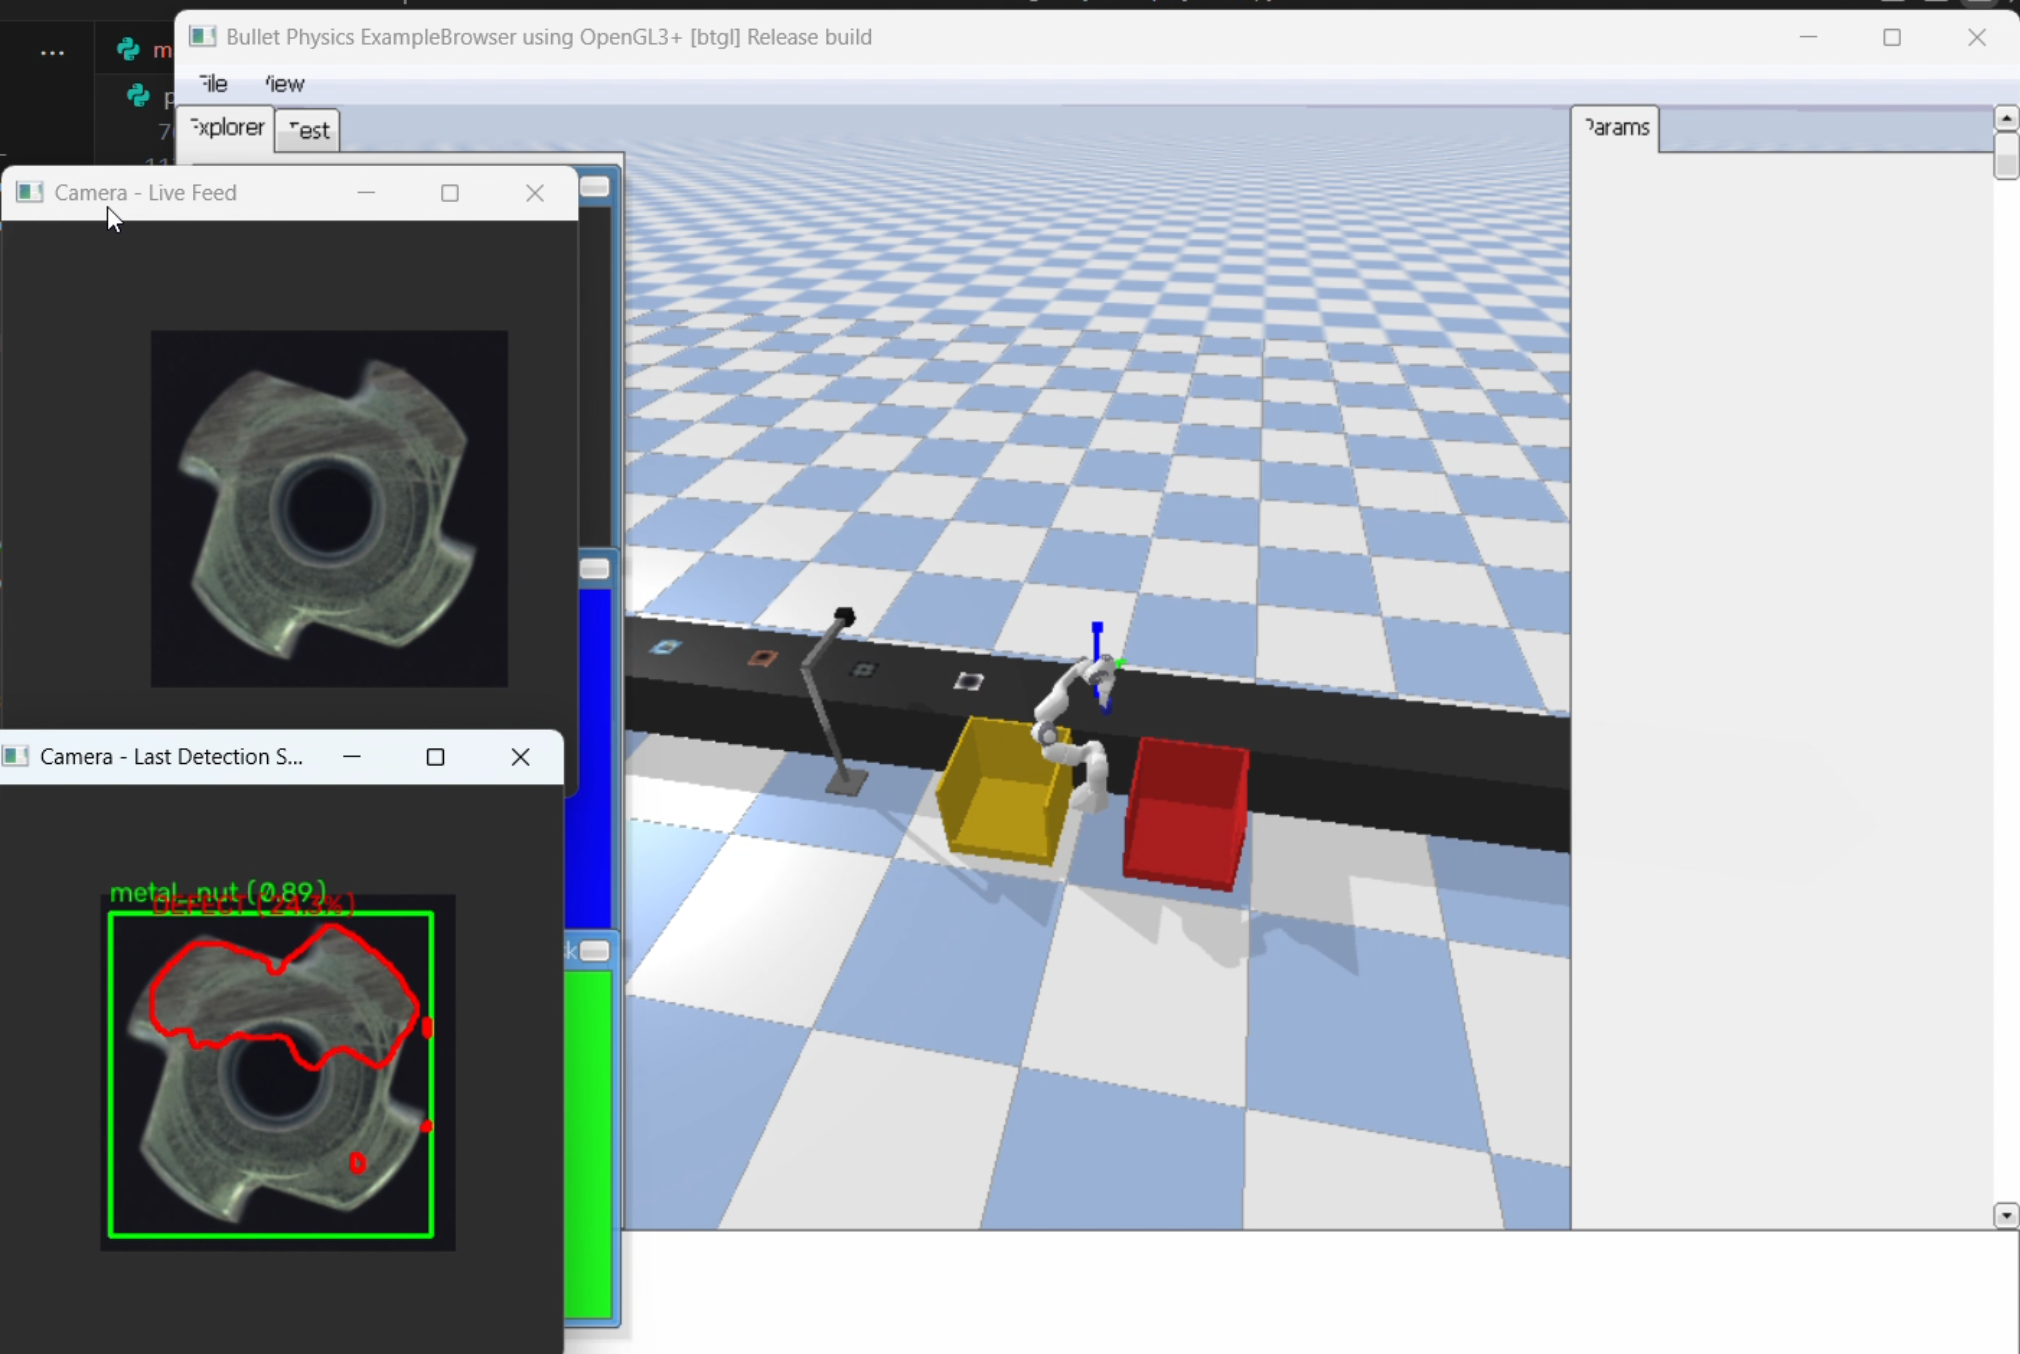
\includegraphics[width=0.85\textwidth]{img/fig31.png}
	\caption{خروجی بصری شبیه‌سازی}
	\label{fig:fig31}
\end{figure}

\begin{figure}[H]
	\centering
	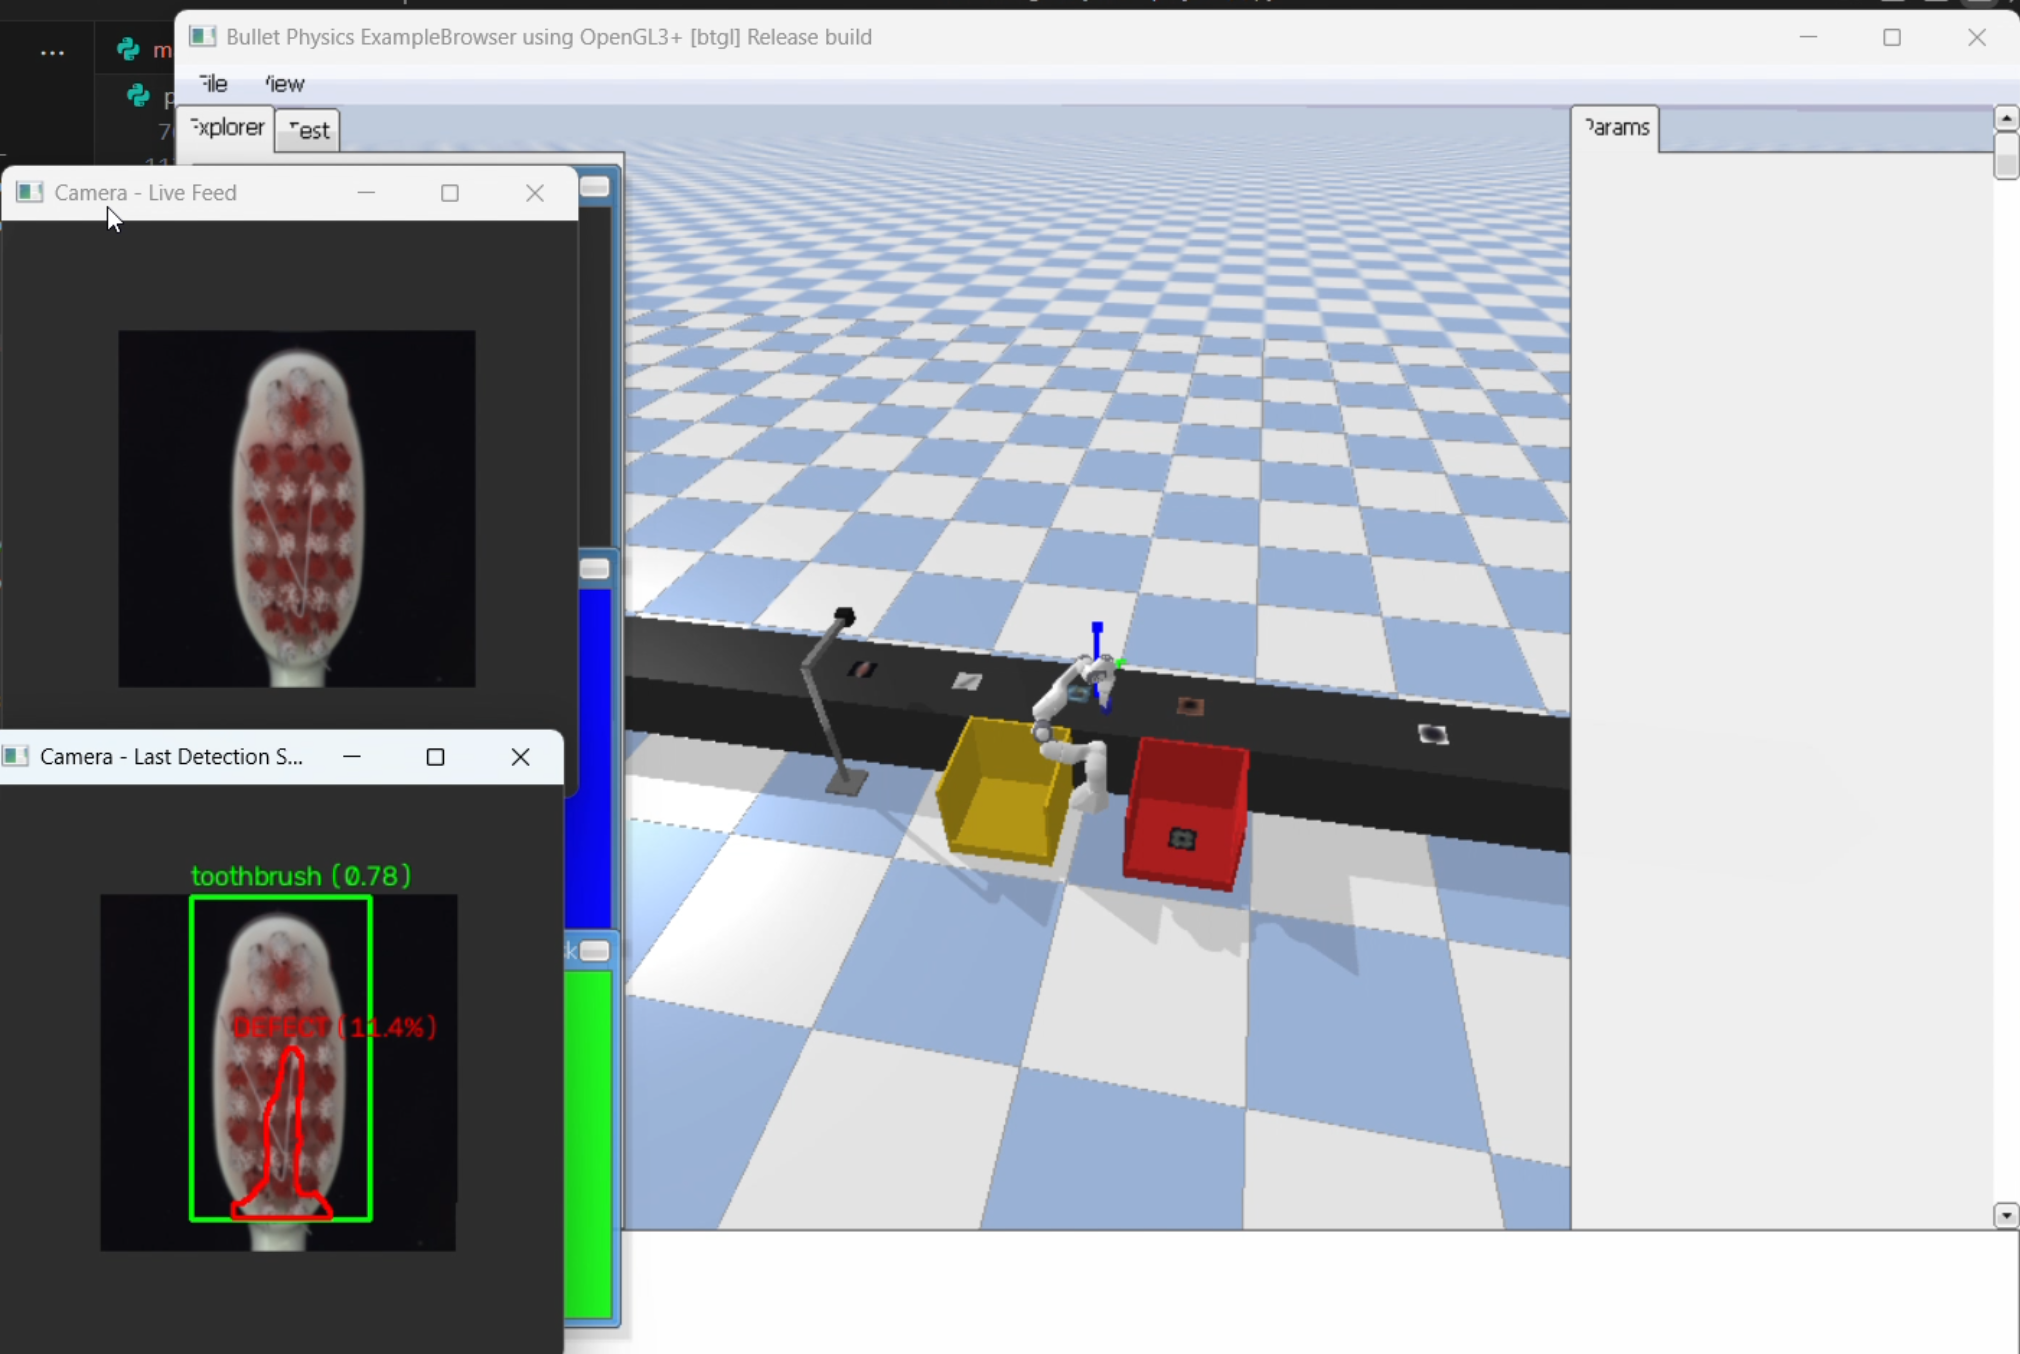
\includegraphics[width=0.85\textwidth]{img/fig32.png}
	\caption{خروجی بصری شبیه‌سازی}
	\label{fig:fig32}
\end{figure}
\subsection{جمع‌بندی اجرا}
اجرای این سناریو با توقف ایمن تمامی رزوه‌ها (\lr{Threads}) و قطع موفقیت‌آمیز اتصال موتور \lr{PyBullet} (\lr{\texttt{[SimManager] Disconnected from PyBullet}}) پایان یافت. عدم بروز هرگونه خطای مسدودکننده (\lr{Crash}) یا افت فریم شدید در حضور پردازش‌های سنگین شبکه‌های عصبی عمیق، پایداری بالای معماری نرم‌افزار، مدیریت صحیح حافظه پنهان (\lr{Caching}) و موفقیت کامل این پروژه را در پیاده‌سازی یک همزاد دیجیتال هوشمند اثبات می‌کند.







\end{document}
